% -*- mode: latex; eval: (flyspell-mode 1) -*-
\documentclass[fontsize=12,a4paper]{scrreprt}
%\documentclass[11pt,a4paper]{report}

\usepackage[T1]{fontenc}

%\usepackage{cmbright}

%\usepackage{draftwatermark}
%\SetWatermarkText{draft}
%\SetWatermarkScale{2}
%\SetWatermarkColor[gray]{0.9}

%\usepackage{newcent} % thos one is good
%\usepackage{mathpazo} % inot as good as charter
%\usepackage[urw-garamond]{mathdesign} %
%\usepackage[garamond]{mathdesign} %
%\usepackage{ebgaramond} %
%\usepackage[garamond]{mathdesign} %
%\usepackage[bitstream-charter]{mathdesign}

%\usepackage{lmodern} %
\usepackage[narrow]{inconsolata}
\usepackage{gentium} % looks very good
%\usepackage{charter} % works quite good
%\usepackage[scaled=1.05,proportional,lightcondensed]{zlmtt} % proportional - is this OK?
%\usepackage{sourcecodepro} % far too wide

\usepackage{gensymb}
\usepackage{minted}
\usepackage{hyperref}
\usepackage{graphicx}
\usepackage{xcolor}
\usepackage{framed}
\usepackage{makeidx}
\usepackage{amsmath}

\usepackage{tocloft}
%\setlength\cftsectionnumwidth{4em}
\setlength{\cftsecnumwidth}{2.5em}
\setlength{\cftsubsecnumwidth}{3.5em}

\DeclareMathOperator{\round}{round}

\makeindex

\newenvironment{warning}{\begin{framed}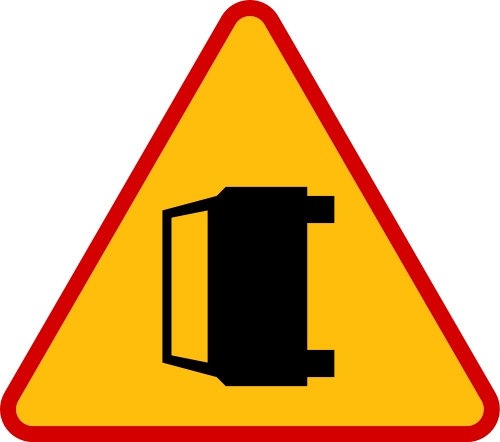
\includegraphics[width=5em]{accident-area-ahead.png}
}{\end{framed}}


\pagestyle{headings}

\usepackage{minitoc}

\begin{document}

\title{Manual for the MOONS FPU grid driver Python library
  module\\[3ex] {\LARGE (EtherCAN interface version \input{../../version})} }


\author{Johannes Nix}

\maketitle
\pagenumbering{roman}

\dominitoc



\tableofcontents

\chapter{Introduction}
\section{Related documents}

\begin{tabular}{|ll|}
  \hline
\verb+[1] VLT-TRE-MON-14620-1018+, &  FPU Verification Requirements \\
\verb+[2] VLT-TRE-MON-14620-3017+, & MOONS Fibre Positioner Verification Software Design \\
\verb+[3] VLT-TRE-MON-14620-3016+, & Fibre Positioner Communication Protocol\\
\verb+[4] FPUMovementSafetySpecification+ & Specification of safety levels for FPU movements\\
\verb+[5] VLT-ICD-MON-14620-4303+ & RFE to Instrument Software Interface Control Document \\
\hline
\end{tabular}


\section{Purpose of this document}
This document describes the Python programming interface for the MOONS
Fibre Positioner Unit EtherCAN interface module, protocol version 2.

The EtherCAN interface allows to control and move Fibre Positioner
Units (FPUs) in the MOONS FPU grid by a software interface. This
programming interface is implemented in C++. It is designed to be used
in several different contexts: Primarily, for simultaneously
controlling more than 1000 FPUs in the final MOONS astronomic
instrument. Important secondary uses are verifying and calibrating the
components of the positioning system, developing and testing of
algorithms for complex higher layers of the instrument control system,
and engineering and development of related systems and verification
software such as image analysis. For this secondary uses, a Python
module is available, which derives the lion's share of its
functionality by the C++ EtherCAN interface, while adding a small
amount of functionality which is only required for testing, or still
experimental.

Using the final verification software will not require the users to
know how to program Python.  However, several parts of the
verification software system and the MOONS instrument control software
(ICS) are initially developed and tested in Python.  The Python
interface module documented here has the function to make the
functionality of the C++ EtherCAN interface accessible from Python. As
such, the goal of this document is to describe a toolbox which can be
used to manipulate and test the FPUs as easily as possible, while the
verification software is being developed. The underlying hardware
protocol will only be exposed as much as necessary to understand the
possible states of the hardware.

NOTE: Due to tex issues, this document cannot easily be kept up to date.
(Attempting to add a new section causes tex to fail to build the manual.)
New functions and methods added recently may not be described here, or
may be mentioned in the text but not assigned a section of their own.

\section{Required knowledge}
\index{Python!introduction}
\index{Python!further information}

\paragraph{What will be helpful to know before}
It is assumed that the reader has basic knowledge of Python, or,
alternatively, a similar object-oriented language, like Java or C\#.
In the case that using Python scripts is new to the reader, it is
probably helpful to consult the tutorial for Python 2.7 at
\url{https://docs.python.org/2.7/tutorial/}.  Both the current version
of the EtherCAN interface as well as this document use Python 2.7. Python 2, which
is reaching its end of life in 2020, has some differences to Python
3. However this description will proceed in a way that differences to
Python 3 are minimised.

\index{git!further information} \index{git!getting or updating a
  repository} Also, in order to retrieve the current version of the
library, the user needs to have a minimum knowledge of either
subversion or the git version control system. This is explained, for
example, in
``\href{https://git-scm.com/book/en/v2/Git-Basics-Getting-a-Git-Repository}{getting
  a git
  repository}\footnote{https://git-scm.com/book/en/v2/Git-Basics-Getting-a-Git-Repository}''.

\section{Order of presentation}
The presentation is divided in four parts, as follows:

\begin{enumerate}
\item The first part represents a tutorial aiming at explaining
  quickly how to use the software. This also introduces basic concepts
  which are essential for understanding the subsequent manual part.
  In section~\ref{sec:minimalexample}, a minimal example is
  presented. As additional required knowledge, in
  section~\ref{sec:protectionrules} the rules for using the software
  protection layer are explained. It is recommended to read all of
  these sections before starting to operate the FPUs, and make sure
  that the datum switches work before using any datum operation.

\item The second part forms a manual which provides more complete
  information on how to operate the FPUs, and how to solve
  problems. In section~\ref{sec:settingup}, it is explained how the
  EtherCAN interface module is configured. The following sections are
  based heavily on the information given in the tutorial:
  Section~\ref{sec:datumswitchcheck} describes an important procedure
  which verifies that the datum switches are working.
  Section~\ref{sec:commontasks} explains how to perform a number of
  common tasks. Section~\ref{sec:errorhandling} explains how errors
  are handled, and can be processed in
  scripts. Section~\ref{sec:logging} details how comprehensive logs of
  the commands send to each FPU can be accessed and
  interpreted. Section~\ref{sec:healthlog} explains how the FPU health
  and performance counters are accessed, and what they mean.
  Section~\ref{sec:recovery} explains how collisions and limit switch
  breaches are handled. The final section of that part,
  section~\ref{sec:multifpu}, explains how multiple FPUs can be
  handled, especially in complex recovery scenarios.

\item The third part is the reference part, section~\ref{sec:reference}.
It lists all available commands with a comprehensive list of all their
options, and also documents the hierarchy of exceptions.
Additionally, section~\ref{sec:changelog} contains a detailed reverse
chronological list of changes to commands.

\item Finally, there is an Appendix part. It lists additional examples
  (section~\ref{sec:moreexamples}), gives a full list of software
  dependencies and how to install the software from scratch
  (section~\ref{sec:installationfromscratch}), and explains how to run
  the test gateway (section~\ref{sec:runningthegateway}).
\end{enumerate}



\section{Compatibility}
The driver software described in this manual uses the CAN protocol 2,
and requires a matching firmware version for protocol 2 in order to
work. Firmware versions for protocol 1 and 2 cannot be mixed, and an
FPU with firmware version 1 will not respond correctly to a version 2
driver.

A conceptually large internal change is that the state of the FPU is
now tracked by the FPU firmware, not more by the driver software. This
has the visible effect that even when the driver program was
terminated, it is not necessary to initialise FPUs again if they were
not powered down.

For the Python interface however, there are very little visible
changes:
\begin{itemize}
\item The \texttt{getPositions()} command has been completely replaced
  by the \texttt{pingFPUs()} command.
\item The \texttt{getCounterDeviations()} command is obsolete, because
  after a \texttt{findDatum()} operation, the residual error is
  reported automatically and stored in the FPU state.
\item Recovery of alpha limit breaches is substantially easier (and
  should also, due to changes to the movement ranges, be much safer).
\item All movement operations transmit the last direction of
    movement, and store it in the FPU state struct.
  \item FPUs with aborted movements can be recovered by using
    the new \texttt{enableMove} command.
  \item There is a new \texttt{checkIntegrity()} command which returns
    a checksum of the FPU firmware.
  \item FPUs can now be locked and unlocked, which is needed in
    instrument operation.
  \item The serial numbers and firmware versions do not need to be
    retrieved repeatedly, they are also stored in the FPU state data.

  \item A further small visible change is that error codes of CAN
    commands have different symbol names. Because this part of the API
    is now more or less stable, these symbols may be accessed via the
    \texttt{last\_status} flag, and used in test scripts. The driver
    error codes and the exception hierarchy which were already exposed
    in version 1 are unchanged.

\end{itemize}

\pagenumbering{arabic}
\part{Tutorial}

\textbf{Note:} This tutorial part assumes that the driver software is
already installed and configured to run. When this is not the case,
section~\ref{sec:settingup} on page~\pageref{sec:settingup} explains
how to do this.


\chapter{A minimal example}
\label{sec:minimalexample}
\index{example script}\index{movements!example}
\index{connect()!example} \index{EtherCAN
  interface!initialisation!example} \index{getGridState()!example}
\index{gen\_wf()!example} \index{configMotion()!example}
\index{executeMotion()!example} \index{findDatum()!example}
\index{version information!retrieving EtherCAN interface and CAN
  protocol version!example}

\minitoc


The following listing shows a minimal example of the EtherCAN
interface usage, and explains the underlying concepts step by step.

Importantly, the example assumes that the FPUs have been powered on
before, and the datum switches have been verified to work
reliably. Section~\ref{sec:datumswitchcheck} on
page~\pageref{sec:datumswitchcheck} explains how the proper operation
of the datum switches can be verified. This check should be always
done \emph{before} any \texttt{findDatum()} command is sent, because
non-working or damaged switches can lead to immediate damage of the
FPU.


\index{waveforms!example}
\index{driver!initialisation!example}
\index{getGridState()!example}
\begin{minted}[linenos]{python}

from __future__ import print_function
import FpuGridDriver
from FpuGridDriver import TEST_GATEWAY_ADRESS_LIST as gw_address
from fpu_commands import list_positions, \
       list_deviations, list_states, gen_wf
# print the driver version, just to check
print("The FPU driver version is:", FpuGridDriver.__version__,
      ", CAN PROTOCOL version:", FpuGridDriver.CAN_PROTOCOL_VERSION)

NUM_FPUS = 1 # set number of FPUs to 1
gd = FpuGridDriver.GridDriver(NUM_FPUS)
# connect to gateway with default IP 192.168.0.10
print("connecting grid:", gd.connect(address_list=gw_address))

print("getting grid state:")
grid_state = gd.getGridState()


print("issuing findDatum:")
gd.findDatum(grid_state)
print("findDatum finished")

# We use grid_state to display the starting position
print("the starting position (in degrees) is:",
       gd.countedAngles(grid_state))

# Generate a waveform which moves the alpha arm by +45
# degree, and the beta arm by +15 degree.

alpha_move = 45
beta_move = 15

# Generate the required waveform for one FPU
waveform = gen_wf(alpha_move, beta_move)

# upload the waveform to the FPU
gd.configMotion(waveform, grid_state)

# start the movement
print("starting movement by (45,15) degree")
gd.executeMotion(grid_state)

print("the reached position (in degrees) is:",
       gd.countedAngles(grid_state))

print("ready")

\end{minted}


\section{Import statements}
\index{import statements}

The import statements in lines 1 -- 4 load the following modules and
configurations:

\begin{itemize}
\item In line 1, the print function and the division operator is
  configured to work as in Python 3.

\item ``\texttt{import FpuGridDriver}'' in line 2 loads the driver
  library module. (If this import command fails, check that both
  \verb+LD_LIBRARY_PATH+ and \verb+PYTHONPATH+ have the right values.)

  \index{gateway!configuration}
  \index{IP address!of EtherCAN gateway}
\item The line ``\texttt{from FpuGridDriver import
  TEST\_GATEWAY\_ADRESS\_LIST}'' loads a default address which refers to
  the EtherCAN gateway which is used. This address would be different
  when one wants to select a different gateway. The default
  address used by the EtherCAN gateway card is 192.168.0.10,
  and the card must be connected to a private (internal) network.

\item The line ``\texttt{from fpu\_commands import \ldots}'' imports a
  few utility commands which help to display positions and to generate
  movement waveforms.


\end{itemize}

\section{Grid driver object}
\index{EtherCAN interface!instantiation}

In line 10 of the example script, the used number of FPUs is set to
one, and in line 11, the FPU grid EtherCAN interface is initialised with that
value. The returned object, which is here referenced by the Python variable
``\texttt{gd}'', is always required to access the FPUs.

\section{Driver methods}
\index{networking!see{also connect()}}
\index{connect()}
\index{EtherCAN interface!how to call methods}
The driver object allows to invoke method calls (methods are also
often called member functions) which control the FPU hardware. The
method names always start with a dot after the name of the driver
object.  So, \texttt{gd.abc()} would call method ``abc'' of the driver
object. Like normal function calls, they usually have parameters.

In this case, the method \texttt{connect()} connects the EtherCAN interface to one
or more EtherCAN gateways and starts listening to messages from the
FPUs. The parameter \texttt{gw\_address} defines to \emph{which}
gateways the EtherCAN interface listens to. Section~\ref{sec:connect}
on~\pageref{sec:connect} explains the default parameters which are
used.

As can be seen in the example, the methods have return values.  In
case of serious errors, the methods raise a Python exception.

The Python program does not need to explicitly disconnect and
de-initialise the EtherCAN interface, this happens automatically when the program
terminates\footnote{However if required, you can use the statements
  \texttt{gd.disconnect()} and \texttt{del gd}, which disconnects and
  deletes the driver object.}.



\section{Grid state variable}
\index{grid\_state variable!introduction} Almost all commands to the EtherCAN interface
receive and return a snapshot of the current state of the used FPU
(or, if there are several, of all FPUs). That snapshot is passed in a
variable called \texttt{grid\_state}. This variable contains all the
information a user might need about the state of the FPUs - their
current positions, which commands they will accept right now, whether
there are any collisions, whether the step counters have been zeroed,
whether a limit switch was hit, and so on. With each invocation of a
method, the old grid state is passed as a reference parameter, and its
new value is returned in the same variable.

To retrieve the current grid state information, the method
``getGridState()'' is used, as is done in line 16. In our listing, the
grid state data is assigned to the variable named
\texttt{grid\_state}.  The \texttt{getGridState()} function always
returns immediately, as it just takes a snapshot of the state
data. Because \texttt{grid\_state} is used so frequently, a short-hand
alternative name which many of the example scripts use is the name
\texttt{gs}.  Using the name ``gs'' is a mere convention: Technically,
these names are simply Python variable names, which can be arbitrarily
chosen by the author of a script.

\section{Moving the FPU around}
\index{movements!example}
\index{movements!overview}
The example script then proceeds to use three methods to move
the FPUs:

\begin{description}
\item[\texttt{findDatum()}] in line 20 moves the FPU to the datum
  position. After this, the internal step counters are set to zero,
  both for the alpha and for the beta arm.

  If a datum search is not possible because the arm positions do not
  allow to do that safely, a \texttt{DE\_PROTECTION\_ERROR} exception
  is returned.

  \index{waveforms!configuring}
\item[\texttt{configMotion()}] is a method which sends a table with
  movement instructions, also called ``waveform table'', to the
  FPU. In the listing, this is done in line 37. The waveform table is
  stored in the variable \texttt{waveform}, which is defined in line
  34.

\item[\texttt{executeMotion()}] in line 41 is the command which starts
  the movement of the FPU. This command returns when the movement is
  complete and the FPUs have stopped to move. In case of an error, the
  command generates a Python exception.

\end{description}

\section{Utility functions}
\index{list\_angles()|see{countedAngles()}}
\index{countedAngles()!example}
\index{list\_positions()!example}
\index{gen\_wf()!example}
The example also shows two  functions for generating movement
data, and displaying information about the FPU state:

\begin{description}
\item[\texttt{countedAngles()}] is a method which takes a
  \texttt{grid\_state} variable, refreshes its content, and displays
  the current positions of the FPUs as alpha and beta angles, in
  degree units. In these coordinates, the datum positions serve as a
  point of reference. Their value are normally -180 degree for the
  alpha datum position, and 0 degree for the beta datum positions.

\item[\texttt{gen\_wf()}] is a function which takes an (alpha,beta)
  pair of angle values, scaled in degrees, and generates a valid
  waveform which can be send to the FPU.  The waveform which is passed
  is a regular Python data structure and can be displayed and
  manipulated like any other Python object.  The user only needs to
  take care that it contains valid movement data when it is passed to
  the \texttt{configMotion()} method!

  The generated waveforms do not match the input angles exactly, as
  they are necessarily subject to rounding, which is explained below
  in further detail.

\end{description}


\section{Interactive inspection of the FPU state}
\label{sec:fpu_states_interactive_inspection}
%
\index{fpu\_state!interactive inspection}
\index{fpu\_state|see{~\emph{also} FPU state}}
\index{Python!running interactively}
\index{EtherCAN interface!configuration!example}
\index{collisions!indicator flags}
\index{grid state!interactive inspection}
\index{FPU!detailed state information}
\index{FPU!state!inspecting details}
\index{FPU!state!of grid|see{\emph{also} grid state}}
\index{state|see{FPU state}}
\index{position information!details}
\index{position information!retrieval}
\index{grid state!position|see{position information}}
\index{grid state!datum flags}
\index{datum search!flag inspection}

The grid state variable holds a large amount of detail information
about the current state of FPUs. This is by design, because upper
layers of the software need to be able to deal with complex scenarios
such as collisions, or even a pile-up of many collided FPUs, and
correct them. However, only a part of this information is required by
the verification system.

When trying to diagnose and understand errors, it is often helpful to
access this state information in an interactive way.  To do this, we
will make use of Python's capability to run any commands which appear
in a script equally well when entered interactively. In addition, the
Python interpreter can be started with the ``-i'' (interactive) option
which has the effect that after after all commands in a script have
been executed, or after any exception has been thrown, the interpreter
opens a command line or ``read-eval-print-loop'' in which commands can
be entered and executed in the interactive mode. Every time when a
typed-in expression or function call returns a value, the value is
printed out before the command prompt appears again.

For example, let's assume that the script on
page~\pageref{sec:minimalexample} is shortened to the first 36 lines
and stored to a file named \texttt{short\_script.py}. We then might
run the following interactive session (where the lines starting with
``\texttt{\$}'' and ``\verb+>>>+'' are interactive input, and
everything else is output):



\begin{minted}{python}
$ python -i short_script.py
initializing driver:  DE_OK
connecting grid: DE_OK
getting grid state:
issuing findDatum:
findDatum finished
the starting position (in degrees) is: [(-180.0, 0.0)]
>>> grid_state.FPU[0]
{ 'last_updated' : 662758.71746,
  'pending_command_set' : 0,
  'state' : 'FPST_READY_FORWARD',
  'last_command' : 1,
  'last_status' : 0,
  'alpha_steps' : 0,
  'beta_steps' : 0,
  'alpha_deviation' : 14,
  'beta_deviation' : -3,
  'timeout_count' : 0,
  'step_timing_errcount' : 0,
  'can_overflow_errcount' : 0,
  'direction_alpha' : 6,
  'direction_beta' : 6,
  'num_waveform_segments' : 19,
  'num_active_timeouts' : 0,
  'sequence_number' : 26,
  'ping_ok' : 1,
  'movement_complete' : 0,
  'alpha_was_referenced' : 1,
  'beta_was_referenced' : 1,
  'is_locked' : 0,
  'alpha_datum_switch_active' : 0,
  'beta_datum_switch_active' : 0,
  'at_alpha_limit' : 0,
  'beta_collision' : 0,
  'waveform_valid' : 1,
  'waveform_ready' : 1,
  'waveform_reversed' : 0,
  'register_address' : 0,
  'register_value' : 0,
  'firmware_version' : 2.0.0,
  'firmware_date' : '2018-01-01',
  'serial_number' : "MP000",
  'crc32' : 00000000,
  'checksum_ok' : 0,
  'sequence_number' : 26,  }
>>>
>>> gd.countedAngles(grid_state)
[(-180.0, 0.0)]
>>> gd.executeMotion(grid_state)
ethercanif.E_EtherCANErrCode.DE_OK
>>> gd.countedAngles(grid_state)
[(-135.00385502825844, 15.003335899819655)]
>>> grid_state.FPU[0]
{ 'last_updated' : 662997.43726,
  'pending_command_set' : 0,
  'state' : 'FPST_RESTING',
  'last_command' : 7,
  'last_status' : 0,
  'alpha_steps' : 5125,
  'beta_steps' : 1265,
  'alpha_deviation' : -15,
  'beta_deviation' : -13,
  'timeout_count' : 0,
  'step_timing_errcount' : 0,
  'can_overflow_errcount' : 0,
  'direction_alpha' : 6,
  'direction_beta' : 6,
  'num_waveform_segments' : 19,
  'num_active_timeouts' : 0,
  'sequence_number' : 29,
  'ping_ok' : 1,
  'movement_complete' : 1,
  'alpha_was_referenced' : 1,
  'beta_was_referenced' : 1,
  'is_locked' : 0,
  'alpha_datum_switch_active' : 0,
  'beta_datum_switch_active' : 0,
  'at_alpha_limit' : 0,
  'beta_collision' : 0,
  'waveform_valid' : 1,
  'waveform_ready' : 0,
  'waveform_reversed' : 0,
  'register_address' : 0,
  'register_value' : 0,
  'firmware_version' : 2.0.0,
  'firmware_date' : '2018-01-01',
  'serial_number' : "MP000",
  'crc32' : 00000000,
  'checksum_ok' : 0,
  'sequence_number' : 29,  }
>>>

\end{minted}

In this listing, entering the expression \verb+grid_state.FPU[0]+
displays the state parameters of FPU 0 (which is the only one we have
because \texttt{NUM\_FPUS} was set to 1).

\begin{sloppypar}
Just to pin-point two of the more important bits of information, the
fields ``\texttt{alpha\_steps}'' and ``\texttt{beta\_steps}'' contain
the current step counts of an FPU, and the fields
``\texttt{alpha\_datum\_switch\_active}'' and
``\texttt{beta\_datum\_switch\_active}'' contain the current position
of the datum switches. The field ``\texttt{state}'' contains the
current state of the FPU, ``\texttt{firmware\_version}'' contains the
version of the FPU firmware, and ``\texttt{serial\_number}'' the
serial number of the FPU, if it was stored in the firmware. One can
see that after issuing the \texttt{executeMotion} command, the state
of the FPU changes from \texttt{READY\_FORWARD} to
\texttt{RESTING}. Actually, the output of the \texttt{list\_angles()}
utility function mentioned before is normally (that is, if at least
one datum search was completed) just a scaled and shifted version of
the ``alpha\_steps'' and ``beta\_steps'' fields. The flags
\texttt{alpha\_was\_referenced} and \texttt{beta\_was\_referenced} are set to
\texttt{True} when the datum position was reached at least once since
the EtherCAN interface was started, and no collisions, limit switch breaches, or
abortMotion commands have happened since.
\end{sloppypar}

\subsection*{Capturing interactive output}
\index{capturing output} \index{troubleshooting!capturing output} To
investigate and communicate any difficulties or errors, it is
sometimes helpful to capture the interactive output. A helpful tool
for this is the Linux ``\texttt{script}'' command, which does exactly
this, and is installed on the MOONS workstation.  For further
information, please consult the ``script'' man page.



\section{FPU states}
\label{sec:fpu_states}
\index{state|see{FPU!FSM states}}%
\index{Finite State Machine|see{FPU!FSM states}}%
\index{FPU!states, how to query}%
\index{FPU!FSM states!overview}%
\index{FPU!FSM states!table}%
\index{FPU!FSM states|see{~\emph{also} fpu\_state}}%
%
The state of an
FPU is summarised in a enumeration value, which is stored in the
attribute ``\texttt{state}''. For example, the state of FPU 0 can be
retrieved by

\begin{minted}{python}

>>> grid_state.FPU[0].state
\end{minted}


\begin{table}
    \begin{minipage}{0.8\textwidth}
  \begin{centering}
\begin{tabular}{|l|p{0.7\textwidth}|}
  \hline
  \textbf{State name} & \textbf{Description} \\
  \hline
UNKNOWN & The state of the FPU is not known, the EtherCAN interface needs to
be connected to the EtherCAN gateway first and retrieve the state.\\
\hline
UNINITIALIZED & The FPU has been pinged successfully, but it was
  so far not zeroed to the datum position, so no movements are
  possible.\\
\hline
LOCKED & The FPU was locked, which inhibits movement of this
  FPU.\footnote{This is a facility provided by protocol version 2}\\
\hline
DATUM\_SEARCH & The FPU is currently searching for the datum
position.\\
\hline
AT\_DATUM      & The FPU has reached the datum position.\\
\hline
LOADING & The FPU is currently configuring a new movement waveform.\\
\hline
READY\_FORWARD & The FPU has successfully been configured with a waveform
and is ready to move in the forward
  direction of the waveform table.\\
\hline
READY\_REVERSE& The FPU is ready to move in reverse direction along the
  waveform table.\\
\hline
MOVING        & The FPU is currently moving.\\
\hline
RESTING       & The FPU has finished its movement.\\
\hline
ABORTED & The movement was aborted, either by an internal error
  in the FPU controller, or by an explicit abortMotion command.\\
\hline
OBSTACLE\_ERROR& The FPU has either detected a collision of the
  beta arm, or the alpha arm has hit the limit switch. In both cases, the
  movement was aborted. \\
\hline
\end{tabular}
\end{centering}
\end{minipage}
\caption{List of FPU states and their definitions}
\label{tab:fpustates}
\end{table}

\begin{figure}
\index{FPU!states!allowed transitions}
  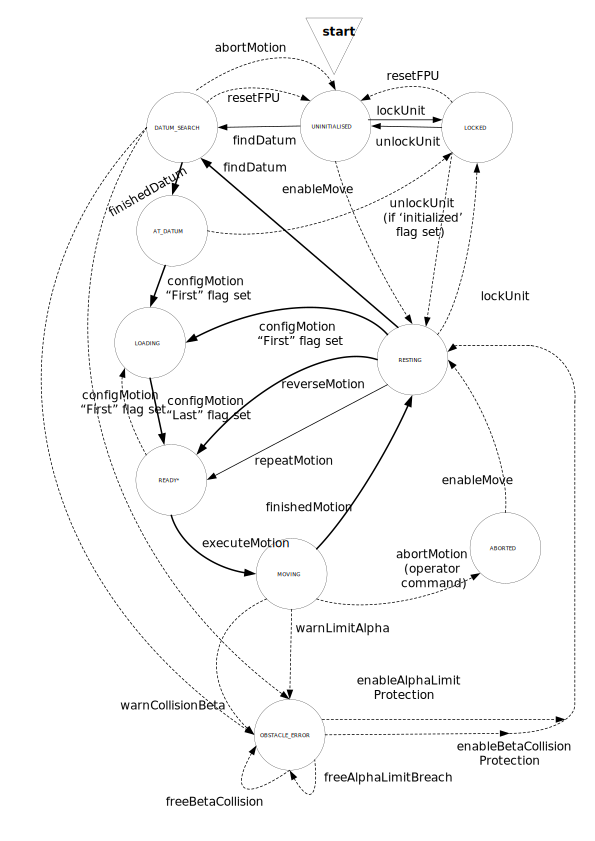
\includegraphics[width=1\textwidth]{FPU-state2.pdf}
  \caption{Allowed state transitions of a single FPU for CAN protocol
    version 2, and the associated EtherCAN interface commands and CAN messages.}
  \label{fig:states}
\end{figure}


Generally, each FPU is always in exactly one of 12 different states.
Changes can be described by the concept of a ``finite state machine'':
Each state allows a number of different commands, and commands can
change the FPU state from the current state into another allowed
state.  Some of the states are visited during any normal operation of
the FPU, and some are reached as a result of errors.
Table~\ref{tab:fpustates} on page~\pageref{tab:fpustates} lists the
different states.


\index{FPU!possible state transitions}
Figure~\ref{fig:states} on page~\pageref{fig:states} shows, as a
reference, the states of the FPU, and the possible state transitions
and commands which are allowed in protocol version 2.


\chapter{Rules to maintain integrity of the software protection}
\label{sec:protectionrules}
\index{software protection!limitations}
\index{software protection!usage rules}

\minitoc

The software protection makes it easier to ensure that the FPUs are
not damaged by out-of-bounds movements or operations that are not
supported by the firmware.

\section{Rules to observe}
The protection relies on a few conditions that must be strictly
observed at all times to keep the tracked positions valid. These
conditions are as follows:

\begin{itemize}
  \item Never use the same serial number for more than one FPU.
  \item Never move FPUs circumventing the EtherCAN interface. If FPUs are moved
    outside of the EtherCAN interface, their positions need to be stored in the
    database again, using the \texttt{fpu-admin} tool. If any driver
    instance is controlling such an FPU, before correcting the stored
    positions: exit the driver, and only after correcting re-start the
    driver.

  \item Do not use any obsolete versions of the EtherCAN interface.

  \item Never power-cycle (turn off and on again) an FPU while the
    EtherCAN interface is connected. If an FPU needs to be re-started, exit the
    program which uses the driver, restart the FPU, and start up the
    program again.  Alternatively, one can use the
    \texttt{resetFPUs()} command of the EtherCAN interface. This ensures that the
    EtherCAN interface correctly interprets the changed step count which is caused
    by the firmware reset.
  \item When first using an FPU which was newly connected to a
    gateway, always use the \texttt{trackedAngles()} method to check
    that it shows the correct position, before moving the FPU.
  \item The protection layer cannot defend FPUs from failures of the
    datum switches. Always have checked that these switches work
    before using a \texttt{findDatum()} command. The following
    section~\ref{sec:datumswitchcheck} explains in detail how a
    provisional check can be done using EtherCAN interface commands. Checks which
    address the reliability of the hardware are out of the scope of
    this document - please refer to the FPU hardware documentation.
\end{itemize}

\begin{warning}
  \textbf{WARNING: Do not power-cycle the FPU while it is connected
    to the EtherCAN interface software.}
\end{warning}


\section{Allowed operations and covered cases}
\index{software protection!allowed operations and conditions}
If the above conditions are observed, the following operations are
allowed, and designed to include the following error conditions:

\begin{itemize}
\item Moving an FPU using \texttt{findDatum()} or \texttt{executeMotion()}.
\item Reversing movements.
\item Movements which change direction multiple times.
\item Resetting FPUs, using the resetFPUs command.
\item Cancelling movements using \verb+<Ctrl>-<c>+ or \texttt{abortMotion()}.
\item Exiting and re-starting the driver program.
\item Power-cycling FPUs while the driver program is not running.
\item Controlling multiple FPU grids by different EtherCAN interface instances.
\item Trying to configure invalid waveforms.
\item Running into limit switch breaches and collisions of the arms.
\item Resuming protected operations after temporarily disabling the
  protection flag.
\item Recovering from beta collisions, using the
  \texttt{freeBetaCollision()} command.
\item Temporary or permanent loss of connectivity on the CAN bus.
\item Loss of the Ethernet connection to the EtherCAN gateways.
\item Recovery of alpha arm limit switch breaches.
\item Disconnecting an FPU from one EtherCAN gateway, and connecting
  it to another gateway connected to the same host workstation.
\item Hard power-off or loss of power of the workstation which hosts
  the driver program or the database (note that this can disrupt other
  software which is not designed for that)\footnote{The hosting
    workstation needs to use a journaling file system, such as ext4 or
    ZFS, and should not use disk encryption.}.
\end{itemize}

\section{Handling ambiguous positions}
\index{software protection!handling ambiguous positions}
\index{ambiguous positions|see{software protection}}
\index{ambiguous positions}
\index{ProtectionError!due to ambiguous  position}
%
When movements are interrupted, due to errors like collisions, or due
to \texttt{abortMotion} messages, it is possible that positions become
ambiguous. Normally, ambiguous positions are resolved by issuing a
\texttt{findDatum()} command.  It can however happen that such an
ambiguous position prevents the software protection from allowing a
new movement.  For example, if the beta arm is only known to be in a
range between -10.0\degree\ and +10.0\degree\ degrees, the software
protection cannot decide whether it should be moved clock-wise or
anti-clockwise. In this case, an error is thrown.

There are three ways to handle such a situation:

\begin{enumerate}
\item The easiest approach is to move the FPU so that its range of
  possible location does not prevent the \texttt{findDatum()} command
  any more to move in a unambiguous direction. For example, if in the
  case given above, the FPU is moved by 15\degree\ degrees
  anti-clockwise, its new position will still be ambiguous, but it
  will be in the range from +5.0\degree\ to
  +25.0\degree\ degrees. (When the FPU is not in initialized state, it
  will be necessary to pass the keyword parameter
  \texttt{allow\_uninitialized=True} to the corresponding
  \texttt{configMotion()} command, and also to issue an
  \texttt{enableMove() command}. However, it is not at all necessary
  to disable the software protection.)

  Now, the findDatum command will simply perform an clock-wise datum
  search, without needing any further information.

\item Alternatively, in a few cases, it can be necessary to exit the
  driver, measure the position, and assign a new position to the FPU,
  using the \texttt{fpu-admin init} command.

  \index{software protection!disabling}
  \index{hardware protection!testing}
\item In theory, it is also possible to disable the software
  protection.  This is almost never a good idea. Disabling the
  software protection should only be done when it is necessary to move
  the FPU outside of its safe range of positions. This is only needed
  when explicitly testing hardware protection functions.
\end{enumerate}

The next section explains how to test the proper functioning of the
datum switch hardware in a safe way.


\part{Manual}

\chapter{Setting up the library module}
\label{sec:settingup}
\index{driver|see{also: EtherCAN interface}}
\index{EtherCAN interface!building}

\minitoc


This section deals with retrieving, installing and configuring the
EtherCAN interface module. On the MOONS workstation at UKATC, it can
be skipped because the FPU EtherCAN interface is already installed.
In this case, you can proceed directly with
section~\ref{sec:minimalexample} on page~\pageref{sec:minimalexample}.

\section{Installing required dependencies for a new installation}
For a new installation, a number of required dependencies should be
installed on a 64-bit Linux system. The detailed list of dependencies,
and how to install them is explained in
Appendix~\ref{sec:installationfromscratch} on
page~\pageref{sec:installationfromscratch}.


\section{Getting the source code}

To set up the library module, it is first necessary to retrieve a
current copy of its source code.

\subsection{Using a packed archive}
Without direct access, this can be done by unpacking a tar archive
with the latest sources.


\subsection{Using network access}
On the moons-pc01 workstation, this can be done using the command
\mint{bash}|git clone /home/jnix/fpu_driver| This creates a new
directory with the name \texttt{fpu\_driver} and populates it with the
source code.

Alternatively, a fresh copy can be retrieved from the UKATC dalriada
server. Doing this this requires a personal user account on that
server. Assuming the account name is \texttt{carl}, this is done by
the command
\index{git!repository setup}

\mint{bash}|git clone carl@dalriada/sw/sw4/jnix/MOONS/fpu_EtherCAN interface|

After entering the password for user \texttt{carl}, the
source code is copied into the new folder \texttt{fpu\_driver}.

\paragraph{Refreshing the source code from git}
\index{EtherCAN interface!building!update or change version}
To refresh the source code, change the
working directory to \texttt{fpu\_driver},
and issue the command

\mint{bash}|git pull|

\subsection{Using the ESO subversion repository}

This repository contains the current development version of the module
for hardware protocol 2. It can be retrieved using the URL
\url{http://svnhq1.hq.eso.org/p1/branches/MOONS/FibrePositioner/MOONS2/ICS/mpifps/}.

The \texttt{"make"} commands described in the following need to be run
in the top-level folder. This uses a temporary \texttt{Makefile} which
ignores the other ICS components. Running the code from this
development branch requires to run either the included EtherCAN
hardware simulation (as described in
Appendix~\ref{sec:runningthegateway}), or compatible FPU firmware for
hardware protocol v2.

\section{Building specific revisions}
\index{git!get specific version}
\index{EtherCAN interface!building!specific version}
In the default case, the library is build from
the master branch of the git repository.
The master branch contains the most current
working version.
In some cases, it might be required to
use a specific revision of the library.
Assuming that we need, as an example,
to build version 1.5.2 of the library,
checking out this revision is done with the
command

\mint{bash}|git checkout v2.1.1|

After this, one can proceed with building the library as normal. To
switch back to the master branch, issue the command\footnote{
  previously, the master branch tracked the CAN protocol version 1.
  The master branch has been changed to track the can protocol 2 branch
on September 19, 2019.}

\mint{bash}|git checkout master|


\section{Building the library module}
\index{EtherCAN interface!building}
To build the Python library module,
change the working directory to \texttt{fpu\_driver},
and issue the command \mint{bash}|make wrapper|

In order for this to work, the required dependencies need to be
installed. For the MOONS workstation at UK ATC, this is always the
case. To install these dependencies on other computers, follow the
detailed instructions in the appendix
section~\ref{sec:installationfromscratch} on
page~\pageref{sec:installationfromscratch}.  A more concise summary is
given in the text file ``\texttt{python/doc/INSTALL}''.

\section{Enabling debug output of CAN messages}

Beginning with EtherCAN interface version 0.5.3, a very comprehensive
log of sent and received CAN messages is enabled by default. For long
running tests, the logging might need to be set to a lower level of
detail in order to keep the used disk space in reasonable limits.  See
section~\ref{sec:logging} on page~\pageref{sec:logging} for the
location of these logs, and any further details.


\section{Environment configuration}
\label{sec:environmentconfiguration}
\index{EtherCAN interface!configuration}
\index{setup!environment variables}
\index{environment variables}

For the Python module to work, the directory \texttt{/user/local/lib}
(or, more general, the path to which the boost::python library is
installed to) needs to be added to the environment variable
\texttt{LD\_LIBRARY\_PATH}.

Further, the library uses a lock file to prevent that different
processes send simultaneously commands to the same gateway. To access
the lock file, all user accounts which use the driver software need to
be member of the Unix group defined in the environment variable
\texttt{MOONS\_GATEWAY\_ACCESS\_GROUP}. The default name for that
group is \texttt{"moons"}.

Also, it is probably useful to add the \texttt{python} directory
within the driver package, and also the current directory to the
environment variable \texttt{PYTHONPATH}, so that the EtherCAN
interface module can be found independently from the current working
directory.  Assuming a standard Ubuntu or Debian setup, this can be
done by adding the following lines to the file \texttt{.bashrc} in the
user-specific home directory:

\begin{minted}{bash}
  export LD_LIBRARY_PATH=$LD_LIBRARY_PATH:/usr/local/lib
  export PYTHONPATH=$PYTHONPATH:$HOME/fpu_driver/python:.
\end{minted}

To run the \texttt{fpu-admin} Python script, which manages the FPU
position database, it is also recommended to include the above
directory in the PATH environment variable, like this:

\begin{minted}{bash}
  export PATH=$PATH:$HOME/fpu_driver/python
\end{minted}


Further, it is recommended to set the default log directory to point
to a file system which is writable and has a lot of free space, for
example:
\begin{minted}{bash}
  export FPU_INTERFACE_DEFAULT_LOGDIR=/moonsdata/logfiles
\end{minted}

\index{software protection!configuration}
\index{software protection!access permissions}
%
One more setting is required: This version of the EtherCAN interface
uses a position database, which tracks positions and state of FPUs at
any point in time. Importantly, this database needs to be
\emph{global} (that is, for all users) for the workstation on which
the EtherCAN interface software is running. To configure it, the
environment variable \texttt{FPU\_DATABASE} needs to be set in the
configuration file \texttt{/etc/profile} as follows:

\index{software protection!environment variables}
\index{LMDB database!environment setup}
%
\begin{minted}{bash}
  FPU_DATABASE=/var/lib/fpudb
  export FPU_DATABASE
\end{minted}

If this variable is not set, the FPU position database will not be
used. In this case, the hardware protection capability, which is
implemented in the Python wrapper, is not available.

\index{LMDB database!access permissions}
The directory specified has to be created to be writable by any user
which runs an FPU EtherCAN interface. It is therefore necessary to set up any user
which runs the FPU EtherCAN interface to belong to the same user group, and make
the directory writable by any member of this group, using the Unix
``chmod'' and ``chgrp'' commands.

\paragraph{Note on memory usage}
\index{virtual memory usage}
\index{troubleshooting!memory consumption}%
\index{memory leak|see{virtual memory usage}}%
%
As a side note, the FPU position database uses LMDB to enable
fail-safe storage and logging. This is a fast, thread-safe key-value
storage which uses large memory-mapped files.  LMDB can often use a
large amount of virtual memory. This is not a bug and especially not a
memory leak, as only a small fraction of this data is actually loaded
into RAM.


\section{Supported firmware versions}
This EtherCAN interface requires FPU firmware version 2.0.x to support
all regular features. Older versions of the FPU firmware are not fully
supported, and do not handle CAN message priorities correctly.  See
section~\ref{sec:firmware_compatibility} for details which
functionality is missing for older versions.

\section{Hardware configuration and addressing}
\subsection{Addressing of FPUs}
\label{sec:hardwareaddressing}
\index{addressing!FPUs}
\index{indexing FPUs}
\index{FPU IDs!configuration}
\index{CAN ID}
\index{FPU!addressing}
\index{FPU!hardware configuration}
\index{networking!FPU addressing}
Messages to an individual FPU are sent using a logical number, the FPU
ID, which starts at 0 and goes up to a maximum value. Gaps in the
sequence of used logical numbers are not supported.

The messages from the EtherCAN interface to FPUs are transported by two layers of
hardware.

\index{EtherCAN gateway!configuration} \index{IP address!of EtherCAN
  connection} \index{port number!of EtherCAN connection} First, the
messages are transmitted by an Ethernet socket connection to up to
three EtherCAN gateways. To connect to each gateway, its IP address
and port number are used. The default IP number, to which the EtherCAN
gateway card is configured, is "\texttt{192.168.0.10}", and the
connection uses port 4700 by default. In this case, the EtherCAN
gateway (or if several are used, all of them) needs to be connected to
a private network interface to which IP packets to network
\texttt{192.168.0.0/24} are routed.

From the selected gateway, the messages are then forwarded to up to
five CAN buses. Each bus connected to a gateway is identified with a
number as well, and is connected to up to 72 (currently, 67) FPUs.
\index{DIP switch} To identify each FPU in a setup with many FPUs,
they have to use a CAN ID which is unique on each bus, \emph{and is
  different from zero}. This ID is physically configured by manually
toggling a DIP switch in the FPU's electronics board. The current
EtherCAN interface uses a fixed continuous mapping (basically, array
indexing) from the translation of FPU IDs to gateway number, bus
number, and CAN ID\footnote{Future versions of the software will relax
  this restriction}.

This results in that each FPU has a physical address with three
elements: gateway number, bus number, and CAN ID.

\emph{For addressing a single FPU, this simply means that its CAN ID
  needs to be set to one, which means its DIP switch needs to be set
  to the delivered configuration. That FPU then needs to be connected
  to the first bus on the first gateway}.

\textbf{Note:} The current hard-wired address mapping between FPU
logical numbers and the (gateway number, bus number, CAN ID) tuple
will be made more flexible in future versions of the EtherCAN
interface. The current mapping will remain the default value.


\subsection{Configuring gateways to start and stop FPUs synchronously}
\label{sec:synccommand:explanation}
\index{SYNC command!explanation}
\index{SYNC command!hardware set-up}
\index{troubleshooting!FPUs do not start or stop at the same time}
\index{troubleshooting!only FPUs from one gateway start}
\index{troubleshooting!gateways incorrectly connected}

The EtherCAN gateway hardware provides a feature to start or stop FPUs
which are attached to different buses, and to different gateways, at
exactly the same time. This is achieved by sending a SYNC message to
one gateway, which will trigger sending of a pre-configured message to
all buses.

For this to work, if using different gateways, \textbf{the gateways
  need to be connected accordingly.} If this connection were omitted,
SYNC commands would not work, and collisions would be the
consequence. The Python \texttt{fpu\_driver} wrapper supports sending
of SYNC commands for the \texttt{executeMotion()}, and the
\texttt{abortMotion()} method. For the former, a SYNC command is uses
if a specific keyword argument flag is set -- see
section~\ref{sec:synccommand} on page~\pageref{sec:synccommand} for
details. For the \texttt{abortMotion()} method, which is used to
instantaneously and safely stop movements, a SYNC command is used by
default (see section~\ref{sec:abortMotion} for more information).

\begin{warning}
  \textbf{WARNING: If you connect FPUs to several gateways to operate
    together, make sure that the EtherCAN gateways are connected
    properly to ensure transmission of SYNC commands.}
\end{warning}


\section{Configuring serial numbers and setting initial positions}
\label{sec:setinitialposition}
\index{software protection!configuration and setup}
\index{LMDB database!initialisation}

\paragraph{Initialising an FPU}

(Note: This step can be skipped if the LMDB protection feature is not
used, for example when only testing electronic components rather than
mechanical hardware. In this case, only a limited ``unprotected''
driver layer is available.)

Before any FPU can be used with the EtherCAN interface, two commands
need to be performed to configure the hardware protection feature:

\begin{enumerate}
\item The serial number of the FPU needs to be flashed to the
  NVRAM of the FPU motion controller. This allows the software
  to recognise the FPU.
\item The initial position of the alpha and beta arm needs to
  be stored in the FPU database.
\end{enumerate}

To do this, the FPU needs to be connected to the EtherCAN gateway with
a known logical ID, determined by the CAN bus ID explained
above. Also, the gateway needs to be connected to the workstation.

Let's assume that the serial number is represented by the shell
variable \texttt{serialnumber}, the logical FPU id by the variable
\texttt{fpu\_id}, the initial alpha arm position by
\texttt{alpha\_position}, and the beta arm position by
\texttt{beta\_position}. The angular positions are given in degrees,
and with the coordinate offsets used in the instrument. By default,
this means the alpha datum position is at -180\degree\ degrees, and the beta
datum position at zero degrees.

Then, the following two commands need to be issued:
%
\index{initializing serial numbers!using fpu-admin tool}%
\index{configuring serial numbers!using fpu-admin tool}%
\index{serial numbers!initial assignment using fpu-admin tool}%
\index{ProtectionError!caused by identical serial numbers, how to prevent}%
\index{troubleshooting!how to prevent ProtectionError caused by identical serial numbers}%

\begin{minted}{bash}
  fpu-admin flash ${serialnumber} ${fpu_id}
  fpu-admin init ${serialnumber}${alpha_position} ${beta_position}
\end{minted}

The first command writes the serial number to the NVRAM of the FPU
controller. This needs to be done only once (except when the
electronics PCB of that FPU is replaced by another PCB). The serial
number must never be used for another FPU. (As a protective measure,
the command checks that the serial number wasn't used before. This
check can be disabled by passing the \texttt{--reuse\_sn} flag.)

The second command stores the position of the FPU in the position
database. The position has to be qualitatively correct whether the
alpha arm is in the safe zone and whether the beta arm needs to move
into a clock-wise or anti-clockwise direction to datum. It is also
possible to specify position ranges as measurement uncertainty
intervals in the form of Python list literals, enclosed in double
quotes:
\index{software protection!handling ambiguous positions}
\index{ambiguous positions}
\begin{minted}{bash}
  fpu-admin init ${serialnumber} "[0, 1.5]" "[3, 6.5]"
\end{minted}


Importantly, storing the position has to be repeated when it should
occur that the stored position is not matching the actual
position. Apart from driver bugs, this can only happen if the FPU is
moved by something else than the FPU EtherCAN interface.

\paragraph{Viewing FPU position dates}

The database record can be viewed and verified by using the command

\begin{minted}{bash}
  fpu-admin list1 ${serialnumber}
\end{minted}

Assuming the initial positions were alpha = -179\degree\ degrees and beta =
1\degree\ degrees, this should show data similar to the following output:

\begin{minted}{python}
jnix@nippes:~/MOONS/fpu_driver/python$ ./fpu-admin list1 PT01
['./fpu-admin', 'list1', 'PT01']
('PT01', 'apos') : [[-179.0, -179.0], -180.0]
('PT01', 'bpos') : [[1.0, 1.0], 0.0]
('PT01', 'wf_reversed') : False
('PT01', 'alimits') : [[-180.0, 179.6], -180.0]
('PT01', 'blimits') : [[-179.3, 150.3], 0.0]
('PT01', 'bretries') : 3
('PT01', 'beta_retry_count_cw') : 0
('PT01', 'beta_retry_count_acw') : 0
  ....
\end{minted}

What can be seen from the above example is that both the alpha
position ('apos') and the beta position ('bpos') are stored as a
braced pair of identical numbers, followed by an additional
number. The number pair indicates the position, and the additional
number indicates the offset of the datum position, which is by default
-180\degree\ degrees for the alpha arm, and 0\degree\ degrees for the beta arm. One
could ask why the arm positions are represented as a number pair. The
reason is simple: The database is designed so that it can, if
required, represent uncertainty around the arm positions as an
position interval. In that case, the number pairs would represent
start and end of an interval of possible positions.

The intervals ``alimits'' and ``blimits'' describe the ranges which
are considered safe by the software. They can be adjusted on an
per-FPU basis if required, using \texttt{fpu-admin alimits} and
\texttt{fpu-admin blimits}.

The \texttt{fpu-admin} tool can also be used to print a list of datum
aberrations (the difference between the ideal datum position, and the
step count at which datum was actually found), and a time-series of
counters. This is described in the reference part in
section~\ref{sec:healthlog}. More commands and options are shown if the
tool is run with the command-line option ``-h'' or ``--help''.

\section{Database maintenance}
\index{LMDB database!maintenance, backup} The position database is
required to operate the FPUs in the normal (protected) operation mode,
and will also hold some data gathered during calibration of the
FPUs. It is therefore necessary to back it up regularly.  It can be
backed up by copying the content of the directory defined in the
\verb+$FPU_DATABASE+ environment variable. For this, the dedicated
backup tool for LMDB, \texttt{mdb\_copy} should to be
used. \texttt{mdb\_copy} is safe for backing up a database which is in
use at the same time.

The database can be used by several EtherCAN interface instances at once, each of
them controlling different FPUs. When the involved EtherCAN interfaces are not
running, FPUs can be switched from one gateway to another one - the
information in the database will remain valid.

\section{Software protection flag}
\label{sec:protectionintro}
\index{hardware protection!function}
\index{soft\_protection flag}
\paragraph{Protecting instrument hardware}
The FPU control chain uses a layered approach to make sure that fibre
positioner units do not get damaged.

\paragraph{Hardware protection}
At the bottom layer, there is an electronic collision protection,
which will switch off the motors and send a warning message if two
FPUs touch each other. This protection level is called ``hardware
protection''.

\index{wear and tear} \index{avoiding hardware damage}

However, even if a direct damage should be avoided by this protection,
activating it involves that the motors are suddenly stopped, which
decreases the precision and can significantly increase wear and tear,
thus reducing the life time of the stopped FPU. Therefore, the
hardware protection should be used only at an emergency
level. Furthermore, some situations are not covered by it,
specifically if the FPU arms are moved into the dead zones.

\paragraph{Software protection}
For these two reasons, the EtherCAN interface software performs
comprehensive additional checks which should ideally ensure that no
out-of-range movements occur. These checks are performed every time an
FPU is moved, or configured to move, and are named ``software
protection''.  For all normal movements of FPUs, this protection
should be left active.

\paragraph{Deactivating the software protection}
In some situations, specifically if the hardware protection or the
alpha datum switch needs to be tested, it can be necessary to switch
off and deactivate this software protection layer. This can be done
using the ``\texttt{soft\_protection}'' keyword argument when calling
the corresponding EtherCAN interface methods. Passing the value
``\texttt{soft\_protection=False}'' will switch the software
protection check off. When this is done, the entire responsibility
with operating the FPUs safely is with the user. It is highly
recommended to refer to additional documentation (especially
FPUMovementSafetySpecification.docx, the actual RFE to software ICD
document, and additional hardware and firmware documentation), to
assess which operations are safe.

It is also possible to de-activate any protection by using a special
driver class with the name \texttt{UnprotectedGridDriver}. This class
is useful for testing purposes, but should not be used with valuable
hardware.



\section{Communication protocol versions}
\index{protocol!see{\ CAN protocol}} \index{CAN protocol!versions}
\index{protocol!versions}
\index{CAN protocol versions! version 1 capabilities} The FPU EtherCAN interface
sends commands to the fibre positioner units, which use a specific
communication protocol. This protocol needs to match the FPUs firmware
and its capabilities. The current version of the EtherCAN interface (version
2.0.x) uses ``communication protocol version 2.0'', which has some
differences to earlier versions.

A significant difference in the hardware protection capabilities is
that cases in which the alpha arm of the FPU hits the limit switch can
be recovered in exactly the same way as a beta arm collision. This is
explained in section~\ref{sec:recovery} on
page~\pageref{sec:recovery}.


The functionality described in this document is supported by EtherCAN
interface versions equal or newer than 2.1.0 and an FPU firmware that
supports the CAN protocol version 2.0.x or later. Earlier firmware
versions do not work with this driver software version.

The next sections are intended as a tutorial on how to control and
operate FPUs. As usual, the operations are presented so that the most
basic concepts are introduced first, and more difficult commands and
concepts which build on that later. For this reason, it is first shown
in section~\ref{sec:minimalexample} how to perform basic movements,
before explaining in section~\ref{sec:datumswitchcheck} how the switch
operation is tested. Nevertheless, it is highly recommended to have
test the switch operation tested before doing any further operations
with the FPU.

\begin{warning}
  \textbf{WARNING: Before first issuing a \texttt{findDatum()}
    command, make positively sure that both the alpha arm datum switch
    and the beta datum switch work. Especially for the alpha arms,
    defective datum switches will likely cause the datum command to
    damage the hardware. The EtherCAN interface software cannot protect against
    this.}
\end{warning}



\chapter{Checking the datum and limit switches}
\label{sec:datumswitchcheck}
\index{limit switch!testing}
\index{datum switch!testing}
\index{hardware protection!testing}

During initial testing of each FPU, it is advisable to test the
function of the switches -- especially the alpha limit switch --
without performing a datum operation. The reason for this is that if
the alpha limit switch should not work, the datum operation would
probably damage the FPU irreparably.

The following section describes how to check that the datum and limit
switches of an FPU are working.

\section{How to retrieve the switch state}
\index{alpha limit switch!checking state}
\index{limit switch!check the state}


To test the switches, the FPU needs to be be driven manually to a
position where the corresponding switch is required to engage. At this
point, one can use the command

\begin{minted}{python}
  gd.getSwitchStates(grid_state, fpuset=[])
\end{minted}

to retrieve the state of the switches.


\section{Required information}

To begin this test, it is necessary to know the exact safe operation
ranges of the alpha and beta arm. These values depend on hardware and
FPU firmware revisions and are currently still subject to change.
They are described in document
[4],~``FPUMovementSafetySpecification.docx''.  The following
description assumes that the position after performing a datum
operation is (-180\degree, 0\degree) degrees, that both switches are off at
positions (-175\degree, 5.0\degree), and both switches on at positions (-180.2\degree,
-0.2\degree).

\section{Test procedure, explained step-by-step}
To test the datum switches, perform the following steps:

\begin{enumerate}
\item If the EtherCAN interface is connected, disconnect it first.

\item Make sure that the FPU database contains the correct alpha and
  beta arm positions for the FPU which is examined. Do this using
  the command
  \begin{minted}{bash}
    fpu-admin ${serialnumber} list1
  \end{minted}

  The result should look like that:

  \begin{minted}{python}
    ['./fpu-admin', 'list1', 'PT01']
    ('PT01', 'apos') : [[-180.0, -180.0], -180.0]
    ('PT01', 'bpos') : [[0.0, 0.0], 0]
    ('PT01', 'wf_reversed') : False
    ('PT01', 'alimits') : [[-180.0, 179.6], -180.0]
    ('PT01', 'blimits') : [[-179.3, 150.3], 0.0]
    ....
  \end{minted}

  This indicates that the alpha arm is at position -180\degree\ degrees,
  using a datum offset of -180\degree\ degrees, and the beta arm is at
  0\degree\ degrees.

  If the positions are not correct, proceed as described in
  section~\ref{sec:setinitialposition} on
  page~\pageref{sec:setinitialposition}. The further explanation
  assumes that the FPU position is at the numbers shown above.

\item Connect the EtherCAN interface and run a \texttt{pingFPUs()} command.

\item Move the FPU so that it is within the normal range, and with
  certainty not touching the datum switches.

  As a normal movement configuration requires
  that a datum search has been performed before,
  it is necessary send an \texttt{anableMove() command first}, and
  also to pass the \texttt{allow\_uninitialized=True}
  flag to the configMotion command:

  \begin{minted}{python}
    w = gen_wf(5,5)
    gd.enableMove(0, gs)
    gd.configMotion(w, gs, allow_uninitialized=True)
    gd.executeMotion(gs)
  \end{minted}

\item Verify that both switches are off:

  \begin{minted}{python}
    gd.getSwitchStates(gs)
  \end{minted}

\item Now, move the FPU so that it just activates the datum
  switches. The movement interval needed depends on firmware version
  and offsets used.  In addition to the options used in the first
  movement, it is now necessary to disable the protection layer by
  passing the ``\texttt{soft\_protection=False}'' keyword argument.
  With firmware version 1.3 and an initial position of (-180, 0), this
  will be reached by using the command

    \begin{minted}{python}
      w = gen_wf(-5.2,-5.2)
      gd.enableMove(0, gs)
      gd.configMotion(w, gs, allow_uninitialized=True,
                      soft_protection=False)
      gd.executeMotion(gs)
    \end{minted}

    The FPU should now be at an absolute position of (-180.2, -0.2), and
    touching both switches.

  \item Now, verify that both switches are on:
    \begin{minted}{python}
      gd.getSwitchStates(gs)
    \end{minted}

    Finally, the FPU arms can be moved back into the safe zone, using
    the command
    \begin{minted}{python}
      gd.enableMove(0, gs)
      w = gen_wf(5.2,5.2)
      gd.configMotion(w, gs, allow_uninitialized=True,
                      soft_protection=False)
      gd.executeMotion(gs)
    \end{minted}

\end{enumerate}

If this test does not have the expected result, the cause is likely to
be a hardware failure, which makes the FPU unusable until it is
resolved.

\chapter{Common tasks}
\label{sec:commontasks}

\minitoc

The following sections describe several common tasks
and describes which commands can be used to perform them.


\section{Checking the connection}
\index{networking!check}
\index{networking!example}
\index{errors!connection}
\index{connection,checking the}
\index{troubleshooting!connection problems}
\begin{samepage}
At some points, it is of interest what the state of
the connection to the CAN gateway and of the FPUs is.
This can be achieved by the following commands:
\begin{minted}{python}
grid_state = gd.getGridState()
grid_state.interface_state
\end{minted}
The return value is the connection state of the EtherCAN interface, which is
\texttt{DS\_CONNECTED} if the connection is live.  In the case that the
connection fails, it is still possible to retrieve state information
on the FPUs, but it cannot be refreshed any more until the connection
is re-established using the \texttt{connect()} method of the driver
object.
\end{samepage}

\index{connection errors!example} Of course, it is possible that the
connection between EtherCAN interface and EtherCAN gateway works, but that an FPU
does not respond, for example, if the CAN bus connection wiring is
broken, or the FPU has no power. This can be checked by the commands:

\begin{minted}{python}
  gd.pingFPUs(grid_state)
  grid_state.FPU[0].ping_ok
\end{minted}

In the case that the FPU responds, the returned value is
\texttt{True}.  If the FPU does not respond, the value of the
\verb+ping_ok+ becomes \texttt{False}.

Errors both during making the socket connection, and when sending
commands to the FPUs cause a \texttt{ConnectionFailure} exception to
be thrown, like in this log file:

\index{exceptions!example}
\begin{minted}{python}
  $ python -i test_mockup/test_asyncMotion.py
connect: Connection refused
Traceback (most recent call last):
  File "test_mockup/test_asyncMotion.py", line 12, in <module>
    print("connecting grid:", gd.connect())
  File "/sw/sw4/jnix/MOONS/fpu_driver/python/FpuGridDriver.py", line 65, in connect
    return self._gd.connect(address_list)
    fpu_driver.ConnectionFailure: DE_NO_CONNECTION: The FPU Driver
    is not connected to a gateway.
>>>
\end{minted}


The associated error message and enumeration symbol should be
sufficient to determine the cause of the problem. A comprehensive list
of exceptions and error codes is given in section~\ref{sec:errors} on
page~\pageref{sec:errors}.

\paragraph{Recovery form connection errors}
If the connection to a gateway is lost, the \texttt{connect()} method
of the EtherCAN interface needs to be called again to re-establish it.

\index{troubleshooting!connection errors}%
\index{troubleshooting!CAN time-outs}%
%
If a specific FPU does not respond, each command to it will result in
a time-out, until it responds again. Other FPUs will be unaffected.
Failures to respond can be caused by cabling problems, a missing
termination resistance on the CAN bus, or an invalid CAN id
configuration (which is explained in
section~\ref{sec:hardwareaddressing} on
page~\pageref{sec:hardwareaddressing}). Another very likely cause of
command time-out errors are hardware failures which prevent FPU
operations from completing. In this case, the involved FPUs are
probably broken.


\section{Checking the FPU firmware, its integrity, and the FPU serial numbers}

After having a working connection, it is useful to check for the
correct firmware version, the firmware integrity, and the serial
number of the addressed FPUs.

\subsection{Checking the protocol version}
\index{checking for a correct protocol version}%
%
The value \texttt{FpuGridDriver.CAN\_PROTOCOL\_VERSION}
returns the major version number of the CAN protocol
which the driver implements. Because a script might
not work as expected, it can be useful to check it
automatically in the top level python script like that:

\begin{minted}{python}
  assert(FpuGridDriver.CAN_PROTOCOL_VERSION == 2)
\end{minted}


\subsection{Checking the firmware version}
\index{check firmware version of FPU}%
\index{troubleshooting!checking firmware version}%
Next, the version of the firmware running on the FPUs can be checked
with the command

\begin{minted}{python}
  gd.printFirmwareVersion(grid_state)
\end{minted}

It returns a list of FPUs with the corresponding version of the
version and data of the firmware in the FPU's motion controller.

It is possible that some tests rely on a certain minimum
firmware version being present on the controllers.
This can be checked with the method

\begin{minted}{python}
  gd.minFirmwareVersion() >= (2, 0, 3)
\end{minted}


\subsection{Checking the firmware integrity}

As best practice, any important tests should also check beforehand
the integrity of the flashed firmware. This can be done with
the following command:

\begin{minted}{python}
  gd.checkIntegrity(grid_state)
\end{minted}

FPUs with equal firmware versions should have equal check sums, of
course (different serial numbers do not affect the checksum).

\subsection{Listing the serial numbers}

Finally, in any verification procedures, it is important to positively
verify that the FPU specimens under test have their identity correctly
attached. This can be done with the command:

\begin{minted}{python}
  gd.printSerialNumbers(grid_state)
\end{minted}

All the above commands accept a keyword argument "\texttt{fpuset}"
which allows to limit the result to a certain subset of FPUs.


\section{Getting the current position}
\index{position information!retrieving} \index{FPU!position!retrieving
  the} \index{FPU!position|see{position}} We already saw how to use
the \texttt{pingFPUs()} method of the driver object. This method also
automatically retrieves the current step counters of the FPU alpha and
beta arm motors.  There are two utility functions which display them:
The command

\begin{minted}{python}
  list_positions(grid_state)
\end{minted}

shows a list of tuples with the values of the alpha and beta step
counters, and whether the counter has been initialised by a datum
operation. The first element of the tuple corresponds to the alpha
step counter, the second to the beta step counter, the third is a
Boolean value which indicates whether the alpha counter was
initialised, and the fourth indicates the beta counter
initialisation. The keyword option ``\texttt{show\_zeroed=False}''
disables display of the datum flags.  As any other keyword arguments
in python, it is passed like this:

\begin{minted}{python}
  list_positions(grid_state, show_zeroed=False)
\end{minted}



Often, it is more practical to know the value scaled to an approximate
angle. The scaled values are displayed by the driver method
\index{list\_angles()!example}
\index{list\_angles()!|see{also countedAngles() method}}
\index{countedAngles()!example}
\begin{minted}{python}
  gd.countedAngles(grid_state)
\end{minted}
This method applies an offset to the step counts so that the alpha
datum position results in a value of -180 degree, and the beta datum
position of 0 degree. This offset is a convention which is used in all
of the MOONS project to describe arm positions.


\index{countedAngles()!showing uninitialised angles}
\index{list\_angles()!showing uninitialised angles}
If one or both arms have not been initialised, by default a
non-a-number (NaN) value is shown. Any floating point computation
which involves a NaN value will result in another NaN value, so that
using invalid positions is avoided.  In the case that the
uninitialised values are needed, the option
``\texttt{show\_uninitialized=True}'' can be used.


One can wonder how this angle is calibrated in respect to motor and
gear non-linearities, and what is the relative position to the datum
position. The answer is, these values are not calibrated -
\texttt{countedAngles()} shows only an approximately scaled value,
with a scaling factor derived from the gear ratio.  Also, the
displayed values are only relative to the datum position, which is
defined to have the step counter values (0,0). If the datum position
was not searched at least once before, both values are probably
meaningless, and this is why \texttt{countedAngles()} returns a pair
of NaN values.




\section{Moving the FPU to the datum position}
\label{sec:finddatumreference}
\index{calibration of arm positions|see{datum search}}
\index{FPU!datum}
\index{commands!findDatum()!extended example}
\index{datum search!command}
\subsection{Performing a datum search}

\paragraph{Automatic search}

Because the FPU's step counters need to be zeroed
before any accurate positioning is possible, a
sensible operation early after powering on
the FPU is to move the FPUs to the datum position.
This is done by the command

\begin{minted}{python}
  gd.findDatum(grid_state)
\end{minted}

It is also recommend to move the FPUs to the datum position
before powering off.

A detailed description of all possible
parameters for the datum search can be found in
section~\ref{sec:finddatum} on page~\pageref{sec:finddatum}.


\subsection{Independent operation of alpha and Beta arm}

The FPU verification procedure requires that the alpha and beta arms
of the FPU can be moved independently to the datum position.  To
perform this, the \texttt{findDatum()} command has an additional
keyword parameter \texttt{selected\_arm}. It indicates which arm
should be moved to the zero position. The possible values of this
keyword argument are \texttt{DASEL\_BOTH, DASEL\_ALPHA}, and
\texttt{DASEL\_BETA}.  \texttt{DASEL\_BOTH} is the default behaviour:
Both alpha and beta arm are moved to the datum position. The value
\texttt{DASEL\_ALPHA} moves only the alpha arm, and the value
\texttt{DASEL\_BETA} will move only the beta arm.


\subsection{Restricting a datum search to a subset of FPUs}
\label{sec:restricteddatumsearch}
\index{datum search!for a subset of FPUs} \index{restricting a command
  to a subset of FPUs!example} \index{movements!of a subset of FPUs}
In some cases, it can be necessary to move only a subset of FPUs to
the datum position, leaving all the other FPUs untouched. This can be
done by passing a \texttt{fpuset} keyword argument to the
\texttt{findDatum()} method call, which contains a list of the FPUs
which are to be moved, like this:
\begin{minted}{python}
  gd.findDatum(grid_state, fpuset=[3,5])
\end{minted}
Here, only FPUs 3 and 5 will be moved to the datum position.

The \texttt{fpuset} can actually be passed to all movement commands
including \texttt{executeMotion()}, and to all commands which act on a
group of FPUs, like the \texttt{resetFPUs()}. A more detailed
explanation can be found in section~\ref{sec:subsets} on
page~\pageref{sec:subsets}.

\subsection{Moving an FPU which has not been datumed}
\index{moving!an FPU which was not datumed}%
\index{troubleshooting!moving an FPU without initialisation}
%
In some cases, it might be necessary to move an FPU which was not
datumed. Normally, this is prevented by the fact that an FPU does not
accept any movement configuration when it is in \texttt{UNINITIALIZED}
state. In the case that an uninitialized FPU needs to be moved, this
can be enabled by sending it a \texttt{enableMove()} command. This is
explained further in section~\ref{sec:useanableMove} on
page~\pageref{sec:useanableMove}.



\section{Moving the FPU}
\index{FPU!moving}
\index{executeMotion()!extended example}
\subsection{Overview}
To move the FPU in a precise and safe way, four steps are necessary:

\begin{enumerate}
\item Moving the FPU to the datum position, as explained above.

\item Generating a valid movement waveform table. For a single FPU,
  this is basically a list which defines for a number of short time
  segments how many steps the FPU stepper motors should move, and in
  which direction.

\item Sending the waveform to the FPU
\item Starting the movement

\end{enumerate}

There are two options for defining the waveform. The simpler one is to
automatically generate a protocol-conforming waveform where we merely
pass two values which define how much the alpha and beta arms should
move.

\subsection{Definition of movement directions}
\index{movements!definition of directions}

The FPU EtherCAN interface uses uniformly the following convention
to define the direction of movements and the sign of
angles:

\index{movements!sign}
\index{angles!definition of sign}
\index{step counts!sign}
\index{clockwise}
\index{counter-clockwise}
\begin{itemize}
  \item When looking from above (from the direction of the incoming
    light in the telescope), a \emph{counter-clockwise} movement will
    have a \emph{positive} sign, and use positive step counts.
  \item Correspondingly, a \emph{clockwise} movement will have a
    \emph{negative} sign, and use negative step counts.
  \item Consequently, any position which is counter-clockwise from the
    datum position will be denoted by a positive angle, and any
    position which is reached after rotating clock-wise from the zero
    position, will have negative angles.
  \item The zero position itself is defined as the datum position for
    the beta arm. For the alpha arm, the position is configurable. By
    convention, the alpha datum position is at $-180.0\degree$.
\end{itemize}

\subsection{Moving by an angle}
\index{movements!moving by a certain angle}
\index{waveforms!defining!using gen\_wf()}
\index{waveforms!how to generate!example}
\begin{minted}[linenos]{python}
alpha_move = 45
beta_move = 15

# Generate the required waveform for one FPU
waveform = gen_wf(alpha_move, beta_move)

# upload the waveform to the FPU
gd.configMotion(waveform, grid_state)

# start the movement
print("starting movement by (45,15) degree")
gd.executeMotion(grid_state)
\end{minted}

The above listing shows how to generate a waveform which moves the FPU
by a certain (alpha,beta) angle difference.

Lines 1 and 2 define variables with the angles we want to move. In
line 5, a new waveform table called \texttt{waveform} is generated
using the \texttt{gen\_wf()} utility function.  By default, this
function generates the quickest valid movement by the angles
requested.

\index{configuring waveforms}
\index{enableMove()}
\index{allow\_uninitialized flag}
In line 8, the \texttt{configMotion()} method is used to send the
waveform to the FPU. As usual, the \texttt{grid\_state} variable is
passed, updated by the command, and the resulting state of the FPU is
returned in this variable. (In certain situations, it is necessary to
pass additional flags, if an FPU is not in a state which normally
allows movements. The details for this are explained in section
\ref{sec:moving_uninitialized_fpus} on page
\pageref{sec:moving_uninitialized_fpus} ff.).

Finally, in line 12, the method \texttt{executeMotion()} is called,
which starts the movement of the FPU (or, if we have more than one
FPU, the movement of all of them). In the normal case, this command
blocks and returns when the FPUs have finished moving.  In the case
that there is an error, for example a collision, a Python exception
will be raised.

\subsection{Precision of generated waveforms}

\index{rounding errors!in waveforms}
\index{waveforms!rounding to whole steps}
\index{waveforms!generating exact step counts}
\index{imprecise movements}
\index{movements!reason for imprecision}
%
Please note that, because the angle values which are arguments to the
\texttt{gen\_wf()} function always need to be rounded when they are
converted to actual motor steps, \emph{the resulting movement will be
  only approximately by that angle}. The resulting error of around
1/100th degree will add up if two or more such movements are
combined. To move by an exact distance, either a waveform with an
absolute input needs to be generated and configured (which minimise
the rounding error down to half a motor step), or -- and even better
-- one needs to pass integer stepcount numbers into the waveform
generation. The latter can be achieved by passing the keyword
parameter \texttt{units='steps'} when calling \texttt{gen\_wf()}.

The \texttt{countedAngles()} functions explained above will always
return the true position of the motors as a floating-point degree
value, with a accuracy which is only limited by the representation of
floating-point numbers. This allows to correct for the rounding so
that errors do not sum up.

To summarise, the approximate rounded waveforms generated by
\texttt{gen\_wf()} with degree values as input are not ideal for exact
procedures like engineering measurements. Such procedures must
carefully take the error stemming from rounding to step counts into
account, and to correct for it so that it does not accumulate.

\subsection{Generating waveforms for multiple FPUs}
\index{waveforms!for multiple FPUs!example}
The function \texttt{gen\_wf()} can also generate waveform tables for
multiple FPUs. This is done by passing a list, or a numpy array,
of angles to both the alpha and the beta parameter:

\begin{minted}{python}
  # Generate a waveform for three FPUs
waveform = gen_wf([15.0, 10.0, 5.0], [0, -5.0, 13.5])
\end{minted}

Here, the first element of the first list
defines the alpha movement angle for the
first FPU, the second element the alpha
angle of the second FPU, and so on.

See section~\ref{sec:genwf} for further details.

\subsection{Restricting a movement to a subset of FPUs}
\index{movements!of a subset of FPUs} \index{restricting!the
  executeMotion() command} In the verification system, it is necessary
to move FPUs selectively.

A movement can be restricted to a subset of FPUs by issuing a
\texttt{configMotion()} command which has all-zero entries for the FPUs
which should not move. This avoids that a wavetable which was
previously stored on the FPU becomes mistakenly activated.

However a more convenient way to restrict the effect
of the \texttt{executeMotion()} command to a
subset of FPUs is to pass an \texttt{fpuset} parameter
which contains a list of FPUs that should move,
in exactly the same way as described for the \texttt{findDatum()}
command in section~\ref{sec:restricteddatumsearch}
on page~\pageref{sec:restricteddatumsearch}. As an example,
the command
\begin{minted}{python}
  gd.executeMotion(grid_state, fpuset=[2,4,8,17])
\end{minted}
will move only FPUs 2,4,8, and 17, and ignore the states of the other
FPUs.


\subsection{Manually defining a waveform table}
\label{sec:waveform_rules}
\index{waveforms!defining!manually}
\paragraph{Waveform syntax}

In the example above, the waveform was generated by the
\texttt{gen\_wf()} utility function.  For normal movements, this is a
good option, and the actual value of the step counters can always be
retrieved using the \texttt{list\_positions()} utility
function. Sometimes, a much closer control of the FPU movements might
be required. This can be done with a code fragment like this:

\begin{minted}[linenos]{python}
wtable = { 0: [ ( 125, -125),
           ( 140, -140),
           ( 130, -125),
           ( 125, -125),
           ( 10, -20),
           ],
}
gd.configMotion(wtable, grid_state)
\end{minted}

Here, the Python variable wtable is assigned with
a waveform. The required format for a waveform
is \emph{a dictionary with a list of 2-tuples
  with the alpha and beta step counts}. Because
that sounds a bit complex, let's dissect this
structure into its components:

\begin{itemize}
  \index{waveforms!syntax}

\item At the top layer, we have a Python dictionary. Generally,
  dictionaries contain a set of different \emph{keys}, and for each
  key there is an associated \emph{value}. For a waveform, the key of
  each dictionary entry, an integer, is the numerical ID of the FPU we
  are addressing.  Because we only have one FPU, and the numbering
  starts with zero, the key is simply zero.

\item The corresponding value for the key zero is a Python
  \emph{list}, as indicated by the brackets and a comma-separated
  sequence. The list contains exactly one entry for each time-slice of
  the movement operation\footnote{With the current default values,
    each time slice has a fixed duration of 250 milliseconds}.

\item Each list entry is a tuple with two elements, both of which are
  numbers. The first element is the number of alpha steps, and the
  second element is the number of beta steps.

  A positive number means that the FPU should move counter-clockwise
  (when viewed from above), and a negative number means it should move
  clock-wise (when viewed from above). If the value is zero, then the
  FPU will rest.

\end{itemize}

Now, we can decipher the above structure into ``in the first time
slice of the movement, the alpha arm should move 125 steps
counter-clockwise, and the beta arm should move 125 steps
clockwise,'' and so on.

\subsection{Waveform validity rules}
\label{sec:validity_rulesets}
\index{waveforms!validity rules}
\index{validity rules for waveforms!explanation}
\index{ruleset\_version!explanation}
\index{troubleshooting!motors losing control due to incorrect waveforms}
\index{troubleshooting!waveforms not accepted}
\index{troubleshooting!too large or too small accelerations}

When you define waveforms, they have to conform to a fairly large
number of rules and conditions to make sure that the FPU firmware can
actually execute them reliably. These rules are versioned, and the
used rule set can be selected by passing the \texttt{ruleset\_version}
keyword argument to the \texttt{configMotion()} method.  The rules for
each version are defined as follows:

\paragraph{Waveform validity rule set version 1}

This rule set is a stricter rule-set which is designed to filter out
any waveforms which could cause undesired behaviour in the motors.
However, it assumes some capabilities of the FPU firmware which are
not met by firmware versions smaller than 1.5.0.


\begin{enumerate}

\item All step numbers need to be integer values.

\item The maximum number of entries in a waveform table is 256 (for
  the CAN protocol version 2).

\item A waveform for one FPU can include several movement parts for
  each arm. A movement part is a sequence of step counts which are
  non-zero and have the same direction.  A waveform can contain an
  arbitrary number of movement sequences with non-zero entries.

  \index{step frequency!minimum and maximum}
  \index{minimum number of steps}
\item The first non-zero entry in any movement sequence needs to have
  the minimum step count.  Currently, this minimum is set to a step
  count of 125, which can be changed as a EtherCAN interface parameter. (To be
  precise, a starting speed which is up to 5\,\% higher than this
  minimum speed is still acceptable, which is needed for feeding in
  output from the path planning library -- this is also a EtherCAN interface
  parameter, see section~\ref{sec:driverinitialisation} on
  page~\pageref{sec:driverinitialisation}. Minimum and maximum value
  will be configurable in later versions of the firmware.)

\item The last entry of a movement part in one direction can have a
  step count between zero an the minimum step count. It must not be
  larger than the minimum step count.

\item A single entry with a step count equal to or smaller than the
  minimum step count is allowed. It can only be preceded or followed
  by zero-valued entries.

\item Except the the last non-zero entry in a movement part, all step
  numbers in a waveform need to have an absolute value which has at
  least the minimum value of 125, and at most the maximum value of
  500. Also, arbitrary sequences of zeros are allowed.


\item Between consecutive step number values, the absolute value of
  the larger number can only be at most 40\% larger than the absolute
  value of the smaller number. Also, a change from zero to the minimum
  value, or from a value not larger than the minimum value to zero is
  allowed. (This maximum rate of change is also a EtherCAN interface parameter, see
  section~\ref{sec:driverinitialisation}.)

\item When changing the movement direction, the absolute number of
  steps before the change needs to be between zero and the minimum
  step count, followed by a wave table segment with a step count of
  zero, followed by the minimum step count with the opposite sign.


\end{enumerate}

\paragraph{Waveform validity rule set version 2}

This rule set is a more liberal selection of rules, which is designed
to test preliminary path generation algorithms. It is compliant with
all known restrictions of FPU firmware version 1.4.4.

\begin{enumerate}
\item Parameters are a minimum step count (which is 125, by default),
  a maximum step count (which is 500, by default), and a maximum
  starting speed at 138, which is the minimum step count plus 10.0\,\%.  These
  limits are EtherCAN interface parameters, see
  section~\ref{sec:driverinitialisation} on
  page~\pageref{sec:driverinitialisation}.


\item All step numbers need to be integer values.

\item The maximum number of entries in a waveform table is
  256.\footnote{In the old version 1 of the communication
    protocol, the limit was 128 entries.}

\item A waveform for one FPU can include several movement parts for
  each arm. A movement part is a sequence of step counts which are
  non-zero and have the same direction.  A waveform can contain an
  arbitrary number of movement sequences with non-zero entries.

  \index{step frequency!minimum and maximum}
  \index{minimum number of steps}

\item Except the the last non-zero entry in a movement part, all step
  numbers in a waveform need to have an absolute value which has at
  least the minimum value of 125, and at most the maximum value of
  500. Also, arbitrary sequences of zeros are allowed.

\item The first non-zero entry in any movement sequence needs to be
  between the minimum step count (125) and the starting speed (138).

\item Except for the very last entry in a waveform, the last non-zero
  entry in any movement sequence needs to be between the minimum step
  count (125) and the starting speed (138).

\item Only the very last entry of a waveform can have a step count
  between zero and the minimum step count. It also can be larger than
  the minimum step count (causing a stop with a high deceleration or
  jerk value).

\item A single entry with a step count equal to or larger than the
  minimum step count, but not larger than the starting speed is
  allowed. It can only be preceded or followed by zero-valued entries.

\item When changing the movement direction, the absolute number of
  steps before the change needs to be at least the minimum step count,
  followed by a wave table segment with a step count of zero, followed
  by a value between the minimum step count and the starting speed
  with the opposite sign.

\item Between consecutive step number values, the absolute value of
  the larger number can only be at most 40\% larger than the absolute
  value of the smaller number. This applies to both sections with
  increasing speed, and sections with decreasing speed. Also, a change
  from zero to the minimum start speed value, or from a value larger
  or equal to the minimum start value to zero is allowed. This maximum
  rate of change is also a EtherCAN interface parameter, see
  section~\ref{sec:driverinitialisation}.


\end{enumerate}

\paragraph{Waveform validity rule set version 3}

This rule set tries to accommodate for some characteristics of the DNF
algorithm waveforms. It is not yet known whether it is fully supported
by the FPU hardware. This rule set is identical to ruleset version 2,
with two exceptions:

\begin{itemize}
\item Completely stopping a movement is allowed from any speed.
\item When decelerating (reducing the velocity), the square of
  the limit for accelerating is allowed. With a default
  acceleration limit of 40\,\%, this amounts to 95\,\%.
\end{itemize}


\paragraph{Waveform validity rule set version 4}
\label{sec:wfrulesetv4}

This rule set matches the capabilities of firmware version 1.5.0, and
firmware for the hardware prtocol 2, and is the default. It is almost
identical to ruleset version 1, with the sole difference that
direction changes between adjacent segments are allowed if the
absolute speeds before and after are not too large.


\begin{enumerate}

\item All step numbers need to be integer values.

\item The maximum number of entries in a waveform table is 256 (for
  CAN protocol version 2).

\item A waveform for one FPU can include several movement parts for
  each arm. A movement part is a sequence of step counts which are
  non-zero and have the same direction.  A waveform can contain an
  arbitrary number of movement sequences with non-zero entries.

  \index{step frequency!minimum and maximum}
  \index{minimum number of steps}
\item The first non-zero entry in any movement sequence needs to have
  the minimum step count.  Currently, this minimum is set to a step
  count of 125, which can be changed as a EtherCAN interface parameter. (To be
  precise, a starting speed which is up to 5\,\% higher than this
  minimum speed is still acceptable, which is needed for feeding in
  output from the path planning library -- this is also a EtherCAN interface
  parameter, see section~\ref{sec:driverinitialisation} on
  page~\pageref{sec:driverinitialisation}. Minimum and maximum value
  will be configurable in later versions of the firmware.)

\item The last entry of a movement part in one direction can have a
  step count between zero an the minimum step count. It must not be
  larger than the minimum step count.

\item A single entry with a step count equal to or smaller than the
  minimum step count is allowed. It can only be preceded or followed
  by zero-valued entries.

\item Except the the last non-zero entry in a movement part, all step
  numbers in a waveform need to have an absolute value which has at
  least the minimum value of 125, and at most the maximum value of
  500. Also, arbitrary sequences of zeros are allowed.

\item Between consecutive step number values, the absolute value of
  the larger number can only be at most 40\% larger than the absolute
  value of the smaller number. Also, a change from zero to the minimum
  value, or from a value not larger than the minimum value to zero is
  allowed. (This maximum rate of change is also a EtherCAN interface parameter, see
  section~\ref{sec:driverinitialisation}.)

\item When changing the movement direction, the absolute number of
  steps before the change needs to be between zero and 120 steps,
  followed by either a step number of zero, or a step number between
  zero and 120 steps in the opposite direction. Alternatively, the
  number of steps can be the minimum step count, followed by a pause,
  followed by the minimum step count in the other direction.


\end{enumerate}

\paragraph{Waveform validity rule set version 5}
\index{step frequency!minimum and maximum}
\index{waveforms!constant acceleration}
\index{waveforms!rule set 5}
\index{waveforms!rules for protocol version 2}
\index{protocol version 2!waveform rules}

This most recent rule set, which is now the default variant,
matches firmware version 2.

It tries to match the physical limits of the FPUs better than earlier
rule sets, while maximising the range of movement for the path
analysis algorithms. The path analysis algorithms are severely
inhibited by low acceleration limits, and profit from the capability
to do high accelerations at low speeds.

The minimum step count is 62, and the maximum step count is 250.  The
maximum change in step numbers per segment is 100 steps. This allows
for a total acceleration of 400 steps / second.

At the same time, the maximum supported speed change for the FPU
arms is probably relatively constant, with the limit that
the torque of the motor gets smaller and smaller with
high rotational frequencies. This suggested to use a constant
acceleration limit.

The rules are otherwise the same as for rule set version 4, with the
difference that rather than a relative increase, an absolute
difference in step counts per segments is the limit. Note that this
allows for larger accelerations if the temporal length of waveform
segments is decreased.




\paragraph{Handling of validation failures}

\begin{sloppypar}
If the \texttt{configMotion} method is called with an invalid
waveform, a \texttt{InvalidWaveformException} is thrown, with a more
specific error code and message. The error message should be specific
enough to determine the reason of the validation failure.  A complete
list of waveform error messages and codes is given in
section~\ref{sec:errorcodes} on page~\pageref{sec:errorcodes} ff.
\end{sloppypar}

It is also possible that an error is generated because an FPU
is in an invalid state, even if the waveform which is sent is
generally OK. Details of this are discussed in section \ref{sec:moving_uninitialized_fpus}
on page~\pageref{sec:moving_uninitialized_fpus}.

\subsection{Errors during movements}
Movement operations can result in errors caused by collisions, limit
switch breaches, connection failures, or hardware failures. Such
errors generate an exception of type \texttt{MovementError} during the
movement. A detailed description of error handling is given in the
sections~\ref{sec:errorhandling}. Section~\ref{sec:recovery} describes
how to resolve collisions and limit switch breaches.





\section{Aborting a movement}
\index{movements!aborting}%
\index{abortMotion()!example}%
%
\subsection{Stopping an FPU}
In the case that one wants to abort a \texttt{findDatum()} or a
\texttt{executeMotion()} operation, one can press
\verb+<Control>-<c>+. This terminates the movement in about 0.1
seconds. \footnote{Under the hood, this generates a \texttt{SIGINT}
  signal which is during the operation of both commands caught be the
  Python interpreter. The Python interpreter then sends an
  \texttt{abortMotion()} command to the driver object, which results
  in an \texttt{ABORT\_MOTION} CAN message. Sending a SIGINT signal to
  python by other means would have the same effect.}

If it is necessary to abort a movement from Python in a program -- for
example, from another Python thread -- this can be done using the
\texttt{abortMotion()} method of the grid driver object.  This method
is thread-safe.

For other driver methods, a \verb+<Control>-<c>+ normally aborts the
current Python script when the method returns.\footnote{
  \index{troubleshooting!failed socket connection}\index{SIGINT}
  \index{UNIX signal}\index{signals (UNIX)}
  \index{SIGQUIT}\index{aborting!a movement script}In some cases, it
  can happen that the Python program is stuck on a failed socket
  connection. Terminating such a connection can take considerable time
  because sockets are handled by the Linux kernel and by default, the
  kernel tries extremely hard to keep and re-animate an unreliable
  connection, even if the physical link is temporarily broken. To
  terminate such a hung program, it can be suspended using
  \texttt{<Control-z>} (which sends a SIGSTOP signal) and then
  terminated using the UNIX \texttt{kill} shell command, or using
  \texttt{<Control-\textbackslash>}, which generates a
  \texttt{SIGQUIT} signal.}


\subsection{Resolving an ABORTED state}
\label{sec:useanableMove}
\index{ABORTED state! resolving}
\index{troubleshooting!resolving ABORTED state}
\index{moving!an ABORTED FPU}
After an \texttt{abortMotion()} command, FPUs which were moving are
put into the state \texttt{ABORTED}. They will not be able to move
again before this state is resolved. In protocol version 2, this can
(and should) be done using the \texttt{enableMove} command, so that it
is not necessary to reset or power-cycle the FPU. This command
can be used as following:

\begin{minted}{python}
  # fpu_id = 7
  gd.unlockFPU(7, grid_state)
\end{minted}

This sends the \texttt{enableMove()} command to FPU id number 7, and
puts it into \texttt{RESTING} state.

The command can also be used to bypass the requirement that all FPUs
after powering on need to be put into \texttt{AT\_DATUM} state first,
before they can be moved normally. Requiring that a datum operation
was performed first is safer and required to make the operation
precise, but it may not be possible in some cases.



\section{Reversing a movement}
\index{movements!reversing}
\index{FPU!return to start}
Often, an FPU has been moved away from the datum position, and it is
desired to move it back to the datum position.  This can be done using
the following method:

\begin{minted}{python}
gd.reverseMotion(grid_state)
\end{minted}

Reversing the waveform requires that there is, firstly, a current
waveform configured, and, secondly, that this waveform remains valid.
After any normal, successful movement, a waveform remains valid for
repetition or reversal. After any collision, limit switch breach, or
abortion of a movement, the waveform becomes invalid. Generally
spoken, a waveform becomes invalid when either, the movement it
defines was interrupted and not completed, or when the step counters
become invalid (for example due to a collision when the FPU is
resting).


\section{Repeating a movement}
\index{movements!repeating}
Sometimes, a waveform for moving in a certain direction has been
configured, and this movement just needs to be repeated.  This is
achieved by the following method:

\begin{minted}{python}
gd.repeatMotion(grid_state)
\end{minted}


\section{Configuring absolute movements or paths}
\label{sec:configuringmovementpaths}

\subsection{Avoidance of rounding errors}
\index{imprecise movements!avoiding}%
\index{rounding errors!avoiding}%
\index{rounding errors!origin}%
\index{configuring exact movements}%
%
Because the input to the \texttt{configMotion(()} method is in
relative angles, and the movement angles are always rounded to the
nearest corresponding step count, rounding errors from the successive
relative movements can sum up, unless they are either given in integer
step units, or carefully corrected by the reported actual position
before each new movement. This is easily understood by considering that

\[
\round(1.4 + 1.4 + 1.4)\neq \round(1.4) + \round(1.4) + \round(1.4)
\]

- the left hand side evaluates to 4, the right hand side to 3, and the
only difference is the order of summation versus rounding. Individual
relative movements correspond to the situation where angles are first
rounded, and summed only after that.

For executing planned movement paths and doing science observations,
this is not precise enough. Furthermore, precise movements require a
gearbox correction which depends on the absolute position of the arms.
Therefore, an alternative movement configuration method, named
\texttt{configPaths()} is provided, which avoids any accumulation of
rounding errors, and allows for transparent corrections. The reached
target positions will always be within 0.5 steps of the desired target
positions.


\subsection{Loading and executing paths generated by the path generator software}
\label{sec:loadingpaths}
\index{executing path generator waveforms}%
\index{loading path generator waveforms} %
\index{configPaths()!example}%
\index{load\_paths()!example}%
\index{path generator!how to use output}%
\index{wflib}%
\index{path generator!loading waveforms}%
\index{path generator!executing paths}%
\index{path generator!path validity rules}%
\index{absolute movement paths!using path generator data}%
%



The following code snippets shows how to load and execute paths which
were generated by the prototype version of the path generator
software. It assumes that the initialisation as in the
\texttt{initialiseGrid.py} sample file has been performed, and that
the file \texttt{"targets\_7fp\_case\_2\_1\_PATHS.txt"}, is an output file
from the path generator which contains FPU paths in degrees, and start
from the default position of $(\alpha,\beta) = (0.0\degree, 0.0\degree)$.

\begin{minted}[linenos]{python}
import wflib
from numpy import ones
gd.findDatum(gs, timeout=DATUM_TIMEOUT_DISABLE)

wf = gen_wf(ones(7) * 180.0, 0)
gd.configMotion(wf, gs)
gd.executeMotion(gs)

gd.trackedAngles(gs)
list_positions(gs)

p = wflib.load_paths("targets_7fp_case_2_1_PATHS.txt")

gd.configPaths(p, gs)
\end{minted}

For executing a path, the current position of the FPUs has always to
be exactly at the point where the path starts, with a maximum error of
at most 0.5 steps. We assume here that the generated paths start from
the default position at (0\degree, 0\degree). Also, the FPUs need to
be calibrated by executing a datum command. To go to the default position,
the FPU's alpha arms need to be moved by +180.0\degree.

Lines 1 to 7 in the code sample show how to accomplish that.  First,
two auxiliary libraries are imported. \texttt{wflib} provides the
loading routine for the path file format. It depends on the Python
mocpath module being installed and available on the PYTHONPATH.  Also,
the \texttt{ones()} function from numpy library is used to generate a
movement to the default position. In this example, we assume a number
of seven FPUs which are active.

The call to \texttt{gen\_wf()} generates a waveform which moves all
FPUs from the datum position to the default position.

After this, the \texttt{load\_paths()} function in line 12 loads the
path data into a Python data structure. In the next statement, the
driver's \texttt{configPaths()} method checks this path for conformity
with the waveform rules for the current firmware, and, if everything
is right, it sends the data to the FPUs. As the firmware and knowledge
about the possible FPU control parameters is still evolving, it is
possible to switch the checks to different rule sets which are
identified with a version number. As an example, ruleset version
number 0 disables all checking for dynamic properties, so that only
checks on the safe range of the movements are performed.

\index{ruleset\_version!example}%
\index{waveforms! validity rules}%
\index{using paths!validity checking}
This rule set version number needs to be passed to the
\texttt{ruleset\_version} keyword parameter of the
\texttt{load\_paths()} method, like this:


\begin{minted}{python}
gd.configPaths(p, gs, ruleset_version=0)
\end{minted}

Apart from the rule set version, the \texttt{configPaths()} method
accepts all parameters which the \texttt{configMotion()} does accept.
The full range-checking for safety of waveforms is used.

Identical to a relative waveform, a path can be reversed by the
\texttt{reverseMotion()} command. At this level, the EtherCAN interface does not
check paths for conflicts or collisions, so that the path planning
software needs to ensure that no conflicts will occur.

\subsection{Manually configuring movement paths}
\label{sec:manuallyconfiguringpaths}%
\index{using paths!defining paths manually}%
\index{absolute movement paths!defining manually}%
\index{paths!defining manually}%
%
It is possible to generate the absolute movement paths which are input
to the \texttt{configPaths()} method manually.  The input format is as
follows:

\begin{minted}{python}
    paths = { fpu_id1 : ([a0,a1,a2,a3, ...., an],
                         [b0,b1,b2,b3, ...., bn]),
              fpu_id2 : .... }
\end{minted}

Here, \verb+fpu_id1+ is the zero-based number of the FPU in the
driver, \verb+a0,a2,a2 ... an+ are the alpha angles, and
\verb+b0, b1, b2, b3, .... bn+ are the beta angles. The angles are in
radian (that's the format which the path planning software uses), and
\verb+a0+ and \verb+b0+ have to match the current position of the
corresponding FPU exactly - otherwise the path is rejected.

After executing the path using \texttt{executeMotion()}, \verb+an+ and
\verb+bn+ will be the final position when the waveform finishes
executing, rounded to whole steps using \texttt{round()}, and with a
maximum error of half a step.


\section{Locking and unlocking FPUs}
\label{sec:lockingFPUs}%
\index{lockFPU() command!example}%
\index{unlockFPU() command!example}%
\index{locking and unlocking FPUs!example}%
\index{deactivating FPUs}%
\index{troubleshooting!disabling damaged FPUs}%
\index{disabling FPUs}%
%
In the instrument operation, it can be necessary to block specific FPUs from
further movements. This is for example the case if an FPU is damaged,
or close to a damaged unit. The affected FPUs can be brought into a
safe position, and then their activity disabled, so that they would
not participate in movements. The way to do this is using the
\texttt{lockFPU()} and \texttt{unlockFPU()} driver methods:

\begin{minted}{python}
  gd.lockFPU(fpu_id, grid_state)
\end{minted}

\begin{minted}{python}
  gd.unlockFPUs(fpu_id, grid_state)
\end{minted}

Locking an FPU is possible in any state except when they are currently
moving (in this case, they would need to be stopped first, using an
\texttt{abortMotion()} command). When locked, an FPU ignores any
command except the \texttt{unlockFPU()} or the \texttt{resetFPUs()}
command.

When FPUs are unlocked, they return, as far as possible, to their
previous state.




\section{Example scripts}

Section~\ref{sec:moreexamples} on page~\pageref{sec:moreexamples}
describes a number of additional example scripts which can be used and
modified to perform specific tests.

The script \texttt{CalibrationPositioning.py} is a small program which
takes several options and can perform some basic burn-in or lifetime
testing of FPUs. It can be used as a starting point for more
elaborated engineering and verification software. Apart from the FPU
EtherCAN interface commands documented in this document, all other programming
constructs and functions are explained in the Python Library
Reference\footnote{see \url{https://docs/python.org/2.7/}}.



\chapter{Error handling and exceptions}
\label{sec:errorhandling}
\index{exceptions}
\index{errors!during movements!handling}
\index{errors!resolving collisions}
\index{errors!resolving limit switch breaches}
\index{movements!handling of errors during}
\index{collisions!of alpha arm|see{errors!handling of movement errors}}
\index{limit switch breaches|see{errors!handling of movement errors}}
\index{collisions|see{limit switch breaches}}
When a driver methods encounters an error, such as an invalid command,
a Python exception is raised. Exceptions are grouped into a hierarchy,
and the exceptions generated by the driver are listed in the reference
part in section~\ref{sec:ExceptionsReference} on
page~\pageref{sec:ExceptionsReference}. Each exception is accompanied
by a specific symbol and a string which in more detail describes the
cause of the error.

Exceptions fall roughly into the following categories:
\index{errors!categories}

\begin{description}
  \item[SetupError] An invalid configuration
  \item[InvalidParameterError] Invalid parameters to a command, for example addressing an FPU
    ID which is not existent or not configured.
  \item[InvalidStateException] Issuing a command which is invalid at the current state of
    an FPU, or of the EtherCAN interface as a whole.
  \item[MovementError] Errors which result from collisions, limit switch breaches,
    or abortions of movements.
  \item[SystemFailure] Rarely, errors which are caused by the depletion of memory
    or other system resources.
  \item[ConnectionFailure] Errors resulting from a failure of network connection, or FPUs failing to respond.
\end{description}

The detailed explanation for each error code is replicated in
section~\ref{sec:errorcodes} on page~\pageref{sec:errorcodes}.

\index{exceptions!handling of}
Exceptions can be handled automatically to support automatic
testing, and correct discovery of fault conditions, such as
collisions. A full explanation on how to handle exceptions in Python can
be found at \url{https://docs.python.org/2.7/tutorial/errors.html}.

\chapter{Health log of FPU counters}
\label{sec:healthlog}

For each \texttt{executeMotion()} and \texttt{findDatum()} command,
the FPU driver maintains a set of counters which are stored in the
position database, and a time series of that counters in a second
database called ``health log''.

The content of this database can be listed using the command

\begin{minted}{bash}
    fpu-admin healthlog  ${serialnumber}
\end{minted}

Each database record is indexed by the FPU serial number and the count
of the \texttt{findDatum()} command.

This constant of each record the following fields:

\begin{description}

\item[unixtime] The UNIX time (number of seconds since January 1,
  1970). This corresponds to the time stamps in the EtherCAN interface log.

\item[datum\_count] Count of datum operations for this FPU.

  \item[executed\_waveforms] Number of executed waveforms.

  \item[alpha\_starts] Number of times the alpha arm started to move.
  \item[beta\_starts] Number of times the alpha arm started to move.
  \item[total\_alpha\_steps] Total step count of the alpha arm.
  \item[total\_beta\_steps] Total step count of the beta arm.

  \item[alpha\_direction\_reversals] Number of times the alpha arm reversed direction.
  \item[beta\_direction\_reversals]  Number of times the beta arm reversed direction.
  \item[sign\_alpha\_last\_direction] Sign of last alpha movement.
  \item[sign\_beta\_last\_direction] Sign of last beta movement.


  \item[collisions] Number of collisions detected for this FPU.
  \item[limit\_breaches] Number of alpha limit breaches detected.
  \item[datum\_timeout] Number of time-outs for the datum command (including both CAN timeouts, and hardware time-outs).
  \item[movement\_timeout] Number of time-outs during movements.
  \item[can\_timeout] Number of CAN timeouts during both datum and movements.

  \item[alpha\_aberration\_count] Number of counted alpha aberrations,
    that is the number of steps which the alpha step counter had when
    the datum switch was found the last time. This count does not include
    uninitialised datum searches.

  \item[beta\_aberration\_count] Number of counted beta aberrations.
  \item[datum\_sum\_alpha\_aberration] Sum of alpha aberrations, which can be used to compute the mean.
  \item[datum\_sum\_beta\_aberration] Sum of beta aberrations.
  \item[datum\_sqsum\_alpha\_aberration] Sum of squares of the alpha aberration counts, usable to compute the standard deviation.
  \item[datum\_sqsum\_beta\_aberration] Sum of squares of the beta aberration counts.

\end{description}

\chapter{Logging}
\label{sec:logging}
\section{Log files}
\index{logging}
\index{logging!files}
\index{troubleshooting!capturing and examining CAN messages}
\index{troubleshooting!tracking the FPU grid state}

\minitoc


By default, the EtherCAN interface logs commands and CAN messages to text files
which are created in the subdirectory \texttt{\_log} of the current
work directory. Each log file is tagged with a ISO 8601 time
stamp\footnote{\url{http://en.wikipedia.org/wiki/ISO\_8601}} of the
driver start-up time, and log data is organised in three different
files:

\begin{description}
\item[\texttt{\_\{start\_timestamp\}-fpu\_control.log}] contains all
  send high-level commands, and the resulting state of the FPU grid.

\item[\texttt{\_\{start\_timestamp\}-fpu\_tx.log}] contains all CAN messages which were sent to individual FPUs.
\item[\texttt{\_\{start\_timestamp\}-fpu\_rx.log}] contains all CAN
  messages which were received, including errors messages sent because
  of collisions and limit switch breaches.

\end{description}


\section{Logging options}
\index{logging!options}
Details of logging can be adjusted by passing keyword
arguments to the driver constructor. The available options are:

\begin{table}
  \begin{centering}
    \index{log levels}
\begin{tabular}{|l|p{0.65\textwidth}|}
  \hline
  \textbf{log level} & \textbf{Description} \\
  \hline
    LOG\_ERROR &
    Log only critical errors and important warnings, such as collision
    messages and message time-outs. \\

    \hline
    LOG\_INFO &
    Also log summary of each command send to the FPU grid, and
    overall statistics for FPU states (e.g. number of FPUs which
    have reached the datum position) \\

    \hline
    LOG\_GRIDSTATE &
    Additionally, log the movement targets for each
    FPU and detailed state of the whole FPU grid on completion of each
    command.  This level will generate a larger amount of data but
    will not affect responsiveness of the message processing within
    the EtherCAN interface.  It is tailored to reconstruct any problem with
    collisions or hardware defects during normal instrument operation
    and, when necessary, help to improve collision recovery
    strategies. \\

    \hline
    LOG\_VERBOSE &

    Log details of each command sent to each FPU
    (e.g. sent waveform tables). Also, logs the grid state while
    waiting for the completion of movement commands. This level will
    generate a large amount of data but should usually not affect
    responsiveness of the EtherCAN interface. This level of logging is appropriate
    e.g. when debugging the generation of waveform data from the path
    analysis layer. \\

    \hline
    LOG\_DEBUG &
    Log details on CAN response time-outs and any information which
    might be helpful to diagnose problems. This level is intended
    for debugging the EtherCAN interface software.\\

    \hline LOG\_TRACE\_CAN\_MESSAGES & Additionally, log hex dump of
    binary data of each CAN message as it is sent to the FPUs and each
    CAN response. This data will be logged to the \ldots{}rx.log and
    \ldots{}tx.log files. This level will generate a very large amount
    of data and is intended for debugging issues with the CAN message
    generation, the CAN protocol itself, or issues with the FPU
    firmware. Because messages are sent from within high-priority
    event loops, enabling this level will degrade the responsiveness
    of the EtherCAN interface and might delay processing of critical error
    responses. It is not designed to be used during normal instrument
    operation. \\


  \hline
\end{tabular}
\end{centering}
\caption{Log levels of the FPU EtherCAN interface}
\label{tab:loglevels}
\end{table}


\begin{description}
\item[logLevel] -- sets the logging level. Possible log levels are
  listed in table~\ref{tab:loglevels} on
  page~\pageref{tab:loglevels}. The default level is currently
  \texttt{LOG\_TRACE\_CAN\_COMMANDS}. If the environment variable
  \texttt{FPU\_DRIVER\_DEFAULT\_LOGLEVEL} is set, its value is used as
  the default level.

  \item [log\_dir] -- sets the directory or folder into which the log
    files are written. A tilde followed by a slash (``\~/``) expands
    to the user home directory, also environment variables
    (e.g. \texttt{\$LOG\_DIR} are expanded. The default value is
    \texttt{./\_logs}. If the leaf directory does not exist when the
    driver is started, it is automatically created.

    If the environment variable \texttt{FPU\_DRIVER\_DEFAULT\_LOGDIR}
    is set, its value is used to set the default log directory.  For
    long-running tests with multiple FPUs, this directory should be
    adjusted to point to a file system path which has plenty of free
    space.

  \item[start\_timestamp] Allows to change the timestamp prefix which
    is inserted into the names of the individual log files.  Adjusting
    this parameter might be used to set different names for driver
    instances which connect to different gateways, for example.  The
    default value is \verb+"ISO8601"+ which is expanded to a string of
    the form \verb+yyyy-mm-ddThh:MM:SS+, denominating the current time
    in ISO format.

\end{description}

\section{Display of time in the logs}
\index{time stamps}
\index{logging!time values}
\subsection{Used time format in logs}
At the beginning of each line, the log files show the value of the
UNIX time as time stamp, which is the fractional number of seconds
since January 1, 1970 in the UTC time zone.

\subsection{Converting to and from UNIX time stamps}

To convert the timestamps in the log files, the following
shell commands are useful:

\begin{minted}{bash}
  # display the current time in the local time zone
moons@moons-pc:~/MOONS/fpu_driver$ date
Fri 18 May 12:34:27 BST 2018
\end{minted}
display the current system time, in the local time zone.

\begin{minted}{bash}
  # display the current time as UNIX time value
moons@moons-pc:~/MOONS/fpu_driver$ date ``+%s''
1526643274
\end{minted}
display the time as UNIX time stamp.

\begin{minted}{bash}
  # convert the UNIX time stamp "152657976" to local time
moons@moons-pc:~/MOONS/fpu_driver$ date -d ``@1526643274''
Fri 18 May 12:34:34 BST 2018
\end{minted}
allows to convert a time stamp found in a log file to
the local time.

\begin{minted}{bash}

  # convert the UNIX time stamp "152657976" to UTC, and display it
moons@moons-pc:~/MOONS/fpu_driver$ TZ=UTC date -d ``@1526643274''
Fri 18 May 11:34:34 UTC 2018
\end{minted}
displays a given time stamp in the UTC (universal coordinated time)
time zone.

\subsection{Relationship to internal time-keeping}
Calendar dates and times are not always continuous, due to clock
adjustments and introduction of leap seconds. In some cases, this can
cause problems, for example spurious time-outs can appear.. Therefore,
the EtherCAN interface uses internally a different, monotonic clock, which is
basically the number of seconds since the system start. When certain
fields are logged, such as the time when an FPU received its last
command, these times are converted to the UNIX timestamp, too.


\chapter{Recovery from collisions and limit breaches}
\label{sec:recovery}
\index{recovery of movement errors}
\index{movements!errors!recovery}

\minitoc

Because the FPUs are controlled individually, and the  EtherCAN interface
has absolutely no concept of their geometric configuration, it cannot
take care to move them so that collisions are avoided.  Instead, the
hardware needs to handle collisions in a way that no damage results
and communicate such situations back to the higher layers of the
software. The following section explains how this is achieved.

\section{What happens when a collision or limit switch breach occurs}
\index{collisions!effect}
\index{limit switch breach!effect}
\index{collisions!explanation}
\index{limit switch breach!explanation}
\subsection{Detection of obstacles}

Situations in which the movement of the hardware is obstructed are
either collisions between FPUs or limit switch breaches of the alpha
arm. Limit switch breaches are detected when the alpha arm detects a
transition where the limit switch is on and goes off for a clock-wise
movement, or an activation of the switch for a counterclockwise
movement. All other cases of obstruction are considered collisions,
which is detected by electrical circuits that protect the beta
arm. This includes movements where the beta arm is moved out of its
allowed range and hits the hard stop.

When a collision or limit switch breach occurs, the FPU electronic
hardware stops any movement, and sends a message to the EtherCAN interface. On
receiving such a message, the EtherCAN interface changes the state of the FPU in
the internal \texttt{grid\_state} structure. This is reflected in the
status flags of the FPU, which were discussed above in section
\ref{sec:fpu_states_interactive_inspection} on page \pageref{sec:fpu_states_interactive_inspection}.  The \texttt{state}
field of the FPU is set to the value \texttt{OBSTACLE\_ERROR}, the
flags \texttt{beta\_collision} and \texttt{at\_alpha\_limit} are set
accordingly, and the flag \texttt{was\_referenced} is cleared.


\subsection{Errors are turned into exceptions}

\begin{sloppypar}
If any movement operation or \texttt{findDatum()} command is going on,
this command returns with the updated state information on the
collision, and, depending on the used driver method, without further
waiting for the movement to complete.  When the driver call returns to
the Python wrapper, the error is checked for and transformed into a
Python exception of the class \texttt{fpu\_driver.MovementError}. The
sub-classes (\texttt{CollisionError}, \texttt{LimitBreachError},
\texttt{AbortMotionError}, \texttt{StepTimingError}) allow to discern
the cause of the error in \texttt{try \ldots except} clauses.  If the
generated exception is not caught, this terminates the Python script.
\end{sloppypar}

\subsection{Collisions and limit switch breaches while the FPUs are not moving}
\index{collisions!while FPUs are not moving} It is also possible that
a collision occurs while an FPU is \emph{not} moving and the EtherCAN interface
not executing a command.  In this case, the internal
\texttt{grid\_state} data kept by the EtherCAN interface is changed, too. However,
any \texttt{grid\_state} variable within Python which was returned
form an earlier command, will not be updated automatically. When the
user tries to launch a new command, the changed state is detected, and
if the new command is not valid in a collided state, the called method
updates the \texttt{grid\_state} variable and also raises a second
exception, without trying to execute the command.\footnote{Because
  movement methods return on the first collision, but in a multi-FPU
  grid additional collisions can occur after that, when controlling
  multiple FPUs it is a good idea to retrieve an updated grid state
  structure after handling any collision.}  The current state can
always be retrieved or refreshed by calling the
\texttt{getGridState()} method.

The following recipe assumes that the task of determining in which
direction FPUs should be moved after a collision is already solved.
In the general case, this can be a complex question. The
\texttt{grid\_state} structure is designed to provide a host of
information for making this decision.

\section{Resolution of a beta arm collision}
\label{sec:betacollisionresolution}.
\index{errors!resolution of collisions}
\index{collisions!resolution}
\index{freeBetaCollision()!example}
\index{enableBetaCollisionProtection()!example}

In case of a collision of a beta arm, the driver provides two special
member functions of the grid driver object for resolving this. The
following snippet shows how to use them:

\begin{minted}[linenos]{python}
  from FpuGridDriver import REQD_CLOCKWISE, REQD_ANTI_CLOCKWISE
  fpu_id = 3
  grid_state.FPU[fpu_id].direction_beta
  gd.freeBetaCollision(fpu_id, REQD_CLOCKWISE, grid_state)
  # required for firmware version 1
  gd.pingFPUs(grid_state)
  gd.enableBetaCollisionProtection(grid_state)
\end{minted}

The effect of these lines is as follows:

In line 1, the symbols \texttt{REQD\_CLOCKWISE} and
\texttt{REQD\_ANTI\_CLOCKWISE} are imported. They are used to define
the movement direction. Then, the parameter \texttt{fpu\_id} is set to
the numerical ID of the FPU, which is zero for a single-FPU grid. We
retrieve the last direction of movement of the arm using the
\texttt{direction\_beta} field of the FPU status record.  Then,
calling the method \texttt{freeBetaCollision()} moves the collided FPU
into the direction passed in the second parameter - clockwise, or
anti-clockwise, as determined from assessing the FPUs arm positions.

Calling \texttt{freeBetaCollision()} might need to be repeated a few
times, and verified using visual inspection, or camera pictures. When
the collision is resolved, the FPU can be switched to the normal state
using the \texttt{enableBetaCollisionProtection()} command.  After
this, the FPU can be moved normally. Because any previously configured
waveforms become invalid, a new movement needs to be configured using
\texttt{configMotion()} at this point. To make movements precise, a
new datum search is required at that point.

\section{Resolution of an alpha limit switch breach}
\index{limit switch breach!resolution} \index{errors!resolution of
  limit switch breaches} \index{limit switch breach|see{collision}}
For firmware and CAN protocol version 2, limit switch breaches can be
handled in the same way as beta arm collisions, using the corresponding
commands \texttt{freeAlphaLimitBreach()} and \texttt{enableAlphaLimitProtection()} for the alpha arm:

\begin{minted}[linenos]{python}
  from FpuGridDriver import REQD_CLOCKWISE, REQD_ANTI_CLOCKWISE
  fpu_id = 3
  grid_state.FPU[fpu_id].direction_alpha
  gd.freeAlphaLimitBreach(grid_state)
  # required for firmware version 1
  gd.pingFPUs(grid_state)
  gd.enableAlphaLimitProtection(grid_state)
\end{minted}



\begin{warning}
  \textbf{WARNING: When resolving an alpha arm limit switch breach,
    make sure to move the alpha arm away from the hard stop.  No
    collision protection is active in this state!}
\end{warning}

\section{Changes in CAN protocol version 2}
\index{CAN protocol versions!protocol 2 limitations}
The following are the main changes between protocol version 2
and the older version 1:

\begin{itemize}
\item Alpha limit switch breaches can be recovered automatically. The
  risk of damage caused by starting a datum search during a limit
  switch breach is reduced.


\item In protocol version 2, transitions and allowed commands are
  checked much stricter than in protocol 1.  The stricter checking
  allows to make stronger assumptions about the current state, and
  that makes it possible to perform automatic recovery of multiple
  collided FPUs.

\item Protocol 2 is able to detect lost messages in almost all
  situations. This is accompanied with robustness changes of message
  handling in the FPU firmware and the EtherCAN gateway.


\item It is possible to lock and unlock individual FPUs, which can be
  used to make sure that they are not moved unintentionally.

\item Waveforms can be longer and waveform upload time can be tweaked
  to be faster.

\end{itemize}




\chapter{Outline on management of multiple FPUs}
\label{sec:multifpu}
\index{FPU!controlling multiple}
\index{grid state!overall state}
\index{multiple FPUs}
This section attempts to give a broad overview on how a grid with 1000
or more FPUs can be managed by higher levels of the instrument
software.

\section{Retrieving individual states}
The EtherCAN interface software can effortlessly send and receive commands to up
to 1005 FPUs. The only requirement is that the grid driver object is
initialised with that number of FPUs, and the corresponding number of
EtherCAN gateways is connected. When the \texttt{grid\_state} variable
is retrieved, it contains the states of \emph{all} FPUs in the
\verb+grid_state.FPU[]+ sequence. So, in order to know what the state
of FPU number 900 is, we simply have to query
\verb+grid_state.FPU[900]+.

\section{Accessing the counts of states in an FPU grid}
To make managing such a high number of FPUs easier, there exist a few
additional functions. One feature is that \texttt{grid\_state}
variable has a member named \texttt{Counts}, which is an array that
summarises the state of all FPUs. As discussed in
section~\ref{sec:fpu_states_interactive_inspection} on
page~\pageref{sec:fpu_states_interactive_inspection} and the following
section, each FPU has a field with the name ``\texttt{state}''. Its
type is an enumeration value describing its
state. Table~\ref{tab:fpustates} on page~\pageref{tab:fpustates} lists
these enumeration values.

When the enumeration symbols are converted to integer indices using
\texttt{int()}, the array elements of \texttt{Counts} contain for each
index the number of FPUs which are in the state defined by that
index. For convenience, \texttt{str(grid\_state)} displays
\texttt{Count} as a dictionary with the state names as keys, and the
count numbers as values. So, the expression
\begin{minted}{python}
  grid_state.Counts[int(FpuGridDriver.FPST_RESTING)]
\end{minted}
returns the number of FPUs in \texttt{RESTING} state. Because FPUs are
always in exactly one state, the numbers in \texttt{Counts} always sum
up to the number of FPUs.

\section{Summarising the FPU grid state}
In addition, there is a function with the name
\texttt{getGridStateSummary(grid\_state)} which maps the different
states of the set of FPUs to a single value. Such a mapping reduces
the dimensionality of the input data, and therefore there is more than
one way to define it. The idea followed here is simply to define an
ordering of all state enumeration values. The used ordering is
\begin{quote}
\begin{verbatim}
  UNINITIALIZED < OBSTACLE_ERROR < ABORTED < DATUM_SEARCH
         < AT_DATUM < READY_FORWARD < MOVING < RESTING
\end{verbatim}
\end{quote}

The return value of the function delivers the \emph{smallest} state
value in which at least one FPU is.  That means, if a single FPU is in
state \texttt{UNINITIALZED}, and all other FPUs are in state
\texttt{READY\_FORWARD}, the function would describe the state of the
grid as \texttt{GS\_UNINITIALIZED}. This allows to get quickly an
overview which operations can be done consistently. For example, if
the grid is in state \texttt{GS\_READY\_FORWARD}, all FPUs are ready
to move. In the same way, if 990 FPUs are in state ``\texttt{RESTING}'',
14 in state ``\texttt{ABORTED}'', and one in state ``\texttt{OBSTACLE\_ERROR}'',
the resulting overall state is \texttt{OBSTACLE\_ERROR}.


\section{Thread-safety and concurrency}
All EtherCAN interface methods are thread-safe, so they can be used in a GUI
environment, for example.

It is possible to inquire the state of the grid and of course the
known positions of all FPUs while movements are happening, using the
\texttt{getGridState()} member function of the grid EtherCAN interface
object. Currently, commands are only processed one at a time - this
restriction does not has purely technical reasons, but simply makes
management substantially less complex. The exception from this is the
\texttt{abortMotion()} method, which can be sent at any time, from any
thread.

\section{Waiting for movement operations to finish}
\index{waitForState()}
\index{waiting for a command to finish}
\index{movements!waiting for command completion}
Finally, there exists a low-level EtherCAN interface method,
\texttt{waitForState()} which waits either for a specific time-out to
happen, or for a specific state of the grid to be reached. It always
returns the updated grid state.

The combination of these facilities makes it easy to perform
stream-lined group operations, while providing full information on the
detailed state of things in cases when, for example, FPUs have a
collision and need to be disentangled guided by geometric information
and a high-level resolution strategy.


\part{Reference}
\label{sec:reference}

\chapter{Aspects relevant for all commands}

\section{Retrieving the EtherCAN interface version}
\index{version information!retrieving EtherCAN interface and CAN protocol version!reference}
\index{networking!CAN protocol!retrieving version}
There are two attributes of the \texttt{FpuGridDriver} module
which allow to retrieve version information:

The standard attribute \texttt{FpuGridDriver.\_\_version\_\_} returns
the latest version label of the EtherCAN interface. The first letter
is stripped, so that ``v2.0.3'' turns into ``2.0.3''. This version
number is authoritative when testing whether a EtherCAN interface API
or documentation is valid for the installed module.

The attribute \texttt{FpuGridDriver.CAN\_PROTOCOL\_VERSION} displays
the major version number of the CAN protocol against which the
EtherCAN interface was compiled, it can be ``1'' or ``2''. This
version number needs to match the version of the firmware which is
running on the FPUs, otherwise the EtherCAN interface will not work
(and will even fail to produce meaningful error diagnostics). The
version numbers of the FPU firmware can be retrieved and checked using
the \texttt{printFirmwareVersion()} and \texttt{minFirmwareVersion()}
commands which are described in
sections~\ref{sec:printfirmwareversion} and
\ref{sec:minfirmwareversion} on
page~\pageref{sec:printfirmwareversion}.


\section{Addressing a subset of FPUs}
\label{sec:subsets}
\index{addressing!a subset of FPUs} In some situations, it is required
to send commands only to a sub-set if fibre positioners. In the ICS,
this is the case in certain recovery scenarios.  In the FPU
verification system, the need for this arises when several FPUs are
installed on the kinetic mount and connected to the same
gateway. Here, we want to move and test only one FPU at a time. The
normal mode of commands like \texttt{findDatum()} and
\texttt{executeMotion()} would move all FPUs which are connected.

To restrict the group-wise commands to a sub-set of FPUs, all
corresponding commands have a parameter \texttt{fpuset}.  This
parameter is by default an empty list, which has the effect that the
command is sent to all FPUs. If the parameter is set to an integer
list of FPU Ids, the command is sent only to the listed FPUs.
For example, the command

\begin{minted}{python}
 gd.findDatum(gs, fpuset=[1,3,5,7,11])
\end{minted}
will send a \texttt{findDatum()} command only to the FPUs with the ids
1,3,5,7, and 11.

An invalid FPU Id will cause a \texttt{INVALID\_PARAMETER\_EXCEPTION}
to be thrown.

For details how subsets are handled in the \texttt{configMotion()}
command, see section~\ref{sec:configmotion}.

This feature requires a EtherCAN interface version >= 0.6.0 and works with all
firmware versions (as long as the firmware supports the specific
command mode).

Note that using the \texttt{fpuset} parameter is not in all cases the
best option if FPUs need to be handled independently. An alternative
approach id to instantiate separate driver objects which connect to
different gateways. In such an set-up, each gateway will need an
individual IP address, and should also have an individual MAC
address. This can be done either within the same python program, or in
different programs which can operate completely independently.


\chapter{Driver and connection initialisation}
\label{sec:driverinitialisation}
\index{driver!initialisation!reference}

\minitoc

\section{Instantiating the driver class}

The driver is initialised by calling the class constructor
\texttt{FpuGridDriver.GridDriver()}, and assigning it to a Python
variable:

\begin{minted}{python}
  from FpuGridDriver import GridDriver

  NUM_FPUS = 20 # set number of FPUs to 20
  gd = GridDriver(NUM_FPUS)
\end{minted}

The constructor has one integer parameter, which is the
number of FPUs which will be used. The maximum value for this number
is defined at compile time in the EtherCAN interface, and is currently 1005.

The numbering of FPUs and buses and the way hardware addresses are
mapped to FPU IDs are currently fixed. Future versions will allow for
arbitrary numbering.

\begin{sloppypar}
If the running OS is lacking system resources, for example if the
memory is exhausted, initializing the EtherCAN interface might return either a
Python MemoryError exception, or an
\texttt{fpu\_driver.SystemFailure} exception. In the latter case,
the detailed resource which is lacking will be indicated in the error
message, and in the log output.
\end{sloppypar}

\label{sec:driverparams}
The class constructor has several optional arguments:
\begin{minted}{python}
  gd = GridDriver(NUM_FPUS,
                  SocketTimeOutSeconds=20.0,
                  confirm_each_step=True,
                  waveform_upload_pause_us=0,
                  configmotion_max_retry_count=5,
                  configmotion_max_resend_count=10,
                  min_bus_repeat_delay_ms = 2,
                  min_fpu_repeat_delay_ms = 4,
                  alpha_datum_offset=ALPHA_DATUM_OFFSET,
                  logLevel=DEFAULT_LOGLEVEL,
                  log_dir=DEFAULT_LOGDIR,
                  motor_minimum_frequency=MOTOR_MIN_STEP_FREQUENCY,
                  motor_maximum_frequency=MOTOR_MAX_STEP_FREQUENCY,
                  motor_max_start_frequency=MOTOR_MAX_START_FREQUENCY,
                  motor_max_rel_increase=MAX_ACCELERATION_FACTOR,
                  firmware_version_address_offset=0x61,
                  protection_logfile="_{start_timestamp}-fpu_protection.log",
                  control_logfile="_{start_timestamp}-fpu_control.log",
                  tx_logfile = "_{start_timestamp}-fpu_tx.log",
                  rx_logfile = "_{start_timestamp}-fpu_rx.log",
                  start_timestamp="ISO8601")
\end{minted}



Arguments which
control the logging are explained in section~\ref{sec:logging}.
Additionally, the following keyword arguments can
be passed:

\begin{description}
  \index{alpha\_datum\_offset}
\item[\texttt{alpha\_datum\_offset}] This parameter defines the alpha
  angle convention at the datum position. By default, it is set to
  -180.0, this means that the alpha arm at the datum position will
  have an alpha angle of $-180.0\degree$. This angle is primarily used
  when waveform tables and movements are logged by the EtherCAN interface (see
  also the keyword argument with the same name in the
  \texttt{countedAngles()} method and the \texttt{list\_angles()}
  utility function).

\item[\texttt{SocketTimeOutSeconds}] The time-out value which defines
  after how much time a socket connection is considered lost and the
  connection is closed. This should only happen when there is a
  networking problem in the connections to the EtherCAN gateways.
  (The time-out threshold which defines the maximum waiting time for a
  non-responding FPU is defined by the protocol).

\item[\texttt{motor\_minimum\_frequency=500}] Is the minimum allowed
  frequency of the stepper motor which the EtherCAN interface will accept when
  checking waveforms for validity. Together with the length of a
  waveform segment this frequency directly defines the minimum number
  of steps which need to occur in a waveform section. For example, in
  combination with a waveform segment length of 250 milliseconds and a
  minimum frequency of 500\,Hz, at least 125 steps are needed.  This
  limit is equal for the alpha and beta arms.  The translation of this
  number of steps per second is defined by the gear ratio, and is
  different for alpha and beta arm.

  Important: \textbf{This is an unsafe low-level control value which
    is not subject to any further safety checks. Changing this
    parameter to a value which is too low will drive the FPU motors
    into physical resonances which can lead to a loss of control.  Any
    changed value needs to be agreed and vetted by a hardware
    engineer.}


  \index{motor frequency limits}
  \index{stepper motors!waveform check parameters}
  \index{frequency limits!of stepper motors}
  \index{maximum frequency!of stepper motors}
  \index{minimum frequency!of stepper motors}
  \index{maximum acceleration!of stepper motors}
  \item[\texttt{motor\_maximum\_frequency=2000}] As above, this value
  defines the \emph{maximum} number of motor steps per second. The
  above warning about safety applies to this parameter as well.

\item[\texttt{motor\_max\_start\_frequency=525}] Analogous to the
  above two items, this parameter defines the maximum number of steps
  at the beginning and ending of a waveform.  Ideally, the value
  should be equal to the minimum value. However, due to the data flow
  in the control pipeline, it is sometimes possible that steps are
  slightly incremented or decremented in rounding and gearbox
  correction steps. Therefore, this value provides some tolerance for
  such deviations. The above warning for
  \texttt{motor\_minimum\_frequency} applies to this parameter, too.

\item[\texttt{motor\_max\_rel\_increase=1.4}] This defines the maximum
  relative factor with which the speed can change between two waveform
  sections. It applies symmetrically to both increasing and decreasing
  speeds: The larger value must be not larger than the smaller value
  times this factor.

\label{it:waveform_upload_pause_ms}
\item[\texttt{waveform\_upload\_pause\_us}] This keyword parameter
  allows to configure a small pause between sending waveform steps to
  the same FPU. The value is an integer number in microsecond units,
  and for EtherCAN interface version 1.2.0 and newer, it is 50\,000 by default. If
  the value is zero, no waiting is done.

  This parameter is deprecated because its effect is is somewhat
  unreliable, use \texttt{min\_fpu\_repeat\_delay\_ms} instead.

\label{it:confirm_each_step}
\item[\texttt{confirm\_each\_step}] This keyword parameter is a
  Boolean value which controls whether the EtherCAN interface waits for a
  confirming response for each waveform element that is sent to an
  FPU. Because each response requires a CAN message, this can roughly
  reduce the free capacity of the CAN buses by a factor of two. For the
  1.2.0 EtherCAN interface and subsequent versions, the default value is \texttt{True}.

  Important: As of EtherCAN interface version 1.3.0, this option is not yet fully
  implemented, because the correct implementation requires significant
  structural change to the EtherCAN interface. Correspondingly, the waveform
  upload can fail.

  \index{driver parameters!rate limiting of CAN commands}
  \label{it:ratelimits}

\item[\texttt{can\_command\_priority}] This parameter allows to set
  the minimum priority value for CAN commands from the driver to the
  FPUs. The lower the value, the higher the actual priority.  The
  default value is 3, which will work for firmware versions >= 1.6.0.
  Earlier firmware versions will require a value of zero - otherwise,
  commands will not be recognised. To avoid problems with missing CAN
  responses or capacity problems in the firmware, it is recommended to
  use the default value.

\index{configmotion\_max\_resend\_count}
\item[\texttt{configmotion\_max\_resend\_count}] This parameter
  defines how often the \texttt{configMotion()} command should silently
  try to resend CAN messages if a CAN time-out is encountered.
  Setting this value to a number higher than zero increases
  robustness against connection problems during path configuration.
  (It does however not solve connection problems in general).

\index{configmotion\_max\_retry\_count}
\item[\texttt{configmotion\_max\_retry\_count}] Similar to the preceding
  parameter, this parameter defines how often the \texttt{configMotion()}
  command should try to repair a failed configuration command by
  issuing the command again for the FPUs which reported failures.
  As above, this can enhance robustness, because configMotion messages
  are the most frequent type of messages, but it cannot recover
  from lost movement commands.

\item[\texttt{min\_bus\_repeat\_delay\_ms}] This parameter allows to
  set a rate limit on CAN commands which go to the same CAN bus. The
  value needs to be between zero and 255. If set to a non-zero integer
  value of $n$, the driver will make sure that ``dummy delay''
  messages are inserted before each CAN command which have the effect
  that no CAN command goes to this bus within less than $n-1$
  milliseconds. The larger this value is, the smaller is the number of
  FPU commands which can be send per second, and the longer the upload
  of waveforms will take. The best throughput is probably achieved if
  messages are sent in a round-robin manner to the different buses on
  the same gateway - this will minimise the waiting time for each bus.

\item[\texttt{min\_fpu\_repeat\_delay\_ms}] Similar as above, this
  parameter allows to set a rate limit for commands to individual
  FPUs. If several commands are sent to the same FPU, a value of $n$
  makes sure that delay commands are inserted which should warrant
  that no two commands arrive at the same FPU within less than $n-1$
  milliseconds. If the value of this parameter is equal or less than
  \texttt{min\_bus\_repeat\_delay\_ms}, it has no extra effect. This
  limit provides more reliable control than limits set using
  \texttt{waveform\_upload\_pause\_us}, and is therefore preferable.

  This rate limit allows to quickly check whether timing of messages
  arriving at the same FPU might cause errors or different behaviour.

  Note that the above rate control commands also affect
  \texttt{abortMotion()} commands. Typical sensible rate limit values
  are about one or two milliseconds for all commands to the same bus,
  and up to about 20 milliseconds for commands to the same FPUs.
  Depending on the EtherCAN gateway implementation, it might be
  possible to set the limit to zero.


\end{description}





\section{connect()}
\label{sec:connect}
\index{connect()!reference} \index{networking!ip and port
  configuration} \index{EtherCAN gateway!configuration} \index{IP
  address!of EtherCAN gateway} \index{errors!connection} The method
\texttt{FpuGridDriver.connect()} establishes a connection to a list of
EtherCAN gateways. The configuration of gateways ip address and port
numbers can be passed by the keyword parameter
\texttt{address\_list}. By default, this is using the IP
\texttt{192.168.0.10} and the port number \texttt{4700}, which as of
May 2018 matches the current gateway prototype setup. This default
gateway setting equals the constant
\texttt{FpuGridDriver.TEST\_GATEWAY\_ADRESS\_LIST}.  For using the
EtherCAN mock-up, the value
\texttt{FpuGridDriver.MOCK\_GATEWAY\_ADRESS\_LIST} can be used.

If the connection fails hard, the command will return a
\texttt{ConnectionFailure} exception.  It is in some cases possible
that the initial \texttt{connect()} command is successful, but the
first command which accesses the FPU grid fails because setting up the
connection has timed out. In this case, the failing command will
also return a \texttt{ConnectionFailure} exception.

It is possible that different driver instances are initialised at the
same time, which connect to different gateways, that is, each instance
controls its own grid, or group of FPUs.

\chapter{Configuring FPU parameters}
\index{FPU!configuration parameters}

The following commands allow to set certain parameters in the FPU
controller to values which are different from default values.  They
might be used for engineering. Normally, they can be only set while an
FPU is in \texttt{UNINITIALIZED} state, and they should be set to the
same values for all FPUs in an instrument grid.



\section{writeSerialNumber()}
\index{commands!writeSerialNumber()}
\index{serial numbers!writing}
\index{FPU!configuration!setting serial number}

The command
\begin{minted}{python}
  gd.writeSerialNumber(fpu_id, snstring, grid_state)
\end{minted}
sends the serial number in the string \texttt{snstring}
to the FPU with ID \texttt{fpu\_id} and writes it
to the FPU controller NVRAM.

For CAN protocol version 2, the serial number can be any unique
sequence of up to six printable ASCII characters, for example
\texttt{"PT1001"}.

\begin{sloppypar}
\index{DE\_DUPLICATE\_SERIAL\_NUMBER} The command will be rejected and
will return the error value \texttt{DE\_DUPLICATE\_SERIAL\_NUMBER}
when the serial number already is stored in another connected FPU in
the grid.
\end{sloppypar}

This command is supported by the \texttt{UnprotectedGridDriver} class,
which does not provide protected movement commands. This allows to
configure FPUs which initially do not have a unique serial number,
because they have identical firmware.

The command is only allowed when an FPU is in state \texttt{UNINITIALISED}.

\section{setTicksPerSegment()}
\label{sec:setTickPerSegment}
\index{commands!setTicksPerSegment()}
\index{FPU!configuration!ticks per segment}
\index{setTicksPerSegment}

The command
\begin{minted}{python}
  gd.setTicksPerSegment(nticks,  grid_state, fpuset=[])
\end{minted}
sets the number of clock ticks of the FPU motion controller per
movement segment in a waveform table to the passed value, with a base
unit of 100 nanoseconds. The default value is 250 milliseconds.

The command is only allowed when an FPU is in state \texttt{UNINITIALISED}.


\section{setStepsPerSegment()}
\label{sec:setStepsPerSegment}
\index{commands!setStepsPerSegment()}
\index{FPU!configuration!steps per segment}
\index{setStepsPerSegment}

The command
\begin{minted}{python}
  gd.setStepsPerSegment(min_steps, max_steps,  grid_state, fpuset=[])
\end{minted}
This command sets the minimum number and maximum number of motor steps
in a time segment of the planned path. Together with
setTicksPerSegment, this defines the minimum step frequency which the
motor controller uses. The maximum number is (depending on the
firmware version) used for bonds checking before responding to
configMotion messages. The minimum value is not actually a lower
bound for waveforms: Frames which have a smaller number of steps than
the minimum number of steps are allowed, as long as they are permitted
by the used waveform rules and assuming that the firmware can
approximate the movement with a combination of pulses and pauses.

The command is only allowed when an FPU is in state \texttt{UNINITIALISED}.

\section{setUStepLevel()}
\label{sec:setTickPerSegment}
\index{commands!setTicksPerSegment()}
\index{FPU!configuration!ticks per segment}
\index{setTicksPerSegment}
\index{microstepping level}
\index{step timing errors}
\index{ABORTED state!caused by step timing errors}
\index{troubleshooting!ABORTED state!caused by step timing errors}
\index{troubleshooting!wrong microstepping level}

The command
\begin{minted}{python}
  gd.setUStepLevel(ustep_level,  grid_state, fpuset=[])
\end{minted}
sets the microstepping level of the FPUs motion controller to the
passed value. Only the values 1,2,4,8 are possible.  The larger this
value is, the better the precision of the movements.  However, a
higher microstepping level also requires a higher computational effort
in the FPU controller, which can cause step timing errors in the
execution of waveforms. Such errors cause a a movement to be aborted
and set the FPU into an \texttt{ABORTED} state.

The command is only allowed when an FPU is in state \texttt{UNINITIALISED}.


\chapter{Querying FPU state and configuration}

\minitoc

\section{getFirmwareVersion()}
\label{sec:getfirmwareversion}
\index{commands!getFirmwareVersion()}
\index{version information!retrieving FPU firmware versions}

After a connection to an FPU grid is established, the command
\begin{minted}{python}
  gd.getFirmwareVersion(grid_state)
\end{minted}
retrieves the firmware version of the motion controllers of the
attached FPUs and stores them in the grid state variable. The version
information is stored in the strcut for each FPU in the fields
\texttt{fw\_version\_major, fw\_version\_minor, fw\_version\_patch}.
The firmware creation date is stored in the fields
\texttt{fw\_date\_year, fw\_date\_month}, and \texttt{fw\_date\_day)}.

The command can be restricted to a certain subset of FPUs
by passing a list of integer FPU IDs to the parameter
\texttt{fpuset}, like this:

\begin{minted}{python}
  gd.getFirmwareVersion(grid_state, fpuset=[0,1,2,5,10])
\end{minted}



\section{printFirmwareVersion()}
\index{commands!printFirmwareVersion()}
\label{sec:printfirmwareversion}

The method retrieves the version and creation data of each firmware on
the FPUs motion controllers, and prints them in a list.

As the \texttt{getFirmwareVersion()} method, the method accepts an
\texttt{fpuset} keyword parameter which restricts the output to the fpu IDs
listed in the parameter.

\section{minFirmwareVersion()}
\label{sec:minfirmwareversion}
\index{commands!minFirmwareVersion()} \index{checking the firmware
  version} \index{firmware!checking version} \index{version
  information!checking minimum firmware versions} The method retrieves
the firmware version from the attached FPUs and returns a
three-element tuple with the smallest firmware version.  The elements
of the tuple are major version, minor version, and patch level. Note
that this method, in difference to almost all other driver methods,
does \emph{not} query the current state of FPUs via the bus. Instead,
it uses cached information, to reduce latency and avoid unnecessary
CAN bus communication. This means that the command can be used
frequently with very low overhead.


The method is designed to be used in scripts in combination with
Python's \texttt{assert()} statement, and the property that Python
tuples can be compared like strings. For example, the statement
\begin{minted}{python}
  assert(gd.minFirmwareVersion() >= (1,3,0))
\end{minted}
will either make sure that the firmware version is at least 1.3.0, or
abort the running script.

\section{readSerialNumbers()}
\index{commands!readSerialNumbers()}
\index{serial numbers!reading}

The command
\begin{minted}{python}
  gd.readSerialNumbers(grid_state)
\end{minted}
reads the serial numbers of the FPUs and places them into the
\texttt{grid\_state} variable into the field named
\texttt{serial\_number}. For CAN protocol version 2, the serial number
can be any sequence of up to six printable ASCII chars.


\section{printSerialNumbers()}
\index{commands!printSerialNumbers()}
\index{serial numbers!displaying}

The command
\begin{minted}{python}
  gd.printSerialNumbers(grid_state, fpuset=[])
\end{minted}
reads and prints the serial numbers of the FPUs.  The \texttt{fpuset}
parameter is a list of the FPU IDs which will be printed. By default,
the numbers for all FPUs will be displayed.


\section{checkIntegrity()}
\index{commands!checkIntegrity()}%
\index{verify integrity of firmware}%
\index{firmware checksum}%
\index{CRC32 checksum of firmware}%
\index{troubleshooting!verify integrity of firmware image}%

The command
\begin{minted}{python}
  gd.checkIntegrity(grid_state, fpuset=[], verbose=True)
\end{minted}
computes a firmware CRC32 check-sum on all addressed FPUs, and returns
the 32-bit checksum in the member field 'crc32' of the
\texttt{grid\_state} variable for the corresponding FPU. By default,
the result is printed, when the command is issued like this:

\begin{minted}{python}
  gd.checkIntegrity(grid_state, fpuset=[])
\end{minted}

This checksum allows to verify whether a firmware image has the
intended data. For example, it can detect when the image in the motion
controller flash memory was altered due to memory corruption, or if
the firmware image was changed and the version number update was
forgotten. The checksum is computed in a way such that it is not
affected by changing the serial number.

This command is intended to be run regularly in the operational FPU
grid, to detect any system failures at an early stage.
The \texttt{"verbose"} keyword allows to suppress the printing
of the CRC32 value. The following code shows how to
retrieve the value for FPU number 17 as a number:

\begin{minted}{python}
  gd.checkIntegrity(grid_state, fpuset=[], verbose=False)
  grid_state.FPU[17].crc32
\end{minted}


Because it is somewhat time-consuming, the command can not be run when
the FPU is moving or when it is in \texttt{READY\_FORWARD} or
\texttt{READY\_REVERSED} state.

\section{getGridState()}
\index{getGridState()!reference}
The method \texttt{FpuGridDriver.getGridState()} creates and returns
an instance of the grid state object:

\begin{minted}{python}
  gd.getGridState(grid_state)
\end{minted}

To update its content, it can be passed to the \texttt{pingFPUs()}
command. Also, passing it to any other driver method will update
it. After this, it will reflect the updated state and position of each
FPU.

In the following descriptions, the state variable is named as
\texttt{grid\_state}, it can however have any other name which is
valid for a Python variable.

Typically, the \texttt{grid\_state} variable is updated by each call
to a EtherCAN interface method. In case of movement errors such as collisions, it
can however be useful to refresh its state by calling
\texttt{getGridState()} again, because the state of the FPU grid might
still be changing after the failed command has returned.

\section{getSwitchStates()}
\index{commands!getSwitchStates()}
\index{alpha limit switch!querying state}
\index{beta datum switch!querying state}

The command
\begin{minted}{python}
  gd.getSwitchStates(grid_state, fpuset=[])
\end{minted}
retrieves and prints the current state of the alpha limit switches
and the beta limit switches of the FPUs.  The \texttt{fpuset}
parameter is a list of the FPU which will be queried. By default, the
numbers for all FPUs will be displayed.

The result will look like that:
\begin{minted}{python}
  {0: {'beta_datum_active': True, 'alpha_limit_active': False},
    1: {'beta_datum_active': False, 'alpha_limit_active': False},
    2: {'beta_datum_active': False, 'alpha_limit_active': True},  }
\end{minted}




\section{pingFPUs()}
\begin{sloppypar}
\index{pingFPUs()!reference} \index{networking!checking the connection!reference} The method
\texttt{FpuGridDriver.pingFPUs(grid\_state)} connects to each FPU and
refreshes the content of the \texttt{grid\_state} variable. If an FPU
cannot be reached within a time-out period, an
\texttt{ConnectionFailure} exception is raised. The sub-type of the
error can be \texttt{DE\_NO\_CONNECTION}, if the connection to an
EtherCAN gateway was lost, or
\texttt{DE\_CAN\_COMMAND\_TIMEOUT\_ERROR}, if one or more FPUs failed
to respond. The total count of timed out responses is available in the
field \texttt{grid\_state.count\_timeout} field.
\end{sloppypar}

After the first \texttt{pingFPUs()} command, the positions of the FPUs
can be displayed using the functions \texttt{list\_positions()} and
\texttt{list\_angles()}, which are described in
section~\ref{sec:listpositions} and ~\ref{sec:listangles} on
page~\pageref{sec:listpositions} ff.


\section{countedAngles()}
\label{sec:countedangles}
\index{methods!countedAngles()}
\index{countedAngles()!reference}

The driver method

\begin{minted}{python}
  FpuGridDriver.countedAngles(grid_state, fpuset=[], show_uninitialized=False)
\end{minted}
retrieves the current step counts and shows approximate current angle
of both arms, in units of degrees. The angles are computed by
multiplying the step counters with the correct gear ratio. The
configured offset to the alpha datum position is applied, so that the
datum position serves as the coordinate reference point.

If the step counters have not been initialised, the symbolic floating
point value NaN (not-a-number) is returned.  If the keyword argument
\texttt{show\_uninitialized} is passed with a value of \texttt{True},
instead of NaN values the values derived from the current counter
positions are shown. In this case, the angles may or may not
correspond to the current arm position.

The differences to the utility function \texttt{list\_angles()} are
that the method always retrieves the current angles, and also always
uses the same alpha datum offset with which the driver was configured
upon initialisation. Therefore, when it is intended to evaluate angles
from a previously retrieved \texttt{grid\_state} structure
\emph{without} modifying it, the function \texttt{list\_angles()}
needs to be used.

The command accepts an \texttt{fpuset} keyword argument which, when
set, causes it to retrieve and list only values for the passed FPU
IDs.


\section{trackedAngles()}
\label{sec:trackedangles}
\index{methods!trackedAngles()}
\index{trackedAngles()!reference}
\index{tracking FPU positions}
\index{trackedAngles()!software protection}
\index{software protection!trackedAngles() command}
\index{software protection!tracking positions}
\index{tracking FPU positions}
\index{tracking FPU positions|see{also: trackedAngles()}}
\index{FPU!positions!tracking}

The driver method

\begin{minted}{python}
  FpuGridDriver.trackedAngles(grid_state, fpuset=[],
                              show_offsets=False, active=False)
\end{minted}

displays the current tracked positions of FPUs,
the angles derived from the step counter values, and the
offset between the two. It is useful to assess whether
an intended movement command will be within the safe range
of movements, and to view  in which position FPUs have
been left when they were powered off.

\index{trackedAngles!showing range of configured waveforms}
In addition, the method call shows also the interval of absolute angle
positions which the currently configured movement, or the last
configured movement will touch. If a \texttt{reverseMotion()} command
is issued, these ranges are updated accordingly, taking into account
the reversed movement.

An example output of the command looks like this:

\begin{minted}{python}
  >>> gd.trackedAngles(gs)
  FPU 0: angle = (-180, 0), offsets = (0, 0), stepcount angle= (-180.0,
           0.0), last_wform_range=([],[])
\end{minted}

Here,the current actual angle is at position alpha=-180\degree, beta=0\degree\
degrees.  The angles derived from the step counts are identical, and
the offsets are zero. When the FPU is moved by an angle of alpha=10 degree
and beta = 20\degree\ degrees, the output looks like this:

\begin{minted}{python}
  >>> w = gen_wf(10, 20)
  >>> gd.configMotion(w, gs)
  fpu_driver.E_DriverErrCode.DE_OK
  >>> gd.executeMotion(gs)
  fpu_driver.E_DriverErrCode.DE_OK
  >>> gd.trackedAngles(gs)
  FPU 0: angle = (-170.009, 19.9965), offsets = (0, 0),
         stepcount angle= (-170.00, 19.99),
         last_wform_range=([-180.0, -170.00],[0.0, 19.99])
>>>
\end{minted}

This indicates that the FPU is now at an angle of (-170, 20) degrees.
If a \texttt{resetFPUs()} command were issued, the result would
look as follows:


\begin{minted}{python}
>>> gd.resetFPUs(gs)
fpu_driver.E_DriverErrCode.DE_OK
>>> gd.trackedAngles(gs)
FPU #0: angle = (-170.0, 19.9), offsets = (9.94, 19.99), \
               stepcount angle= (-180.0, 0.0), \
               last_wform_range=([-180.0, -170.0],[0.0, 19.9])
>>>
\end{minted}


If the positions of FPUs become uncertain for any reason, for example
due to communication failures during a movement, or a collision, then
instead of a single-value position, the interval of \emph{possible}
position values will be shown.  These intervals are also tracked when
uncalibrated movements are made, and when the driver is exited and
started again.


The command accepts an \texttt{fpuset} keyword argument which, when
set, causes it to retrieve and list only values for the passed FPU
IDs.

\paragraph{Display options}
\index{trackedAngles!showing range of active waveforms}
\index{waveforms!viewing active waveforms}

The ``\texttt{show\_offset}'' flag shows the FPU step counters and
the offset between step counters and tracked angles, when
true.

If the ``\texttt{active}'' flag is set to true, it shows only active
waveforms, which will be executed when an \texttt{executeMotion()}
command is issued next. This does not display waveforms which may me
present on the FPUs, but which are currently not in executable state.

(It is also possible that a previous waveform is displayed but
actually not any more executable, for example if the FPU has been
reset, or if it had a collision).

\chapter{Calibration commands}

\section{findDatum()}
\label{sec:finddatum}
\index{commands!findDatum()!reference}
\index{findDatum()!reference}
\index{findDatum()!Warnings}
\index{FPU!zeroing}
\index{datum search!flags|see{grid state}}
\index{collisions!during datum search}
\index{errors!during movements |see{movement errors}}
\index{movement errors!during datum search}

The full signature of the \texttt{findDatum()} method is

\begin{minted}{python}
  FpuGridDriver.findDatum(grid_state,
                          selected_arm=DASEL_BOTH, fpuset=[],
                          soft_protection=True, count_protection=True,
                          support_uninitialized_auto=True,
                          timeout=DATUM_ENABLE_TIMEOUT)
\end{minted}

In almost all cases, the automatic datum search is sufficient.  The
other options will be explained below.

\paragraph{Automatic datum search}

The method
\begin{minted}{python}
  FpuGridDriver.findDatum(grid_state)
\end{minted}
moves the arms of the FPUs to the datum position.  By default, this
always moves both arms of all FPUs. The FPU driver automatically
selects the required movement direction of the beta arm according to
the tracked position. The latter behaviour can be disabled by setting
the keyword parameter \texttt{support\_uninitialized\_auto}, which is
enabled by default, to \texttt{False}.

\paragraph{Datuming a subset of FPUs}

If the keyword parameter \texttt{fpuset} is passed with a non-empty
list of FPU ids, only the FPUs with these IDs are datumed.


\paragraph{Moving alpha and beta arms independently}

For testing purposes, it is sometimes needed to move both arms
separately.  In this case, the keyword argument
\texttt{selected\_arm} can be passed to move the arms individually
like this:

\begin{minted}{python}
  gd.findDatum(grid_state, selected_arm=DASEL_ALPHA)
\end{minted}

\begin{sloppypar}
If the value of this parameter is \texttt{DASEL\_BOTH}, it shows the
default behaviour. If it is \texttt{DASEL\_ALPHA}, only the alpha arm
is datumed, if it is \texttt{DASEL\_BETA}, only the beta arm is
datumed.
\end{sloppypar}

\paragraph{Software protection}
\index{findDatum()!software protection}
\index{software protection!in findDatum() command}
\index{software protection!disabling!in findDatum() command}
The command will check with the FPU position database whether a datum
search is possible and in which direction the FPU beta arms need to be
moved. If a datum operation is not safe, a \texttt{ProtectionError}
exception is thrown, and the command is aborted without moving any
FPU.

\index{software protection!handling ambiguous positions}
\index{ambiguous positions|see{software protection}}
\index{ambiguous positions} \index{ProtectionError!due to ambiguous
  position}
In some error conditions, it is possible that the arm positions end up
to be ambiguous, so that the needed direction for the arm movement is
not clear. In this case, it is perhaps easiest to look at the output
of the \texttt{trackedAngles()} command, and move the FPU so that all
possible arm positions are at the same side of the datum switch.
Alternatively, it might be necessary to update the position database
with the true position, as described in
section~\ref{sec:setinitialposition} on
page~\pageref{sec:setinitialposition}.



\paragraph{Defining the search direction}
Using the \texttt{search\_modes} keyword argument, it is possible to
manually define the direction in which the beta arm will move when
performing the datum search.  Normally, this is not necessary as the
position is known from the FPU position database, so the correct
direction is filled in by the driver. A datum command with manually
defined direction looks like this:

\begin{minted}{python}
  gd.findDatum(grid_state, {0: SEARCH_CLOCKWISE}, soft_protection=False)
\end{minted}

This instructs the FPU to move clock-wise, and enable the driver to do
this without checking the current position. Analogously, the constant
\texttt{SEARCH\_ANTI\_CLOCKWISE} can be passed to move the FPU into
the negative direction.

Such a manual search was required to be performed in previous versions
of the EtherCAN interface, earlier than version 1.1.0. For current EtherCAN interface
versions, while still possible, this is not necessary any more since
the position database keeps track of the actual positions, when the
system is powered off.

\paragraph{Disabling protection flags}
It is possible to disable the software protection by passing the
keyword parameter \texttt{soft\_protection=False}.  In this case, no
range check will be performed, and the user is responsible to make
sure that the FPUs cannot be damaged. \emph{This option can be
  destructive} if the alpha arm is in the dead zone, or if the beta
arm is moved into the wrong direction. It is normally not
needed. \emph{To test the proper working of the datum switch, instead
  use the test described in section~\ref{sec:datumswitchcheck} on
  page~\pageref{sec:datumswitchcheck} ff}.

Manual movement operations will be checked at a lower level against
the step counters to avoid destructive movements. When an FPU is not
initialized, such checks may fail. This low-level checks can also be
disabled by passing the keyword parameter
\texttt{count\_protection=False}.  Using this parameter is discouraged
as it is only necessary to pass in exceptional circumstances.

\begin{warning}
  \textbf{WARNING: Only disable protection flags for the findDatum
    command if this is clearly needed and only if you are sure that it
    will not damage the FPU. Refer to up-to-date additional hardware
    and firmware information outside of this manual to determine
    whether operations are safe.}
\end{warning}

\paragraph{Disabling hardware timeouts}
\index{finddatum()!timeout}
\index{finddatum()!hardware protection}
\index{hardware protection!disabling datum time-out}
\index{moving uninitialized FPUs}
\index{FPU movements!datum uninitialized FPUs}

FPU firmware with version >= 1.4.3 includes a time-out check for the
datum search. This check stops a datum search if no datum switch
change was detected within a certain step number. For an initialized
FPU, this number is derived from the internal step counter, and
otherwise it is in the range of a few degrees.  For some situations,
it might be desirable to disable this hardware safety check for an
uninitialized FPU. This can, for example, be perform a datum scan for
an FPU which is newly installed, and powered on the first time.

To disable the check, one can pass the keyword parameter

\begin{minted}{python}
  timeout=DATUM_TIMEOUT_DISABLE
\end{minted}

This mode is only valid when no selected FPU was initialized before,
otherwise it will be rejected by the EtherCAN interface.


\paragraph{Result state of a datum operation}

After a normal termination of the command, all selected FPUs will be
in \texttt{AT\_DATUM} state. If one or both arms have not been
initialised, the final state is \texttt{UNINITIALIZED}.

\begin{sloppypar}
If there was any collision, limit switch breach, or step timing error
at firmware level, the movement of that FPU is stopped and the command
returns an exception of type \texttt{FpuGridDriver.MovementError}. The
sub-type of the exception indicates the cause of the error;
section~\ref{sec:ExceptionsReference} on
page~\pageref{sec:ExceptionsReference} lists the name of this
sub-classes. In such a case, the ``initialised'' flags of the arms
are cleared, as the step counter information cannot be longer deemed
accurate, and a new manual datum search is needed to continue normal
movements. If a new datum search is not possible, the
\texttt{configMotion()} command can be used with the
\texttt{check\_proetction} flag set to False.
\end{sloppypar}


The \texttt{findDatum()} command can be interrupted by the
\texttt{<Control>-<C>} keyboard combination, which causes a
\texttt{SIGINT} signal to be delivered to the Python process. A
programmable way to do the same is to send an \texttt{abortMotion()}
command to the FPUs.  In both cases, FPUs which were moving will be in
\texttt{ABORTED} state. As in case of a collision, the ``initialised''
flags of alpha and beta arms are cleared, and a new datum search will
be required before normal movements can be resumed.

If in an FPU, the controller firmware cannot detect a datum switch
within a maximum time, it aborts the movement and sends a time-out
message, leading to a \texttt{FirmwareTimeoutError} exception. This
can be caused by either issuing the datum command in the wrong place,
or by a malfunction in the hardware or firmware, such as a failing
datum switch. If an FPU's alpha arm is initially \emph{on} the datum
switch, the command will be rejected for safety reasons, leading to a
\texttt{ProtectionError} Exception with error code
\verb+DE_ALPHA_ARM_ON_LIMIT_SWITCH+. If the state is detected by the
FPU, this leads to a \texttt{HardwareProtectionError}.



\chapter{Commands for configuring and executing FPU movements}

\minitoc


\section{configMotion()}
\label{sec:configmotion}
\index{commands!configMotion()!reference}
\index{configMotion()!reference} \index{configMotion()|see{rounding
    errors}} The method
\begin{minted}{python}
  FpuGridDriver.configMotion(wavetable, grid_state, fpuset=[],
                             soft_protection=True,
                             allow_uninitialized=False,
                             ruleset_version=DEFAULT_WAVEFORM_RULESET_VERSION)
\end{minted}
sends a dictionary of waveform tables to a set of FPUs.

\paragraph{waveform table parameter}

The dictionary keys of \texttt{wavetable} are the IDs of the FPUs
which are configured. The valid format for the input data is described
in section~\ref{sec:waveform_rules} on
page~\pageref{sec:waveform_rules}, and the function \texttt{gen\_wf()}
can be used to generate a suitable waveform table. (The
\texttt{gen\_wf()} function is described in section~\ref{sec:genwf} on
page~\pageref{sec:genwf}.)


\paragraph{Moving uninitialised FPUs}
\label{sec:moving_uninitialized_fpus}
\index{datum search!alpha arm at negative position} \index{alpha limit
  breach} \index{limit switch!breach} \index{configMotion()!moving
  uninitialised FPUs} \index{movements!of uninitialised FPUs}
\index{enableMove()!when to use} In a number of situations, it can be
necessary to move the FPU even if it was not initialised before, for
example when the alpha arm is in a limit breach position, which
prevents the datum operation. To do this, \emph{two} safety controls
need to be overridden.

To skip the state check in the FPU driver, the keyword argument
\texttt{allow\_uninitialized=True} needs to be
passed. \textbf{Furthermore, in hardware protocol 2, the FPU firmware
  checks for a valid state, too, and this hardware check in the FPU
  needs to be temporarily disabled for the next configuration command
  to succeed.} This is done by sending each FPU which is to be moved
an explicit \texttt{enableMove()} command, which sets the state to
\texttt{FPT\_RESTING}.

\paragraph{Software protection}
\index{configMotion()!software protection}
\index{software protection!in configMotion() command}
\index{software protection!disabling!in configMotion() command}
\index{software protection!checking waveforms} Before accepting a waveform and sending it
to the FPUs, the command checks that during all movements the FPU arms
are kept in a safe range of angles, so that they will not hit the hard
stops, and do not run into dead zones.

To do this, the current positions are augmented by the interval within
which the waveform table will move the FPUs. The resulting interval is
checked against the safe ranges. If the interval exceeds the safe
range of movements, a \texttt{ProtectionError} exception is raised,
and the movement is not configured.  The software protection can be
switched off by passing the keyword parameter
\texttt{soft\_protection=False}. This is normally only needed when
checking the working of the datum switches, as described in
section~\ref{sec:datumswitchcheck} on
page~\pageref{sec:datumswitchcheck}. \emph{If the software protection
  is switched off, it is the sole responsibility of the user to make
  sure that the FPU is not damaged by movement operations.}

The last waveform that was successfully configured is stored. Both a
\texttt{repeatMotion()} and a \texttt{reverseMotion()} command repeat
these checks, using the stored waveform and the tracked position of
the FPUs.


Whether the protection check was switched off or not, the
\texttt{trackedAngles()} method shows the current positions of the FPU
arms, and the angle ranges of the next configured movements.




\paragraph{Waveform validity checks}
\index{waveforms!validity checks}
\index{waveforms!errors}
\begin{sloppypar}
If the passed waveform is not valid, an exception of type
\texttt{InvalidWaveformException} is raised. In this case, the error
symbol and text message provides a more detailed description of the
failed check. If an \texttt{fpuid} parameter in the keys of the waveform dictionary
is not valid, an \texttt{InvalidParameterError} exception is raised.
\end{sloppypar}

If an \texttt{fpuset} keyword parameter is passed with a list of FPU
IDs, only FPUs will be configured which are both contained in the
waveform table, and whose IDs are in the fpuset list. If
\texttt{fpuset} is set to an empty list, all FPUs in the waveform
table will be configured.

NOTE: Methods configZero() and configDatum() are also available.
configZero() configures FPUs with waveforms to move them all to the
zero position (the default location from which paths are plotted).
configDatum() configures the FPUs with waveforms to send them to
a location close to datum, from which the findDatum() method can be
safely run. 

\section{getCurrentWaveTables()}
\index{commands!getCurrentWaveTables()} The method
\texttt{getCurrentWaveTables()} retrieves the currently valid, or the
last configured waveform tables as a dictionary, one entry for each
FPU.


\section{getReversed()}
\index{commands!getReversed()} The method \texttt{getReversed()}
retrieves for each currently configured, or last configured waveform
table whether it was configured for the forward or reverse direction.


\section{configPaths()}
\label{sec:configpaths}
\index{commands!configPaths()!reference}
\index{configMotion()!reference}

The method
\begin{minted}{python}
  FpuGridDriver.configPaths(path, grid_state, fpuset=[],
                            soft_protection=True,
                            allow_uninitialized=False,
                   ruleset_version=DEFAULT_WAVEFORM_RULESET_VERSION)
\end{minted}
sends a movement path from the path generator software to the FPUs,
after checking that the current position corresponds exactly to the
starting point of the path.  To load a path generator path from its
text file representation, the utility function
\texttt{wflib.load\_paths()} needs to be used.

The keyword argument \texttt{ruleset\_version} selects a rule set
version for the checks of the dynamic properties of the generated wave
forms. The keyword argument \texttt{reverse} is a Boolean value which
allows to reverse the movement described by the paths. It does not
otherwise change the path, which has the consequence that a reversed
path can be valid or not, according to the used waveform rules. Also,
a reversed path might be executed by the firmware differently from a
path which was loaded, executed, and then reversed by the
\texttt{reverseMotion()} command.

All other parameters are identical to the parameters
\texttt{configMotion()} driver method - the \texttt{configPaths()}
method calls the former after checking for the correct current
position.


\section{executeMotion()}
\index{commands!executeMotion()!reference}
\index{executeMotion()!reference}

\paragraph{Moving FPUs}

\begin{sloppypar}
  The method
  \begin{minted}{python}
    FpuGridDriver.executeMotion(grid_state, sync_command=False)}
  \end{minted}
  starts the movement of all FPUs for which a valid wavetable was
  configured, and which are in either the state
  \texttt{READY\_FORWARD} or \texttt{READY\_REVERSE}. The command
  blocks until this movement has completed, or until an error
  occurs. Depending on the individual FPU state, the movement will be
  forward or backward, where ``forward'' means that increasing step
  numbers (positive differences) cause a anti-clockwise rotation.
\end{sloppypar}

As the \texttt{findDatum()} command, the \texttt{executeMotion()}
command accepts an \texttt{fpuset} parameter, a list which will
restrict the movement to only those FPUs whose IDs are elements of the
list.

\paragraph{SYNC Command}
\label{sec:synccommand}
\index{commands!executeMotion()!SYNC command}%
\index{SYNC command!for executeMotion()}%
\index{SYNC command!how to use}%
\index{starting FPU movements at the same time}%
\index{meeting real-time requirements}%
\index{real-time requirements, when starting FPUs}%

If the keyword argument \texttt{sync\_command} is set to true, the
driver will use an EtherCAN gateway SYNC command to start the
FPUs. This will ensure that FPUs on different buses, and also FPUs on
different gateways, are started ``at the same time'', within bounds
guaranteed by the EtherCAN gateway firmware and
electronics\footnote{The exact latency differences for this messages
  will differ depending on the EtherCAN hardware and firmware
  implementation, and will usually reach worst-case latencies in the
  millisecond or even microsecond range.}. This guarantee is required
to avoid collisions when FPUs are moving closely to each other during
a waveform execution, and are attached to different gateways or
buses. Because the MOONS workstation, including the FPU driver, the
driver cannot give a guarantee about maximum latency at which start
commands arrive at FPUs, but the EtherCAN gateway does give such a
guarantee.

\begin{warning}
  \textbf{WARNING: Using the SYNC command to start FPUs which are
    attached to different gateways requires that the EtherCAN gateways
    are electrically wired to support the synchronised start. Omitting
    this wiring would have the effect that FPUs attached to one
    gateway are started, but not FPUs attached to another gateway,
    which would result in collisions.}
\end{warning}



\paragraph{Software protection}
\index{software protection!executeMotion command}
The \texttt{executeMotion} command does not implement further software
protection checks itself, because all needed checks are done when the
movement is configured using the \texttt{configMotion()},
\texttt{repeatMotion()}, or \texttt{reverseMotion()}
commands. However, the \texttt{trackedAngles()} method can be used to
inspect whether the movement is in a safe range before it is actually
executed.

\paragraph{Result state}
If no error occurs, the \texttt{grid\_state} parameter contains the
final new positions of the FPUs.

\index{collisions!types}
\index{movement errors!types}
\index{errors!during movements}
If there is any collision, limit switch breach, or error at firmware
level, the movement of that FPU is stopped and the command returns an
exception of type \texttt{fpu\_driver.MovementError}. The sub-type of
the exception indicates the cause of the error;
section~\ref{sec:ExceptionsReference} on
page~\pageref{sec:ExceptionsReference} lists the name of this
sub-classes.

If the \texttt{FpuGridDriver.abortMotion()} method is called, or if
the key combination \texttt{<Ctrl>-<c>} is pressed (which generates an
abortMotion message), all FPUs are stopped and the command returns.

In the case of an error or interruption of the movement, the
\texttt{grid\_state} parameter will be partially updated with the
state of one FPU which was stopped, but might not contain the final
positions and states of all FPUs.

The command requires the FPUs to be in state \texttt{READY\_FORWARD}
or \texttt{READY\_REVERSE}, and on normal completion will leave FPUs
in the state \texttt{RESTING}. In case of an error, the FPUs will be
in state \texttt{ABORTED} or \texttt{OBSTACLE\_ERROR}.
Section~\ref{sec:recovery} on page~\pageref{sec:recovery} explains how
such a condition is resolved.



\section{reverseMotion()}
\index{commands!reverseMotion()!reference}
\index{reverseMotion()!reference}
\index{movements!reversing!reference}

\begin{sloppypar}
The method \texttt{FpuGridDriver.reverseMotion(fpu\_state)} requires
that a valid waveform table is present and that FPUs are either in
\texttt{READY\_FORWARD} or \texttt{RESTING} state
(\texttt{READY\_REVERSE} is accepted, too, but the command will have
no effect). It configures the FPU so that on the next
\texttt{executeMotion} command, the waveforms will be executed in
reverse direction, and puts the FPUs into \texttt{READY\_REVERSE}
state. This is used to return FPUs close to the datum position.
\end{sloppypar}

Similar to the \texttt{configMotion()} command, the command checks
that the movement remains in a safe range of angles for each
FPU.

Using the keyword parameter \texttt{soft\_protection=False}, this
check can be disabled, leaving the responsibility to avoid damage of
the FPUs with the user.


Note that this command is not available after a collision, movement
error, or \texttt{abortMotion} message -- the assumption is that the
calibration of the FPU is not more exact after such an event,
therefore reversing the movement is ill-defined, and a new
\texttt{findDatum} command is needed before to restore the calibrated
state.


\section{repeatMotion()}
\index{commands!repeatMotion!reference}
\index{repeatMotion!reference}
\index{movements!repeating!reference}

\begin{sloppypar}
The method \texttt{FpuGridDriver.repeatMotion(fpu\_state)} requires
that a valid waveform table is present and that FPUs are either in
\texttt{READY\_REVERSE} or \texttt{RESTING} state
(\texttt{READY\_FORWARD} is accepted, too, but the command will have
no effect). It configures the FPU so that on the next
\texttt{executeMotion} command, the waveforms will be executed in
forward direction, and puts the FPUs into \texttt{READY\_FORWARD}
state.
\end{sloppypar}

Similar to the \texttt{configMotion()} command, the command checks
that the movement remains in a safe range of angles for each
FPU.

Using the keyword parameter \texttt{soft\_protection=False}, this
check can be disabled, leaving the responsibility to avoid damage of
the FPUs with the user.

Note that this command is, as the preceding one, not available after a
collision, movement error, or \texttt{abortMotion} message -- the
assumption is that the calibration of the FPU is not more exact after
such an event, and a new \texttt{findDatum} command is needed to
restore the calibrated state.


\section{abortMotion()}
\label{sec:abortMotion}
\index{commands!abortMotion()!reference}
\index{abortMotion()!reference}
\index{aborting!movements!reference}
\index{movements!aborting!reference}
\index{stopping movements}


\begin{sloppypar}
  The method

  \begin{minted}{python}
    FpuGridDriver.abortMotion(fpu_state, sync_command=True)
  \end{minted}
terminates any movement and datum search operation, and puts any
moving FPUs into \texttt{ABORTED} state. FPUs which are in state
\texttt{READY\_FORWARD} or \texttt{READY\_REVERSED}, are put into
state \texttt{RESTING}.  On other FPUs which are not moving, the
command has no effect.  The \texttt{abortMotion()} method is also
automatically called if the key combination \verb+<Control>-<c>+ is
called during a movement operation or a datum search, or if the Python
process receives a \texttt{SIGINT} Unix signal.
\end{sloppypar}

\index{SYNC command!when using abortMotion()}%
\index{abortMotion()!SYNC command}%
\index{stopping FPUs at the same time}%
\index{synchronised messages}%
\index{gateway SYNC commands}%
%
By default, the \texttt{abortMotion()} method uses EtherCAN gateway
SYNC messages (described section~\ref{sec:synccommand:explanation} on
page~\pageref{sec:synccommand:explanation}), which ensure that all
FPUs are stopped at the same time (or, in other words,
synchronously)\footnote{More precisely, with latencies not more than
  in the millisecond range.}.  If the keyword parameter
\texttt{sync\_command=False} is passed, a CAN broadcast message is
used instead, which would also stop FPUs in the case that the
different gateways are \emph{not} interconnected. A broadcast is also
used by default if the command is sent only to a sub-set of FPUs.

As explained in section~\ref{sec:synccommand:explanation}, sending
SYNC commands with more than one gateway requires that the gateways
are correctly connected with a specific electrical signal line -- see
this section for information on hardware configuration.


Similar to other commands, the method is thread-safe, but it has a
slightly different behaviour compared to other commands, in that it
pre-empts other commands: If other driver methods are called while
another operation is ongoing, they always wait until the previous
operation is completed. In contrary, the \texttt{abortMotion()} method
cancels all ongoing operations, including unsent commands, and only
then waits until all FPUs have send a confirmation for the abort
command, and finally returns.

After an \texttt{abortMotion()} command, FPUs which are in the state
\texttt{ABORTED} will not be able to move again before this state is
resolved. In protocol version 2, this is done using the
\texttt{enableMove} command, so that it is not necessary to reset or
power-cycle the FPU (as was necessary in protocol 1).


\chapter{Special methods for managing FPU state}
\minitoc

\section{lockFPU()}
\label{sec:lockFPU}
\index{commands!lockFPU()!reference} \index{lockFPU()!reference}
\index{locking FPUs!reference}

The \texttt{lockFPU()} command allows to disable a specific FPU so
that it will not move and does not accept any new movement
configuration.  While locked, it will react to no commands except the
\texttt{unlockFPU} and the \texttt{resetFPUs()} commands.
The signature of the method is:

\begin{minted}{python}
  FpuGridDriver.lockFPU(fpu_id, grid_state)
\end{minted}


Locking an FPU is possible in any state except when they are currently
moving (in this case, it needs to be stopped first, using the
\texttt{abortMotion()} command).


\section{unlockFPU()}
\label{sec:unlockFPU}
\index{commands!unlockFPU()!reference}
\index{unlockFPU()!reference}
\index{unlocking FPUs!reference}

The \texttt{unlockFPU()} command allows to enable a specific FPU so
that it becomes unlocked and moves again.
The signature of the method is:

\begin{minted}{python}
  FpuGridDriver.unlockFPU(fpu_id, grid_state)
\end{minted}


When the FPU is unlocked, it returns, as far as possible, to its
previous state. If a collision or a limit switch breach has occurred
while it was locked, it changes into the state
\texttt{OBSTACLE\_ERROR}.



\section{enableMove()}
\index{enableMove()!reference}
\index{FPU!enabling Movements!reference}
\index{leaving the ABORTED state}
\index{ABORTED state!leaving}
\index{moving uninitialized FPUs!using enableMove()}

The command
\begin{minted}{python}
  FpuGridDriver.enableMove(fpu_id, grid_state)
\end{minted}
allows an FPU to get out of an \texttt{ABORTED} or
\texttt{UNINITIALISED} state without resetting the FPU. It addresses
one specific FPU whose number is passed as a parameter.

The purpose of this command is to provide the ability to bypass
firmware checks of th the FPU state machine in specific situations,
without circumventing the firmware protection entirely.

If an FPU is in \texttt{ABORTED} or in \texttt{UNINITIALISED} state,
the state is changed to \texttt{RESTING}. Otherwise, the command is
rejected. This can be used to move an FPU which is uninitialized.  For
details on this, see section~\ref{sec:moving_uninitialized_fpus} on
page~\pageref{sec:moving_uninitialized_fpus}\footnote{Note: Currently, after an abortMotion() command, apart from
  the \texttt{enableMove()} it is also still required to do a
  \texttt{resetFPUs()} before a \texttt{findDatum()} command is
  possible again. This is an imperfection in the state tracking and
  should be changed.}.

\section{freeBetaCollision()}
\index{commands!freeBetaCollision()!reference}
\index{freeBetaCollision()!reference}
\index{collisions!how to handle}

The command
\begin{minted}{python}
  FpuGridDriver.freeBetaCollision(fpu_id, direction, fpu_state,
                                  soft_protection=True)
\end{minted}
allows to conveniently resolve a collision
of the beta arm without completely losing the step counter
information. This is done by moving the FPU a small number of steps
(about 10 steps) into a specified direction.

\begin{sloppypar}
The parameter \texttt{fpu\_id} identifies the FPU which shall be
moved. The parameter \texttt{direction} can be one of
\texttt{FpuGridDriver.REQD\_CLOCKWISE} or
\texttt{FpuGridDriver.REQD\_ANTI\_CLOCKWISE}, and indicates the
direction in which the FPU should be moved. The \texttt{grid\_state}
variable is updated accordingly.
\end{sloppypar}

\index{troubleshooting!determining last direction of movement}%
\index{direction of movement!determining}
\index{beta collision!direction}
\index{collision!direction}
The FPU state parameter \texttt{direction\_beta} can be used to
determine the last direction in which the beta arm was moving before
the collision. Assuming that the collision affected FPU number 5,
the parameter can be printed using the following code:

\begin{minted}{python}
  grid_state = gd.getGridState()
  grid_state.FPU[11].direction_beta
\end{minted}


After resolving the collision, the command
\texttt{enableBetaCollisionProtection()} needs to be called, to return
the FPU back into a movable state.  Also, the flags which indicate
that the alpha and beta step counters have been zeroed are cleared,
because the step counters cannot longer accurately reflect the
position. Therefore, a new \texttt{findDatum()} operation needs to be
performed, possibly after first moving the beta arm to a safe sector.

The driver counts how many times the command tries to move the FPU
into the same direction, and throws a \texttt{ProtectionError}
exception if the number exceeds a the threshold stored in the database
for that FPU. This check can be disabled by passing the keyword
parameter \texttt{check\_protection=false} to the command. Disabling
this protection should normally not be necessary and can lead to
breaking the FPU.


\section{enableBetaCollisionProtection()}
\index{commands!enableBetaCollisionProtection()!reference}
\index{enableBetaCollisionProtection()!reference}
\index{collisions!how to handle!reference}

The command \texttt{FpuGridDriver.enableBetaCollisionProtection(grid\_state)}
resolves the collision state of one FPU by changing
its state from \texttt{OBSTACLE\_ERROR} to \texttt{RESTING}.  This
re-activates the collision protection, and allows to operate the FPU
safely. If the collision has not been resolved successfully, another
\texttt{CollisionError} exception is raised, and the FPU state is set
again to \texttt{OBSTACLE\_ERROR}.



%%%%%%%%%%%%%%%%%%%%%%%%%%%%%
\section{freeAlphaLimitBreach()}
\index{commands!freeAlphaLimitBreach()!reference}
\index{freeAlphaLimitBreach()!reference}
\index{collisions!how to handle}

The command
\begin{minted}{python}
  FpuGridDriver.freeAlphaLimitBreach(fpu_id, direction, fpu_state,
                                  soft_protection=True)
\end{minted}
allows to conveniently resolve a limit switch breach of the alpha arm
(also called ``alpha limit breach'') without completely losing the
step counter information. This is done by moving the FPU a small
number of steps (about 10 steps) into a specified direction.

\index{troubleshooting!determining last direction of movement}%
\index{direction of movement!determining}
\index{alpha limit breach!direction}
The FPU state parameter \texttt{direction\_alpha} can be used to
determine the last direction in which the alpha arm was moving before
the breach. Assuming that the limit breach affected FPU number 11,
the parameter can be printed using the following code:

\begin{minted}{python}
  grid_state = gd.getGridState()
  grid_state.FPU[11].direction_alpha
\end{minted}


Please note that a visual inspection of the FPU and a
verification of the actual position is highly advisable.

\begin{sloppypar}
The parameter \texttt{fpu\_id} identifies the FPU which shall be
moved. The parameter \texttt{direction} can be one of
\texttt{FpuGridDriver.REQD\_CLOCKWISE} or
\texttt{FpuGridDriver.REQD\_ANTI\_CLOCKWISE}, and indicates the
direction in which the FPU should be moved. The \texttt{grid\_state}
variable is updated accordingly.
\end{sloppypar}

After resolving the limit breach, the command
\texttt{enableAlphaLimitProtection()} needs to be called, to return
the FPU back into a movable state.  Also, the flags which indicate
that the alpha and beta step counters have been zeroed are cleared,
because the step counters cannot longer accurately reflect the
position. Therefore, a new \texttt{findDatum()} operation needs to be
performed, possibly after first moving the beta arm to a safe sector.

The driver counts how many times the command tries to move the FPU
into the same direction, and throws a \texttt{ProtectionError}
exception if the number exceeds a the threshold stored in the database
for that FPU. This check can be disabled by passing the keyword
parameter \texttt{check\_protection=false} to the command. Disabling
this protection should normally not be necessary and can lead to
breaking the FPU.

\begin{warning}
  \textbf{WARNING: Keep in mind that the alpha arm after a limit
    breach is close to the hard stop. The correct direction of
    movement should be checked and verified before making even small
    movements. Repeated limit breaches can indicate a failure of the
    alpha datum switch, which will cause damage to the FPU.}
\end{warning}


\section{enableAlphaLimitProtection()}
\index{commands!enableAlphaLimitProtection()!reference}
\index{enableAlphaLimitProtection()!reference}
\index{collisions!how to handle!reference}

The command \texttt{FpuGridDriver.enableAlphaLimitProtection(grid\_state)}
resolves the limit breach state of one FPU by changing
its state from \texttt{OBSTACLE\_ERROR} to \texttt{RESTING}.  This
re-activates the limit breach protection, and allows to operate the
FPU safely. If the collision has not been resolved successfully,
another \texttt{CollisionError} exception is raised, and the FPU state
is set again to \texttt{OBSTACLE\_ERROR}.

%%%%%%%%%%%%%%%%%%%%%%%%%%%%%

\section{resetStepCounters()}
\index{resetStepCounters()!reference}
\index{FPU!resetting step counters}
\index{step counters!resetting}
\index{troubleshooting!resetting step counters}
\index{engineering!resetting step counters}

The \texttt{resetStepCounters()} command allows to
set the step counters to zero or another new value:

\begin{minted}{python}
  gd.resetStepCounters(new_alpha_steps, new_beta_steps, grid_state, fpuset=[])
\end{minted}

Here, \texttt{alpha\_steps} and \texttt{beta\_steps} are the new
counter values. This are signed 24-bit values. The command can be
restricted to a sub-set of FPUs.

The method is primarily intended for engineering and testing purposes,
because usually, the software protection layer will keep track and
update any offset between the FPU step counter and the actual
position.


\section{readRegister()}
\label{sec:readregister}
\index{commands!readRegister()}
\index{reading memory from the FPU controller}
\index{FPU controller!reading memory}

The command

\begin{minted}{python}
  gd.readRegister(address, grid_state, fpuset=[])
\end{minted}
reads one byte of data from each FPU controller
at the memory location \emph{address}. Here,
\emph{address} is a 16-bit integer value
which contains the memory bank value in the
upper byte, and the address byte in the lower byte.

The address value can be passed in hex notation,
as in \texttt{0x0A31}. After a successful read,
the value of the memory register for FPU \emph{k}
is placed in

\begin{minted}{python}
  grid_state.FPU[k].register_value
\end{minted}
and the used address is placed in
\verb+grid_state.FPU[k].register_address+.


This value is overwritten by other operations and becomes invalid with
the next method call which writes to the \texttt{gs} structure.  If
the parameter \texttt{fpuset} is set to a non-empty list of FPU IDs,
the operation is restricted to these FPUs.

\section{resetFPUs()}
\index{resetFPUs()!reference}
\index{FPU!resetting!reference}
\index{clearing FPU state}

\texttt{FpuGridDriver.resetFPUs(fpu\_state)} resets all FPUs to their
power-on state. All step counters are reset to zero, the datum flag is
cleared, and the FPU state is set to \texttt{UNINITIALIZED}. This
command is useful to get out of specific error states.

As \texttt{findDatum()} and \texttt{executeMotion()}, the command
accepts an \texttt{fpuset} key parameter which restricts the operation
to the FPU IDs passed as a list.

After an \texttt{abortMotion()} command, FPUs which are in the state
\texttt{ABORTED} will not be able to move again before this state is
resolved. In protocol version 2, this can be done using the
\texttt{enableMove} command, so that it is not necessary to reset the
FPU.


\chapter{Utility functions}

\minitoc

The following functions are not part of the driver object, but are
contained in the module \texttt{fpu\_commands}, which needs to be
imported separately. They are implemented in pure Python. It is
encouraged to inspect their implementation and modify a copy if a
somewhat different functionality is desired.

\section{list\_positions()}
\label{sec:listpositions}
\index{functions!list\_positions()} \index{list\_positions()!reference}
The function \texttt{fpu\_commands.list\_positions(grid\_state)}
returns the step counters of each FPU in a list.  Each element of the
list consists in a tuple which has the following four elements:
\texttt{alpha\_steps, beta\_steps, alpha\_initialized,
  beta\_initialized}. \texttt{alpha\_steps} and \texttt{beta\_steps}
are integer values which contain the step counters of the alpha and
beta arm, and \texttt{alpha\_initialized} and
\texttt{beta\_initialized} are each a Boolean value which indicates
whether this arm was initialised by searching for the datum position.

If the keyword argument \texttt{show\_zeroed} is passed with a value of
\texttt{False}, the last two parameters are not shown.

\section{list\_angles()}
\label{sec:listangles}
\index{functions!list\_angles()}
\index{list\_angles()!reference}

Similar to the preceding function, the function
\texttt{fpu\_commands.list\_angles(grid\_state))} shows the
approximate current angle of both arms, in units of degrees. The
angles are computed by multiplying the step counters with the correct
gear ratio. If the step counters have not been initialised, the
symbolic floating point value NaN (not-a-number) is returned.  If the
keyword argument \texttt{show\_uninitialized} is passed with a value
of \texttt{True}, instead of NaN values the values derived from the
current counter positions are shown. In this case, the angles may or
may not correspond to the current arm position.

\index{alpha\_datum\_offset} The function accepts a second keyword
argument, \texttt{alpha\_datum\_offset}, which sets the conventional
value of the alpha angle when the alpha arm is at the datum position.
To match the values which are used in the EtherCAN interface logs, it should have
the same value as the driver parameter with the same name described in
section~\ref{sec:driverparams}. The default value is $-180.0\degree$.

Under normal circumstances, it is preferable to use the
\texttt{countedAngles()} driver method, because that method
automatically updates the grid state data to the current position.
Also, in difference to \texttt{list\_angles()}, it is not necessary
  to pass the alpha datum offset if a non-standard offset was used.

\section{list\_states()}
\label{sec:liststates}
\index{functions!list\_states()}
\index{list\_states()}

The function \texttt{list\_states(grid\_state)} lists the state of all
FPUs. This allows, for example, to see quicker which FPUs have run into an error.

\section{list\_deviations()}
This command lists the counter deviations of each FPU after the last
datum search, that is, the residual value of the alpha and beta step
counters when the datum switch was hit.

\section{list\_timeouts()}
\index{time-outs!listing} This command lists the time-out count for
each FPU. Note that the internally used values are unsigned 16-bit
values which wrap around when they overflow -- you should not depend
on the assumption they increase monotonically.


\section{gen\_wf()}
\label{sec:genwf}

\index{functions!gen\_wf()}
\index{gen\_wf()!reference}
\index{gen\_wf()|see{\ \emph{also} waveforms}}
\index{waveform generation!reference}
\index{waveforms!how to generate!reference}

The function
\begin{minted}{python}
  fpu_commands.gen_wf(delta_alpha, delta_beta, unit='degrees')
\end{minted}
generates a valid waveform which moves the alpha arm
by an angle of \texttt{delta\_alpha} and the beta arm by
\texttt{delta\_beta}. A positive value means a rotation in the
counter-clockwise direction.  One or both parameters can be set to
zero. The function makes sure that the rules described in
section~\ref{sec:waveform_rules} on page~\pageref{sec:waveform_rules}
are followed.

%
\index{gen\_wf()!generating waveforms for multiple FPUs}
If at least one of the parameters is a Python list or a numpy array,
the other parameter will be augmented to an array if it is a scalar
(it will be broadcasted), and the function will generate waveforms for
multiple FPUs, one FPU for each element of the arrays. If both
parameters are lists or arrays, their length needs to match.

The return value of the function is a normal Python data structure
which can be assigned to a Python variable, and examined like other
Python objects (for example, the \texttt{``type()'')} builtin function
can be used to examine the data structure).

\paragraph{Generating waveforms with constant acceleration}
\label{sec:genwf:constant-acceleration}
\index{gen\_wf()!generating waveforms with constant acceleration}
\index{constant acceleration}
The default form of \texttt{gen\_wf} creates a waveform which has
a constant maximum speed ratio between adjacent time segments.
This means that the FPU would accelerate up to the maximum speed,
with the resulting torque linearly increasing over time.

To provide for waveforms which have a constant maximum torque, and a
better manoeuvrability at low speeds, there exist an alternative mode
for waveform generation, with function parameters as follows:

\begin{minted}{python}
  fpu_commands.gen_wf(delta_alpha, delta_beta,
                     mode='limacc', unit='degrees',
                     max_acceleration_alpha=MOTOR_MAX_ACCELERATION,
                     max_deceleration_alpha=MOTOR_MAX_DECELERATION,
                     min_steps_alpha=STEPS_LOWER_LIMIT,
                     min_stop_steps_alpha=None,
                     max_steps_alpha=STEPS_UPPER_LIMIT,
                     max_acceleration_beta=MOTOR_MAX_ACCELERATION,
                     max_deceleration_beta=MOTOR_MAX_DECELERATION,
                     min_steps_beta=STEPS_LOWER_LIMIT,
                     min_stop_steps_beta=None,
                     max_steps_beta=STEPS_UPPER_LIMIT,
                     insert_rest_accelerate=True)
\end{minted}

Here, the \texttt{mode='limacc'} keyword sets the mode to waveform
generation with constant acceleration. For each arm, one can pass the
minimum and maximum acceleration as a parameter, in addition to the
minimum and maximum speed. If the \texttt{unit} parameter is changed
to \texttt{'steps'}, the argument is integer step count, not degree.

If the parameters \texttt{min\_stop\_steps\_alpha} or
\texttt{min\_stop\_steps\_beta} are not \texttt{None}, the will define
the stopping speed, as long as the waveform is long enough to
decelerate to that speed in the requested number of steps.

If the alpha and beta parameters should be equal, a somewhat
simpler signature can be used:

\begin{minted}{python}
  fpu_commands.gen_wf(delta_alpha, delta_beta,
                     mode='limacc', unit='degrees',
                     max_acceleration=MOTOR_MAX_ACCELERATION,
                     max_deceleration=MOTOR_MAX_DECELERATION,
                     min_steps=STEPS_LOWER_LIMIT,
                     min_stop_steps=None,
                     max_steps=STEPS_UPPER_LIMIT,
                     insert_rest_accelerate=True)
\end{minted}

If these keywords are used, they apply unless the corresponding
alpha/beta keyword is defined explicitly.

If a stopping speed is defined which is smaller than the corresponding
starting speed, and the requested number of steps or angles is small,
the waveform may consist only consist of the deceleration stage, and
start at a smaller speed than the starting speed.



\index{gen\_wf()!jerk}
\index{controlling jerk}
The last parameter, \texttt{insert\_rest\_accelerate}, merits some
further explanation. The waveform generation function goes inserting
steps at the maximum acceleration until the maximum speed is reached,
or the requested distance is reached. Usually, there will remain a
small rest distance, which is between the minimum and maximum speed,
and is inserted in the accelerating or decelerating ramp.  By default,
these extra steps will be inserted in the accelerating ramp, causing a
small jerk with reduced acceleration in this phase of movement. If the
parameter is set to \texttt{False}, any extra steps will be inserted in
the deceleration ramp.

The \texttt{gen\_wf()} function does not control for jerk. If
waveforms with limited jerks are desired, they need to be defined by
the user.




\section{wflib.load\_paths()}
\index{load\_paths()}%
\index{configPaths()!loading a path}%
\index{mocpath library}%
\index{dependencies!mocpath module}%
The utility function \texttt{wflib.load\_paths()} is the correct way
to load a path generated by the path generator prototype software so
that the \texttt{configPaths()} method described in
section~\ref{sec:configpaths} can execute it. As its only
argument, it takes the file name of the file with the path
data, for example:

\begin{minted}{python}
  p = wflib.load_paths("targets_7fp_case_2_1_PATHS.txt")
\end{minted}

The function depends on the Python mocpath library which is part of
the MOONS software library, and not included in the driver.  This
library needs to be installed separately and be accessible via the
\texttt{PYTHONPATH} environment variable. The library itself may
depend on further python modules, depending on the used environment.

\index{movement paths!check for validity}%
\index{check path data for validity}

The function itself does not check the path data for validity - this
happens in the driver when the \texttt{configPaths()} method is
called. To quickly check whether a waveform file is valid, a utility
named \texttt{check\_pathfile.py} is provided, which performs the same
checks as the EtherCAN interface, and marks each step which does not conform to
all rules, along with the unsatisfied rule.


\section{wflib.load\_waveform()}
\index{load\_waveform()}%
\index{configMotion()!loading a path as a waveform}%
%
The utility function \texttt{wflib.load\_waveform()} is an alternative
way to load a path generated by the path generator prototype software
so that the \texttt{configMotion()} method described in
section~\ref{sec:configpaths} can execute it. As its only argument, it
takes the file name of the file with the path data, for example:

\begin{minted}{python}
  p = wflib.load_paths("targets_7fp_case_2_1_PATHS.txt")
\end{minted}

As the \texttt{load\_path()(} function, the function depends on the
Python mocpath library which is part of the MOONS software library,
and not included in the driver.  This library needs to be installed
separately and be accessible via the \texttt{PYTHONPATH} environment
variable. The library itself may depend on further python modules,
depending on the used environment.

The function itself does not check the path data for validity - this
happens in the EtherCAN interface when the \texttt{configMotion()} method is
called.

\index{load\_waveform()!difference to load\_paths()}
The crucial difference between \texttt{load\_paths()} and
\texttt{load\_waveform()} is that the latter strips away the absolute
position of the movement, resulting in a relative movement.  This has
the consequence that the resulting movement can be applied to a
different starting position, but the assurance of the path planning
software that the movement will not lead to collisions is lost.


\paragraph{Rounding of movement angles}
%
\index{waveform generation!rounding errors}
\index{movements!avoiding rounding errors}
\index{rounding errors}
\index{imprecise movements}
%
If angle values in degrees are passed, they always need to be rounded
to entire steps of the stepper motors before they can be passed to the
motors.  The maximum rounding error \emph{for a single positioning
  operation} is half a motor step.  It is easy to overlook that this
rounding takes place.  Calculations on relative movement angles always
need to be corrected by the actual position values of the arms, which
are reported by the \texttt{countedAngles()} method. Omitting this
correction would lead to a erroneous accumulation of rounding errors.

If exact positioning of relative movements is required, for example
for calibration measurements, the user should instead pass the integer
number of steps, using the keyword argument \texttt{unit='steps'}.

Alternatively, the \texttt{configPaths()} method can be used, which
allows to configure an absolute path with a maximum error of 0.5
steps.

\paragraph{Moving multiple FPUs at once}
\index{waveforms!for moving multiple FPUs at once} The
\verb+delta_alpha+, \verb+delta_beta+ parameters can also be either
Python lists or Numpy vectors. In this case, either one of the
parameters needs to be a scalar, or they need to be lists or numpy
arrays of the same length. A scalar parameter gets extended to a
vector of matching length. After this, the element 0 of both vectors
contain the alpha/beta movement for FPU 0, element 1 the values for
FPU 1, and so on.

\index{waveforms!for moving one FPU among a number of connected FPUs}
If only one or a few FPUs shall be moved, the waveform table should
still contain data for the FPUs which are not going to be moved -- the
movement distance should just be set to zero for these FPUs.
(Otherwise, an \texttt{executeMotion()} command could activate a
waveform entry which is stale, and is not intended to be used.)
Alternatively, the \texttt{fpuset} keyword of the
\texttt{configMotion()} command can be used to specify a subset of FPUs
which should move -- see section~\ref{sec:configmotion} on
page~\pageref{sec:configmotion} for details.

\paragraph{Moving both arms separately}

\index{waveforms!for moving one arm after another}
The function has the optional keyword parameter \texttt{mode}, which
can be one of \texttt{"fast"}, \texttt{"slow"}, or \texttt{"slowpar"}.
Mode ``fast'' is the default mode, which uses a high acceleration and
moves the arms in parallel. Mode ``slow'' moves one arm after the
other, and uses less acceleration. Mode ``slowpar'' also uses less
acceleration, but moves the arms in parallel.

Using the ``slow'' mode can be useful if spurious triggers of the
alpha switch occur, for example caused by vibration.

If one of the parameters is a NaN value, an \texttt{assertionError}
exception is raised.

\chapter{Helper scripts}

\section{initializeGrid.py}
\label{sec:initializegrid}
\index{initializeGrid script}
\index{initial datum operation}
\index{datum search!initial search!utility}

The script \texttt{initializeGrid.py} in the ``\texttt{python}''
subfolder is intended as a template for more specific control scripts.
It can be started with a configurable number of FPUs, by either
setting the \texttt{NUM\_FPUS} environment variable, or passing the
number with the ``\texttt{-N}'' option. It should be started by using
Python's interactive option, like this:

\begin{minted}{bash}
  $ python -i initializeGrid.py -N 5
\end{minted}

Started this way, the script initialises the EtherCAN interface for that number of
FPUs, sends them a ping command, shows the tracked positions from the
FPU database, and returns control to the command line, waiting for
input. One can then inspect the tracked angles and send a
\texttt{findDatum()} command, if the shown positions are correct.

Further options to this script can be listed by using the
\texttt{-\,-help} option.


\chapter{Errors}
\label{sec:errors}

\section{Exception Hierarchy}
\label{sec:ExceptionsReference}
\index{exceptions!hierarchy}
\index{collisions!types}
\index{movement errors!see{~\emph{also} movements}}
\index{movement errors!types}
\index{errors!during movements}
\index{errors!during setup}
\index{errors!diagnosis of invalid parameters}
The hierarchy of exceptions used by the Python module is as follows:

\begin{verbatim}
    EtherCANException                    // top-level class
        MovementError                    // error during movement operations
            CollisionError               // collision detected
            LimitBreachError             // alpha limit breach detected
            AbortMotionError             // AbortMotion message was sent
            StepTimingError              // internal FPU error
            FirmwareTimeoutError         // firmware time-out, movement took too long
            HardwareProtectionError      // firmware rejected movement, or fatal failure
        InvalidStateException            // command does not match EtherCAN interface state
            ProtectionError              // unsafe command called
        SystemFailure                    // system ressource error
        InvalidParameterError            // parameters for command not valid
            SetupError                   // system set-up not allowed
            InvalidWaveformException     // waveform does not match specs
        ConnectionFailure                // connection problem
            SocketFailure                // Socket connection was lost
            CommandTimeout               // FPU is not responding in time
            CAN_BufferOverflowException  // CAN buffer overflow in FPU firmware

\end{verbatim}

\section{Error codes}
\label{sec:errorcodes}
\index{errors!detailed error codes}
\index{error codes}
\index{errors!during setup}

The following error symbols are used in the EtherCAN interface.  It is recommended
to use only the symbols, not the actual enumeration values, which
might change.


\begin{verbatim}
    // everything worked
    DE_OK = 0,

    /*********************************/
    /* non-error return codes */

    // The user waited for a command completion using a time-out
    // value, and the state has not been reached yet. This is a
    // "user notification", not an error.
    DE_WAIT_TIMEOUT = 1,

    // Firmware does not implement operation for this protocol version
    // - the calling code might need to check and branch according to
    // the used protocol version
    DE_FIRMWARE_UNIMPLEMENTED = 2,


    /*********************************/
    /* Fatal system failure */

    // An initialization command ran out of memory, which prevents
    // successful EtherCAN interface start-up.
    DE_OUT_OF_MEMORY = 10,

    // Some resource from the OS is not available, which leads
    // to an unrecoverable situation.
    DE_RESOURCE_ERROR = 11,

    // A necessary assumption or check for correctness of the EtherCAN interface
    // was violated.
    DE_ASSERTION_FAILED = 12,


    /*********************************/
    /* state errors where requested operations do not match the
       current system state */

    // A command was tried to send, or the EtherCAN interface was instructed to
    // connect, but the EtherCAN interface was not initialized properly.  That can
    // happen if the system goes out of memory, or if a logical error
    // affected the initialization.
    DE_INTERFACE_NOT_INITIALIZED = 101,


    // EtherCAN Interface has already been correctly initialised, and another
    // initialisation was tried.
    DE_INTERFACE_ALREADY_INITIALIZED = 102,


    // The user tried to send a high-level command while another
    // high-level command was still not finished and waited for.
    DE_STILL_BUSY = 103,

    // The user tried to start a movement command while at least one
    // FPU was in collided or aborted state - the command was rejected
    // because of that.
    DE_UNRESOLVED_COLLISION = 104,

    // An FPU has not been initialised, so it cannot be moved
    // accurately and safely.
    DE_FPU_NOT_INITIALIZED = 105,

    // EtherCAN Interface is already initialized.
    DE_INTERFACE_ALREADY_CONNECTED = 106,

    // EtherCAN Interface is still connected.
    DE_INTERFACE_STILL_CONNECTED = 107,

    // Waveform is not configured / not ready for movement.
    DE_WAVEFORM_NOT_READY = 108,

    // The addressed FPUs were not yet calibrated by a datum search.
    DE_FPUS_NOT_CALIBRATED = 109,

    // A motion command was issued but no FPUs are allowed to move.
    DE_NO_MOVABLE_FPUS = 110,

    // Command not allowed for present FPU state.
    DE_INVALID_FPU_STATE = 111,

    // The operation can damage hardware and protection is enabled
    DE_PROTECTION_ERROR = 112,

    // The EtherCAN interface state does not allows the operation
    DE_INVALID_INTERFACE_STATE = 113,

    // Some addressed FPUs are locked.
    DE_FPUS_LOCKED = 114,

    // A previous movement was aborted.
    DE_IN_ABORTED_STATE = 115,

    // An alpha arm is on the limit switch, and cannot
    // be datumed.
    DE_ALPHA_ARM_ON_LIMIT_SWITCH = 116,


    /***************************************/
    /* setup errors */

    // Insufficient number of gateways for requested number of FPUs.
    DE_INSUFFICENT_NUM_GATEWAYS = 201,

    // Configuration parameters invalid, see log message.
    DE_INVALID_CONFIG = 202,

    // Sending SYNC configuration failed
    DE_SYNC_CONFIG_FAILED = 203,

    /***************************************/
    /* invalid command parameters*/

    // An FPU id which was passed as a parameter is invalid
    // because it is larger than the maximum number of FPUs.
    DE_INVALID_FPU_ID = 301,

    // passed parameter value is invalid
    DE_INVALID_PAR_VALUE = 302,

    // duplicate serial number
    DE_DUPLICATE_SERIAL_NUMBER = 303,

    /***************************************/
    /* Connection failures */

    // The maximum retry count was exceeded for command.
    DE_MAX_RETRIES_EXCEEDED = 401,

    // A CAN command to an FPU surpassed the maximum waiting time for
    // a response.
    //
    // This can indicate either a connection problem, a failure of the
    // FPU controller, or a failure of the FPU hardware.
    DE_CAN_COMMAND_TIMEOUT_ERROR = 402,

    // A command was tried to send to the FPUs but this was not
    // possible because the EtherCAN interface was or became disconnected from a
    // gateway. During operation, this should only happen when the
    // socket connection breaks down for an extended time, as the
    // socket protocol will try hard to do re-sends for several
    // minutes.  Before this error happens, one will probably see
    // time-outs on every single FPU command to the corresponding
    // gateways as they all fail to respond.
    DE_NO_CONNECTION = 403,


    // A CAN buffer overflow message was received, meaning
    // that more commands were received at once than the FPU firmware
    // and its CAN implementation were able to process. This
    // is similar to a COMMAND_TIMEOUT_ERROR, except that we
    // know that the last message wasn't processed.
    DE_FIRMWARE_CAN_BUFFER_OVERFLOW = 404,

    /***************************************/
    /* invalid waveforms */

    // General error in waveform definition, see text.
    //
    // Also: We tried to move FPUs but some addressed FPUs still have
    // invalid waveforms.
    DE_INVALID_WAVEFORM = 500,


    // waveform has to many steps
    DE_INVALID_WAVEFORM_TOO_MANY_SECTIONS = 501,

    // Number of sections different for different FPUS - this isn't
    // allowed to avoid collisions.
    DE_INVALID_WAVEFORM_RAGGED = 502,

    // Step number in section is too high for current firmware.
    DE_INVALID_WAVEFORM_STEPCOUNT_TOO_LARGE = 503,

    // The change in step count per section is incorrect (e.g. too large)
    DE_INVALID_WAVEFORM_CHANGE = 504,

    // The tail of the waveform is incorrect.
    DE_INVALID_WAVEFORM_TAIL = 505,


    /***************************************/
    /***************************************/
    /* Errors which terminate movements  */

    /***************************************/
    /* Collision error */
    // A collision occured, and the operation was aborted.
    DE_NEW_COLLISION = 601,

    /***************************************/
    /* limit breach */
    // An alpha limit breach occured, and the operation was aborted.
    DE_NEW_LIMIT_BREACH = 602,

    // At least one FPU ran into a step timing error, which means the
    // FPU's motion controller was not able to compute the required
    // step frequency quick enough for the configured microstepping
    // level.

    DE_STEP_TIMING_ERROR = 603,

    /***************************************/
    /* abort message */
    // The movement has just been aborted.
    DE_MOVEMENT_ABORTED = 604,

    /***************************************/
    /* Datum rejected: alpha arm on limit switch */
    // The datum command was rejected.
    DE_HW_ALPHA_ARM_ON_LIMIT_SWITCH = 605,

    /***************************************/
    /* datum time-out */
    // The datum command has timed out on the FPU.
    DE_DATUM_COMMAND_HW_TIMEOUT = 606,


    /***************************************/
    /* illegal step counter value */
    // The EtherCAN interface received an illegal counter value from
    // an FPU, so that it cannot correctly track the FPUs
    // any more. It is required to measure the
    // position and update the position database.
    DE_INCONSISTENT_STEP_COUNT = 607,

\end{verbatim}


\chapter{Initialising a driver instance for unconfigured FPUs}

\index{initializing serial numbers}%
\index{configuring serial numbers}%
\index{serial numbers!initial assignment}%
\index{UnprotectedGridDriver class}%
\index{ProtectionError!caused by identical serial numbers, how to prevent}%
\index{troubleshooting!how to prevent ProtectionError caused by identical serial numbers}%


When the FPU are flashed with the same firmware, they will initially
have the same pre-defined serial number. To work correctly, a unique
serial number needs to be assigned to each FPU.  Actually, the
\texttt{FpuGridDriver} class will throw an error if one attempts to
connect it to several FPUs which have the same serial number.

This poses a kind of chicken-and-egg problem: For assigning a serial
number, a driver instance needs to connect to the FPUs, which the
standard driver instance will not do for safety reasons. To overcome
this problem, a special EtherCAN interface driver class exists, which
has the name \textbf{\texttt{UnprotectedGridDriver}}. This class does
not use any protection features which are based on the unique serial
number. Therefore, it can connect to unconfigured FPUs. This allows to
use an instance of this class to flash FPUs with a new serial number,
using the \texttt{writeSerialNumber()} method. The
\texttt{UnprotectedGridDriver} also has methods for moving
FPUs. However, the new positions of the FPUs are not registered in the
LMDB position database, therefore it is not possible to operate FPUs
safely with this class.


\chapter{Firmware compatibility}
\label{sec:firmware_compatibility}
\index{supported firmware versions}
\index{firmware compatibility}

The EtherCAN interface documented here, version 2.1.0, requires
firmware version 2.0.0 or newer. The following limitations apply for
older firmware versions:

\begin{description}

\item[firmware versions <= 2.0.0] These firmware versions are not
  supported by this driver version.


\end{description}


\chapter{Changelog}
\label{sec:changelog}


The following list contains a chronological list of all changes which
might require adaptions in scripts which use the corresponding
commands, or alter otherwise visible behaviour of the driver.

\subsection*{Changes in version 2.2.6}
\begin{itemize}
\item Enabled functions for reading path files.
\item The waveform generation of function was
  changed to make acceleration and deceleration phases consistently
  linear and correct some mistakes in the logic.
\item A waveform and movement test script was added.
\item Documentation was added to the waveform handling code.
\end{itemize}

\subsection*{Changes in version 2.2.5}
\begin{itemize}
\item Tidied up FIXMEs. Last version released before
  JNIX left.
\item Also tagged as LastJN.
\end{itemize}

\subsection*{Changes in version 2.2.4}
\begin{itemize}
\item The error handling in the initiation of
  the \texttt{findDatum()} command was changed
  to raise an exception of the alpha arm is
  found to be on the limit switch.
\item The response handler for the \texttt{resetFPUs()} command sets
  the FPU step counters explicitly to zero if the command was
  successful.
\end{itemize}


\subsection*{Changes in version 2.2.3}
\begin{itemize}
\item The missing time-stamp member \texttt{last\_updated} was added
  to the \texttt{grid\_state} structure.
\end{itemize}

\subsection*{Changes in version 2.2.2}
\begin{itemize}
\item Fix tracking mismatch in recovery from
  Alpha limit switch breaches, which led to a
  warning message / error after resolving the breach,
  because the position by step counts was outside
  the position range expected by tracking the
  movements.
\end{itemize}

\subsection*{Changes in version 2.2.1}
\begin{itemize}
\item Fixed position tracking for datum operations
  which select only one arm.
\item Correct documentation on parameters of \texttt{enableBetaCollisionProtection()}
  and \texttt{enableAlphaLimitProtection()} (both methods don't take an
  FPU parameter).
\item Disable SYNC commands which are not yet working.
\item Reduce maximum acceleration in waveform generation to
  a working value of 50 steps (100 steps were too much).
\item Fix auto-configuration of datum search direction
  in uninitialized driver.
\item Fix misspelled exception names in python wrapper.
\item Added test script \texttt{python/setTickSpeeds.py}, which tests
  different time bases using the \texttt{setTicksPerSegment} method.
\end{itemize}


\subsection*{Changes in version 2.2.0}
\begin{itemize}
\item Added support for EtherCAN gateway SYNC commands, see
  sections~\ref{sec:synccommand:explanation} and~\ref{sec:synccommand}.
\end{itemize}


\subsection*{Changes in version 2.1.2}
\begin{itemize}
\item Added documentation how to properly move uninitialized FPUs
  using the \texttt{enableMove()} command, skipping the state check
  added in the FPU firmware.
\item Bugfix: Fix some edge cases in the driver where some state
  checks were missing in the \texttt{configMotion()} method, and where
  the hardware simulation returned invalid codes when configuring
  invalid movements.
\item A bug in the firmware simulation for handling the
  \texttt{checkIntegrity} command was fixed.
\item A bug in the fpu\_driver, which affected the correct handling of
  firmware datum time-out messages was fixed.
\item A bug in handling the \texttt{freeAlphaLimitBreach()} was
  fixed, which caused exceptions in the Python wrapper.
\item Several bugs in the fpu firmware simulation were fixed, and the
  range limits were made similar to actually measured limits.
\end{itemize}

\subsection*{Changes in version 2.1.1}
\begin{itemize}
\item Corrected a regression from merging changes to the protocol 1
  version, which caused an error in the \texttt{findDatum()} command.
\item Corrected segment length and number of waveform segments
  to match protocol 2 firmware.
\item Added a new waveform rule set, rule set number 5, and made it
  the default. This rule set allows a constant acceleration, which
  allows for quicker movement changes a slow speeds.
\end{itemize}


\subsection*{Changes in version 2.1.0}
\begin{itemize}
\item Merged a number of changes for the FPU verification system,
  such as optionally disabling output.
\item Can now pass the FPU database as an external initialization
  parameter to the FPU driver class.
\item Bugfix: Adjust duration of waveform segments to 125 milliseconds.
\item Bugfix: Adjust maximum number of waveform segments to 256.
\item Changed: \texttt{configMotion()} parameters changed to allow for
  faster upload of waveform data.
\end{itemize}


\section*{Changes in version 2.0.5}
\begin{itemize}
\item First tested version of driver with CAN protocol v2 support.
\end{itemize}

\subsection*{Changes in version 1.5.8}
\begin{itemize}
\item Updated installation instructions, and switched git
  branches. The protocol 1 driver is from now referred to as the
  ``can1'' branch, not any more as the ``master'' branch. The
  ``master'' branch now refers to the tested protocol 2 code.
\end{itemize}

\subsection*{Changes in version 1.5.7}
\begin{itemize}
\item Add constants in radian, to assist use of uniform SI units in
  the software.
\item Add long-form installation instructions captured from lab
  workstation re-install.
\end{itemize}


\subsection*{Changes in version 1.5.6}
\begin{itemize}
\item Several small changes to make driver less chatty when
  used within the verification system.
\end{itemize}


\subsection*{Changes in version 1.5.5}
\begin{itemize}
\item Fix typo in API constant \texttt{DEFAULT\_WAVEFORM\_RULESET\_VERSION}.
\end{itemize}

\subsection*{Changes in version 1.5.3}

\begin{itemize}
\item Adapt field names in FPU state struct to protocol specification
  (renaming \texttt{was\_zeroed} to \texttt{was\_referenced}).
\item Added: example script \texttt{example-short-script.py} for code shown in
  section~\ref{sec:fpu_states_interactive_inspection}.
\item Updated: Listing of FPU state fields in example for interactive inspection.
\end{itemize}


\section*{Changes in version 1.5.2}
\begin{itemize}
\item Added: Use of LMDB can now be disabled by clearing the
  environment variable \texttt{FPU\_DATABASE}.  This requires to use
  the undocumented class \texttt{UnprotectedGridDriver} in place of
  \texttt{GridDriver}.

\item Added: Add option to set socket write buffer size in \texttt{EtherCanInterfaceConfig} class.

\item Fixed: Fixed some compiler warnings which have been added in g++ 7.2.0 (re-enabling compilation on Ubuntu 17.10)

\item Added: Default file size for LMDB is now set to a supported size if a 32-bit system platform is detected.
  The amount of movements that can be logged is limited in this case.

\item Changed: Set time-out value for CAN messages to 100 seconds for
  both \texttt{configMotion} and \texttt{pingFPUs} messages.

\item Changed: Fix Makefile so that explicit file lists are used for
  source files in place of wild cards. This allows to share folders
  with ICS code in the MOONS ICS subversion repository.

\end{itemize}

\section*{Changes in version 1.5.1}
\begin{itemize}

\item  Added: \texttt{testGateway.py}  script was added, which allows to soak-test the
  EtherCAN gateway by sending many CAN messages in quick succession.

\item Changed: Remove small pauses which were inserted at the level of
  the Python wrapper, when executing several commands.

\end{itemize}

\section*{Changes in version 1.5.0}
\begin{itemize}

\item  Internal optimisation: Data structure which keeps next time-out was optimised, which reduces
  the CPU load significantly.

\item Fixed: Add missing event signal (broadcast of condition variable) when new commands arrive
  to empty command queue, further speeding up sending of commands.

\item Changed: Set default DummyDelay value to 2, making sure that the
  minimum waiting time is one millisecond.

\end{itemize}


\section*{Changes in version 1.4.1}
\begin{itemize}


\item Fixed: A bug in version 1.4.0 was fixed which caused an error
  message when using the ``flash'' command of the fpu-admin tool. The
  generated error was not critical in this case, but uncovered a fault
  in the logging of movement counts in non-protected driver instances.

\item Added: Previously, the driver did not check whether an EtherCAN
  gateway was exclusively accessed. Connecting with several client
  instances to the same gateway causes that gateway to mix up
  operations, which it is not designed for. This subsequently causes
  the driver to stop operations because they have no consistent
  result. This can in theory also damage FPUs.

  To address that, a check for exclusive access was added to the
  Python layer, making sure that no other driver instance on the same
  computer will access the same gateway address at the same time.

\end{itemize}


\section*{Changes in version 1.4.0}
\begin{itemize}

\item Added: Example script named ``plot-fpu-counters.py'' which reads
  the healthlog table of the position database and produces a
  matplotlib plot of datum aberrations and their binned means and
  estimated standard deviation as a function of the count of datum
  operations. Additionally, it can produce a plot showing the number
  of movements over calendar time, ad well as a chart on CAN
  time-outs.

\item Fixed an aliasing bug in the processing of counters such as
  number of datum operations, count of collisions, and so on. This
  caused statistical values erroneously to be shared between different
  FPUs, when more than one FPU were running at the same time. Instead
  of updating counters for each FPU separately, the same collection of
  counters was used in this case. As a result, all ``counters'' values
  in the protection database, and all values in the health log are
  possibly incorrect for versions sooner than v1.3.8, and should not
  relied upon.  To discern correct data from compromised data, the
  field value was changed.  Values which use the replacement
  ``counters2'' field name are stored correctly.

\item Changed: The default maximum alpha range was decreased from
  +172.0 to +159.0\degree, because an alpha arm limit breach was observed at
  +160 degrees. The value can be individually increased for any FPU
  using the \texttt{fpu-admin} tool.

\item Improved: Some cases where CAN time-outs were not captured in
  the health log were fixed.
\item Fixed: The FPU error code \texttt{ER\_DATUM\_LIMIT}, sent when
  the alpha arm is found to be on the limit switch, was previously not
  converted correctly into an exception. This conversion is now
  working properly.
\end{itemize}


\section*{Changes in version 1.3.7}
\begin{itemize}
\item
  Added: The driver parameters \texttt{min\_bus\_repeat\_delay\_ms} and
  \texttt{min\_fpu\_repeat\_delay\_ms} allow to set rate limits to CAN
  commands sent to the same bus, or to the same FPU, which allows to
  avoid timing problems. For details, see section~\ref{it:ratelimits}
  on page~\pageref{it:ratelimits}.

\item Changed: The parameter \texttt{waveform\_upload\_pause\_us} is
  set to zero by default.

\item Added: The driver parameter \texttt{can\_command\_priority} allows to
  set the priority of CAN commands to the firmware. By default,
  version 1.3.7 and newer send commands with a lower priority than
  response messages from the FPUs. This helps to avoid problems with
  buffering and missing responses, but requires firmware version 1.6.0
  or newer.

\item Added: Added a diagnostic utility \texttt{get\_wtable.getwt()}
  which can download configured waveforms from all running FPUs.  This
  makes it possible to compare and verify the actually used waveforms
  in the case of movement errors.

\item Changed: The default upper software protection limit for the
  beta arm was set to +140\degree\ after some beta arm collisions were
  detected when using larger ranges.
\end{itemize}


\section*{Changes in version 1.3.6}
\begin{itemize}
\item Make re-sending \texttt{configMotion()} data more robust by
  checking for correct FPU state and number of waveform segments.
  Previously, re-sending waveforms was skipped if the final state of
  the FPU was correctly \texttt{READY\_FORWARD}, but the number of
  waveform segments too low. This could cause invalid movements due to
  missing waveform segments. This change improves the detection of
  such cases.
\end{itemize}

\section*{Changes in version 1.3.5}
\begin{itemize}
\item Activate additional retry code in \texttt{configMotion()}
  command, which re-sends data if a CAN time-out occurred when sending
  waveforms.  Now, re-sending waveform data is supported for up to 50
  times, before a fatal error is reported.
\end{itemize}

\section*{Changes in version 1.3.4}
\begin{itemize}
\item Changed: Increase maximum size of LMDB database to 5 GB for life time test.
\item Fixed: Syntax error in fpu-admin tool.
\item Fixed: Correct error in check for firmware version 1.5.0 .
\end{itemize}


\section*{Changes in version 1.3.3}
\begin{itemize}
\item Added: to the \texttt{gen\_wf()} function in 'limited
  acceleration' mode, an extra parameter was added which allows to
  define a stopping speed which is different from the starting speed.
\end{itemize}

\section*{Changes in version 1.3.2}
\begin{itemize}
\item Added: To the \texttt{gen\_wf()} function, a mode
  was added which generates waveforms with constant acceleration.
  This is described in section~\ref{sec:genwf:constant-acceleration}
  on page~\pageref{sec:genwf:constant-acceleration}.

\item Added: Waveform validity ruleset 4 was added and set as default.
  The detailed description of the rules can be found on
  page~\pageref{sec:wfrulesetv4}.

\item Changed: The \texttt{check\_pathfile.py} script was adapted to
  new capabilities of firmware version 1.5.

\item Added: The life time test script was partially adapted to the
  new firmware capabilities and waveform ruleset version 4.

\end{itemize}


\section*{Changes in version 1.3.1}
\begin{itemize}
\item Fixed: The documented value for indicating an overflow in the
  communicated step counter of the alpha arm had an off-by-one error.
  This was fixed and matched to communication protocol 1.1 from
  2018-10-18. Also, the corresponding value in \texttt{fpu\_constants}
  was fixed.
\item Added: A explanation on the origin of rounding errors, and how
  to configure absolute paths manually was added in
  section~\ref{sec:manuallyconfiguringpaths}.

\item A number of internal classes and types in the C++ driver were
  renamed to match the terminology of the ESO software architecture
  better, and to avoid possible confusion in future
  discussions. Specifically, the name part ``driver'' was substituted
  by ``EtherCAN Interface''.  This is reflected in renaming
  \texttt{FpuDriverException} to \texttt{EtherCANException}. Also,
  member names like \texttt{driver\_state} were renamed to
  \texttt{interface\_state}. The name of the internal Python extension
  module was changed from \texttt{fpu\_driver} to \texttt{ethercanif}.

  Normal scripts should continue to work without any change.


\item The documentation was adapted to reflect the new distinction
  between the Python driver class, and the C++ communication interface
  which implements most of its functionality.
\end{itemize}

\section*{Changes in version 1.3.0}
\begin{itemize}
\item Compatibility: By default, this FPU EtherCAN interface version is compatible
  with firmware version 1.4.4 upwards. To use it with earlier firmware
  versions, the EtherCAN interface configuration parameter
  \texttt{firmware\_version\_address\_offset} to the value
  0. Detection of CAN overflow conditions requires at least firmware
  version 1.4.4. For more detailed information on firmware
  compatibility, see section~\ref{sec:firmware_compatibility}.

\item Updated: The lifetime test script has been updated to match the
  current waveform rules. (The last version of the waveform rules are
  defined in the hardware communication protocol document, document
  number \texttt{VLT-TRE-MON-14620-3016}, issue 1.0 from 2018-08-03,
  section 5.3.5.8.1.1. However a part of the rules are so far not
  formally specified, as the hardware properties are not yet precisely
  known.)

\item Fixed: The function \texttt{gen\_wf()} has been updated
  to match the current waveform rules, and the firmware
  capabilities of firmware up to 1.4.4. Especially, when
  combining a short movement for one arm, and a movement with
  more waveform segments for the other arm, zeros are now
  always padded at the beginning of the shorter movement, not
  at the end or both ends. This ensures that the firmware
  can generate small step numbers with appropriate frequency.


\item Added: The \texttt{configMotion()} command has now an additional
  version parameter, \texttt{ruleset\_version} which allows to disable
  the waveform validity check, or use a different version of the rule
  set for the check.  The waveform rules defined by the RFE to
  Software document are the rule set version which is enabled by
  default. Details are described in
  section~\ref{sec:validity_rulesets}.

\item Added: In addition to the \texttt{configMotion()} command, the
  driver now has a \texttt{configPaths()} command which allows to use
  paths generated the path analysis software, and loaded using the
  \texttt{load\_paths()} utility function. For more information, see
  section~\ref{sec:configpaths} on page~\pageref{sec:configpaths} ff..

\item Changed: The waveform validation check was made less strict in
  some aspects in order to match it better with the Software to RFE
  ICD, and to allow to use waveforms as generated by the DNF
  algorithm. For more information, see
  section~\ref{sec:validity_rulesets} on
  page~\pageref{sec:validity_rulesets} and
  section~\ref{sec:configmotion} on page~\pageref{sec:configmotion}.

\item Improved: The error message for the case that the driver has to
  abort operation because the FPU step counters are inconsistent has
  been clarified and completed with some helpful details.

\item Fixed: Handling of cases where the step counter overflows after
  a reset of an FPU was improved.  (Correct handling of step counter
  overflow requires some additional firmware support, which should
  become available with firmware version 1.4.4.). If correctly
  implemented in the firmware, this situation is handled internally
  without generating a driver error. Otherwise, a
  \texttt{ProtectionError} exception can be raised.

\item Added: A new driver method named \texttt{configPath()} allows to
  send paths which are defined using absolute angles and execute them
  on the FPUs with minimum quantisation error when rounding to step
  counts. See sections~\ref{sec:loadingpaths} on
  page~\pageref{sec:loadingpaths} for more information, and
  section~\ref{sec:configpaths} for a full reference.

\item Added: A \texttt{load\_paths()} function was added which
  can load the output from the path generator software
  and use it as a waveform for the \texttt{configPaths()} method.
  For details, see section~\ref{sec:loadingpaths} on
  page~\pageref{sec:loadingpaths}.

\item Added: A \texttt{load\_waveform()} function was added which can
  load the output from the path generator software and use it as a
  waveform for the \texttt{configMotion()} method.  This function
  should only be used in special circumstances, as no protection
  against collisions is conserved.


\item Added: The EtherCAN interface checks for CAN buffer overflow error messages
  which have been added in firmware version 1.4.4\,.  The new
  exception type \texttt{CAN\_BufferOverflowException} has been added
  for reporting this error. See section~\ref{sec:ExceptionsReference}
  for details.

\item Added: The EtherCAN interface has two additional parameters.  The first,
  named \texttt{waveform\_upload\_pause\_ms}, allows to select a
  higher upload speed for the upload of waveforms to the FPUs.  The
  second, \texttt{confirm\_each\_step}, allows to optionally disable
  most waiting for confirmations. These options are not enabled by
  default, because they might trigger some non-obvious problems.  As
  of EtherCAN interface version 1.3.0, the second option is not implemented in the
  firmware protocol.  Details are described
  in~\ref{it:waveform_upload_pause_ms} on
  page~\pageref{it:waveform_upload_pause_ms}.

\item Fixed: Minimum and maximum speed settings from the lifetime test
  script are now passed correctly as instantiation parameters when the
  driver instance is created. In earlier driver versions, these
  parameters were not passed correctly, which could cause rejection of
  waveforms which were matching the changed limits.

\item Added: operations in the driver protection layer have been
  added to the logging, in a new log file with the suffix \texttt{*\_protection.log}.

\item Fixed: A bug was fixed in the logging of the total number of
  steps for the alpha and beta arm in the LMDB position database.

\end{itemize}

\section*{Changes in version 1.2.0}
\begin{itemize}
\item Compatibility: This EtherCAN interface version is not compatible with later
  developed firmware versions of v1.4.4 or higher. The reason is that
  these later version store the firmware version information in a
  different binary location which can't be found by the EtherCAN interface.

\item Added: Life time test script which generates relatively
  realistic movements in a continuous loop.

\item Added: Some information on why the movement configuration using
  \texttt{gen\_wf()} needs to round angles to entire steps, and the
  consequences of this has been added.

\item Fixed: A bug in the software protection layer was fixed which
  affected reversing movements with the \texttt{reverseMotion()}
  command when the movement was not monotonous, but going forwards and
  backwards. The cause for the bug was that the stored waveform was
  correctly checked with the reverse sign, but incorrectly with the
  temporal order of the forward movement. This had the effect that
  waveforms were rejected which were actually safe, which is now
  fixed.

\item Added: The \texttt{gen\_wf()} function now provides a keyword
  parameter \texttt{units='steps'} which allows to configure exact
  movements, without rounding errors.

\item Added: The \texttt{fpu-admin} command has an additional option
  \texttt{--gateway\_address <ipaddress>} which allows to flash
  FPUs which are connected to a gateway with an IP address different
  from the default.

\item Added: The EtherCAN interface has now initialisation parameters which
  allow to configure the minimum and maximum speed of the stepper
  motors.
\item Added: According to a change in the protocol and ICD, when
  starting a waveform, the starting steps do not need to be exactly at
  the minimum step count and speed, but can be within a tolerance
  range of about 5\%. This range is configurable. This change is
  needed because the waveform passed from the path planning libraries
  need to be rounded and corrected for gearbox non-linearities in a
  way which causes small deviations in the step counts.
\item Changed: The alpha upper limit of movement as set by fpu-admin,
  and tested in the CalibrationPositioning.py script, has been set to
  +172.0 degrees.
\item Deprecated: The manual datum search has been deprecated. It has
  been replaced by configuring the position database with the actual
  angle of the FPUs, so that a subsequent datum search will
  automatically chose the right direction.
\item Fixed: The default directory for the position database had been
  set to \texttt{/var/run/fpudb}. However the /var/run directory is
  automatically cleared on system boot, so the default was changed to
  \texttt{var/lib/fpudb}.

\end{itemize}

\section*{Changes in version 1.1.1}
\begin{itemize}
\item Added: The \texttt{configMotion()}, \texttt{repeatMotion()}, and
  \texttt{reverseMotion()} commands all now print the number of
  configured FPUs if the passed wavetable data did not configure all
  of them. This should avoid confusion if there are old wave tables
  active, or if some FPUs are unintentionally not configured to move.

\item Changed: In order to reduce details more to the essential, the
  \texttt{trackedAngles()} method now shows angles from the FPU step
  counters only when the keyword argument \texttt{show\_offsets} is
  set to true. Otherwise, only current angles and movement ranges are
  displayed.

\item Changed: The \texttt{trackedAngles()} now can show the currently
  active waveforms (instead of the last configured waveforms), if the
  keyword argument \texttt{active} is set to \texttt{True}.

\item Fixed: During execution of the \texttt{findDatum()} command, a
  safety tolerance of 0.5\degree\ degrees had been added. The shady goal of
  this was to make simulations easier. This was dropped since it
  caused confusion and made error recovery from hardware datum
  time-outs more difficult than needed. Instead, simulations were
  fixed to return an exact datum position by default.

\item Fixed: If only a subset of FPUs was configured to move directly
  after a \texttt{resetFPUs()} command, a following
  \texttt{executeMotion()} command could trigger a Python KeyError
  exception.

\item Fixed: Value of alpha datum angle updated to
  -180\degree\ degrees. Version numbers in explanations updated.

\item Fixed/changed: Changed \texttt{repeatMotion()} and
  \texttt{reverseMotion()} commands to wait for a response from the
  FPU. For allowing workarounds, this wasn't required in earlier
  EtherCAN interface versions.  However, a response is now needed for the
  protection wrapper in order to operate reliably.

\item Added: Any passed \texttt{fpuset} argument is now checked in a
  number of additional places, to filter out invalid parameters.
\end{itemize}

\section*{Changes in version 1.1.0}
\begin{itemize}
\item Added: The FPU database now contains counters for the number of
  movements, number of datum operations, collisions, limit switch
  breaches, and datum time-outs. Sums and square sums of the datum
  counter aberrations are stored as well.

\item Added: A new, second database now tracks the counters for each
  FPU indexed by the count of datum operations. The command
  \begin{minted}{bash}
    fpu-admin healthlog {serialnumber}
  \end{minted}
  allows to print these series. See section~\ref{sec:healthlog} for
  any details.

\item Added: Support for the hardware error codes \texttt{ER\_DATUMTO}
  and \texttt{ER\_DATUM\_LIMIT}. These correspond to two new cases
  where datum operations which are rejected by the FPU with the goal
  to improve safety. The first case is a time-out that is triggered
  when a certain step count is exceeded without finding datum.  The
  second change rejects datum commands when the alpha limit switch is
  active.

\item Added: The \texttt{findDatum()} command now also features an
  extra option to disable the above time-out safety check, which is
  available for firmware version 1.4.3. See the reference section on
  the datum command.

\item Added: To the FPU \& EtherCAN simulation, support
  was added for hardware 1 protocol l.4.

\item Fixed: The maximum number of FPUs on one CAN bus was changed
  from 67 to 76.

\item Fixed: The fpu status field \texttt{timeout\_count}, a wrapping
  16-bit counter, is now incremented every time a CAN time-out occurs.

\item Fixed: After an \texttt{resetFPUs()} command, a 2.5 sec waiting
  time was inserted. Without that pause, the subsequent
  \texttt{readSerialNumbers()} command fails because the FPU cannot
  respond that fast, leading to a time-out.

\item Fixed: Fixed an error in state tracking in cases where
  a findDatum or executeMotion command was aborted. The
  initial states had been stored but were erroneously
  references to objects which were then mutated. This lead
  to errors in state tracking.

\end{itemize}



\section*{Changes in version 1.0.0}
\begin{itemize}
\item Added protection layer which disables most unsafe movements
  unless explicitly enabled by switching off a flag. This is described
  in the sections~\ref{sec:setinitialposition}
  and~\ref{sec:protectionintro}.

\item The current positions are stored in real-time in a
  high-performance memory-mapped key-value database (called LMDB aka
  ``Lightning Memory-Mapped Database'' which has a good amount of
  protection against system failures and even power failure.

\item Passing explicit direction parameters to the initial
  \texttt{findDatum()} command after powering on an FPU is no longer
  required, as they can be safely derived from positions stored in
  LMDB.

\item The \texttt{soft\_protection} parameter for \texttt{findDatum()}
  has been split into \texttt{soft\_protection}, which checks against
  the position database, and \texttt{count\_protection} which falls
  back to checking the step count of an initialised FPU. For further
  information, see section~\ref{sec:finddatum}.

\item Movements configured using \texttt{configMotion()} are checked
  to make sure they are always within a safe range of angles.

\item The \texttt{configMotion()} command has an additional parameter
  \texttt{allow\_uninitialized}, now needed to configure movements
  where no datum command was completed before. Details of this are
  described in section~\ref{sec:configmotion}.

\item The \texttt{list\_angles()} function has been replaced by a more
  powerful \texttt{countedAngles()} method. see
  section~\ref{sec:countedangles} for details.

\item It is now possible to view the last configured waveforms and
  their direction, using the \texttt{getCurrentWaveTables()} and
  \texttt{getReversed()} commands.

\item The EtherCAN simulator has been updated to include new
  information on safe operational ranges of the FPU hardware and
  current firmware.

\item Fixed bug in code which should have waited for a reverse
  movement to complete, causing the \texttt{executeMotion()} command
  to return prematurely to the Python command line.

\end{itemize}

\section*{Changes in version 0.7.2}
\begin{itemize}
\item added \texttt{getSwitchStates()} command to read out
  the datum switch states.
\end{itemize}


\section*{Changes in version 0.7.1}
\begin{itemize}
\item fixed spelling error in name of command \texttt{writeSerialNumber()}

\end{itemize}
\section*{Changes in version 0.7.0}
\begin{itemize}
\item The \texttt{readSerialNumbers()}, \texttt{writeSerialNumber()},
  and \texttt{printSerialNumbers()} methods have been added.

\item The EtherCAN interface now logs alpha arm angles with a configurable offset
  parameter for the datum position, named
  \texttt{alpha\_datum\_offset}. The default value is
  $-180.0\degree$.  The same parameter can be set in the
  \texttt{list\_angles()} function.

\item Some information and warnings about hardware safety precautions
  have been updated.

\item The \texttt{check\_protection} keyword has been replaced
  with the \texttt{soft\_protection} keyword, to clarify
  the difference between driver-level (software) and
  hardware protection.

\item The EtherCAN and FPU simulator has been updated to CAN protocol
  1.3.0, allowing to store FPU serial numbers in a file, and accepting
  a further keyword argument \texttt{alpha\_datum\_offset}.

\item The \texttt{CalibrationPositioning.py} script has been updated
  to use the new default range of alpha arm angle values between -180 and 180.
\end{itemize}

\section*{Changes in version 0.6.0}
\begin{itemize}
\item The \texttt{findDatum()} method now automatic moves the beta
  arm into the correct direction if the FPU has been initialised before.

\item All FPU commands which concern multiple FPUs, such as
  \texttt{findDatum(), executeMotion(), resetFPUs()}, and so on, now
  have an additional \texttt{fpuset} keyword parameter. It can be set
  to a list of FPU IDs to which the called command will be
  restricted. For details, see section~\ref{sec:restricteddatumsearch}
  on page~\pageref{sec:restricteddatumsearch}, and
  section~\ref{sec:subsets} on page~\pageref{sec:subsets}.

\item The EtherCAN interface methods \texttt{getFirmwareVersion()},
  \texttt{printFirmwareVersion()}, and \\
  \texttt{minFirmwareVersion()}
  allow to retrieve, display, and check the version numbers of the FPU
  firmware. For details, see sections~\ref{sec:getfirmwareversion}
    --~\ref{sec:minfirmwareversion}.

\item As a low-level debugging tool, the \texttt{readRegister()}
  command allows to read bytes from the FPU controller memory.  It is
  described in section~\ref{sec:readregister}.

\end{itemize}



\section*{Changes in version 0.5.4}
\begin{itemize}
\item Fixed bug in C++ EtherCAN interface which caused \texttt{OBSTACLE\_ERROR}
  state to be overwritten by \texttt{ABORTED} message after an FPU
  detected a collision.
\item Corrections to the documentation of keyword arguments \texttt{findDatum()}.
\item Collision or limit switch breach messages received are now
  additionally logged to standard error, so that they are not overlooked.
\end{itemize}

\section*{Changes in version 0.5.3}
\begin{itemize}
\item Added optional logging of commands and CAN messages, which
  is enabled by default (described in section~\ref{sec:logging}).
\end{itemize}

\section*{Changes in version 0.5.2}
\begin{itemize}
\item the \texttt{findDatum()} method has an additional keyword
  argument which allows to select only the alpha or only the beta arm
  for the datum operation. Using this feature requires firmware for
  CAN protocol version 1.1
\item The \texttt{list\_positions()} function will now, by default,
  show not only a tuple containing the step counters for each FPU, but
  additionally also two Boolean values which indicate whether each of
  alpha and beta arm have performed a valid datum search.
\item Several small errors in the CalibrationPositioning test script
  have been fixed.
\item The \texttt{connect()} method will now cause a time-out and
  return of a ConnectionFailure if establishing the connection takes
  longer than 20 seconds.
\item The \texttt{list\_angles()} function has now an option which
  causes it to display angles for uninitialised step counters.
\item The numerical error codes have been changed.
\item The EtherCAN simulator has an option to simulate protocol version 1.1
\end{itemize}

\part{Appendix}
\appendix

\chapter{Additional examples}
\label{sec:moreexamples}

The \texttt{python} directory in the driver package contains
two sub-directories with further examples and small test scripts,
\texttt{python/test\_mock} and \texttt{python/test\_fpu}. The scripts in
the former are written to send commands to the mock EtherCAN
gateway, and the scripts in the latter send commands
to physical FPUs. They can be modified and adapted
as needed. Here is an overview what each script does:

\begin{description}
\item[test\_pingFPU.py] issues a pingFPU command and reports the positions
\item[test\_printSerialNumbers.py] retrieves and prints the serial numbers of all FPUs.
\item[testGateway.py] test the EtherCAN gateway by sending a large
  number of CAN commands, checking that all commands are confirmed
  correctly, and computing the average rate of CAN messages per seconds.
\item[test\_configMotion.py] configures a movement by defining a wavetable as a Python literal
\item[test\_executeMotion.py] configures and executes a movement
\item[test\_findDatum.py] performs a datum search
\item[test\_findDatumAlpha.py] performs a datum search only for the alpha arm
\item[test\_findDatumBeta.py] performs a datum search only for the beta arm
\item[test\_repeatMotion.py] uses the repeatMotion command to perform a movement repeatedly
\item[test\_warnCollisionAlpha.py] generates a alpha limit breach message
\item[test\_warnCollisionBeta.py] generates a beta collision message
\item[test\_detectAlphaLowerLimit.py] drives the FPU into the limit switch by issuing repeated negative movement commands.
\item[test\_detectAlphaUpperLimit.py] drives the FPU into the limit switch by issuing repeated positive movement commands.
\item[test\_detectBetaCollision.py] provokes a beta arm collision
\item[test\_warnStepTimingError.py] generates a step timing error
  in the mock-up EtherCAN gateway by setting the uStepLevel to a high
  value
\item[test\_abortMotion.py]  configures a movement which can be aborted
  manually using the \verb+<Ctrl>-<c>+ key combination.
\item[testSync.py] configures and executes two movements of groups of
  FPUs -- one started by a CAN broadcast command, and one started by
  an EtherCAN SUNC command, as described in
  section~\ref{sec:synccommand} on page~\pageref{sec:synccommand}.
\end{description}

\chapter{Dependency requirements and installation}
\label{sec:installationfromscratch}
\index{EtherCAN interface!building}
\index{EtherCAN interface!building requirements and dependencies}
\index{boost libraries!retrieving}
\index{git!installation}

\minitoc

\section{Platform requirements}
\index{installation!platform requirements}
\index{platform requirements}

The EtherCAN interface and Python layer has been tested on Scientific
Linux 2017, Ubuntu 17.10 (codename Artful Aardvark), Debian 9
(codename Stretch), and Arch Linux (2018.08.01). As a minimum, it
requires a Linux kernel with version 2.6 or newer.

The Python module is configured and tested to use Python 2.7.  No
major adaptations, but some minor changes in the configuration of
\texttt{boost::python} are expected for running it in Python 3.

It is highly recommended to use a 64-bit system
installation. Otherwise the logging capacity in LMDB is limited by the
file size limit of the system kernel, and file sizes larger than 2 GiB
require a kernel compiled with large file support (LFS), which is not
enabled by default in 32-bit Linux.


\section{Prerequisites}

\begin{enumerate}
  \item For the C++ EtherCAN interface and static library


\begin{itemize}
\item gcc-4.9 (essentially, with support for C++11)
\item Linux-2.6 or newer (requiring support for eventfd)
\item glibc-2.3.2 (epoll support)
\item liblmdb0 (Lightning Memory database, aka LMDB)
\item lmdb-utils (contains backup utility for LMDB)
\end{itemize}

These should be available on all current Linux systems.

\item For the Python module

\begin{itemize}
\item Python-2.7
\item boost-1-66 , which can be downloaded from \url{http://www.boost.org/users/download/}
\item python-lmdb
\end{itemize}


\item For loading paths from the path generator software
\begin{itemize}
\item For this functionality, the \texttt{mocpath} python library
  module needs to be installed, which is available via the MOONS SVN
  repository at
  \url{http://svnhq1.hq.eso.org/p1/trunk/Instruments/Paranal/MOONS/COMMON/mocpath}.
  This dependency is only required when the \texttt{wflib} library
  module is loaded. Installing \texttt{mocpath} possibly requires
  installation of further commonly available dependencies, namely
  \texttt{numpy}, \texttt{scipy}, and \texttt{matplotlib}.
\end{itemize}
\end{enumerate}

Note that Python might need to be called with the command name
\texttt{python2} on newer systems.


\section{Installation of FPU EtherCAN interface module}
\index{EtherCAN interface!installing}
\subsection{Installing boost libraries}
\index{boost libraries!installing}
Recent Boost libraries are required to build the Python module, which
is needed in the verification system (but not in the final ICS
software).

Please keep in mind that any installed earlier version of boost
libraries is very likely an essential part of your Linux system, so do
\textbf{not} uninstall older versions from your system!

\begin{itemize}
\item for security, verify boost package signature using gnupg

\item unpack boost package:

  \begin{minted}{bash}
    $ tar xzf boost_1_66_0.tar.gz
  \end{minted}

\item build package:

  \begin{minted}{bash}
    $ cd boost_1_66_0/
    $ ./bootstrap.sh
    $ ./b2
  \end{minted}


\item install package into /usr/local directory:

  \begin{minted}{bash}
    $ su
    # ./b2 install
  \end{minted}
\end{itemize}

In the case that the package  should \emph{not} be installed
into the /us/local mount point, this can be done by passing
a prefix parameter to the \texttt{bootstrap.sh} script:

  \begin{minted}{bash}
    $ cd boost_1_66_0/
    $ ./bootstrap.sh --prefix=$HOME
    $ ./b2
  \end{minted}

  and then proceeding as described above.


To make the boost libraries accessible when the
final program is run, you need to add the
command

\begin{verbatim}
export LD_LIBRARY_PATH=$LD_LIBRARY_PATH:/usr/local/lib
\end{verbatim}

to your shell configuration (usually, \verb+$HOME/.bashrc+).
Also, for building the Python module, it might be needed
to add something like

\begin{verbatim}
export LIBRARY_PATH=$LIBRARY_PATH:/usr/local/lib
\end{verbatim}
(if this is missing, the ``ld'' command will fail during building).



If the boost libraries are installed to a non-default location, you
should add the directory with the boost header files (by default
\verb+/usr/local/include+) to the path configured in the environment
variable \verb+CPLUS_INCLUDE_PATH+, so that gcc can find them when
building the module.

The boost::python library may require re-compiling when system
upgrades are performed.

\subsection{Installing the python-gevent module}
\index{gevent module}
%
The Python mock-up gateway uses the gevent library which is used to
serve parallel requests using asynchronous code. In difference to
Python3's asyncio, it is available both in Python2 and Python3. The
present version (1.6.0) runs with Python 2. It can emulate several
generations of firmware versions.

On Scientific Linux / Fedora / RHEL, it can be installed
as follows by the root user:

  \begin{minted}{bash}
    root$ yum install python-gevent
  \end{minted}


On Ubuntu or Debian, install it as follows:

  \begin{minted}{bash}
    $ pip install --user gevent
  \end{minted}

(This command needs to be run as root, and without the \texttt{--user}
  option, in order to install under \texttt{/usr/local}).



\subsection{Building the C++ EtherCAN interface library}
\index{EtherCAN interface!building!commands}
The FPU EtherCAN interface is a static library which becomes included in the
Python module.  Build the FPU driver library as follows:

  \begin{minted}{bash}
    $ cd fpu_driver
    $ make lib
  \end{minted}

This places the static library libethercan.a into the subdirectory
"/lib". It can be used in any C++ program.

\subsection{Building the python module}

Run

  \begin{minted}{bash}
    $ make wrapper
  \end{minted}

This builds the binary extension module \verb+fpu_driver.so+
and places it into the subdirectory \verb+/python+.
In the same subdirectory, there are some test
scripts which can be used to test the module.

After installing the dependencies, several configuration parameters
need to be set. These are explained in
section~\ref{sec:environmentconfiguration} on
page~\pageref{sec:environmentconfiguration} ff.

\subsection{Generating the documentation}
\index{documentation!generating}

The documentation source is managed along with the EtherCAN interface sources.  To
generate the documentation for a specific earlier version of the
EtherCAN interface, a \LaTeX{} distribution including the \texttt{minted} package
and the Python pygments software needs to be installed (package name
\texttt{python-pygments} or \texttt{pygments}).  This is typically
included in the \texttt{tex-live} package. Also, the \texttt{inkscape}
package needs to be installed in order to generate the PDF version of
the FPU state diagram.

From the folder \texttt{fpu\_driver}, run the
command
\begin{minted}{bash}
  make manual
\end{minted}
to generate the documentation\footnote{If the document is generated
  from scratch, it is necessary to repeat this command three times to
  update the list of contents.}.

The generated document has the path name
\texttt{python/doc/manual.pdf}.


\chapter{Running the test gateway simulator}
\label{sec:runningthegateway}
\index{EtherCAN simulator}
\section{Running the gateway simulator normally}
In the sub-directory \texttt{/test/HardwareSimulation}, the package
contains a mock-up test gateway which responds to messages as
specified by the hardware protocol. To run it, change into a new
terminal window and issue

  \begin{minted}{bash}
    $ cd test/HardwareSimulation
    $ python2 mock_gateway.py
  \end{minted}


This test code opens three socket connections on localhost and will
display received messages and commands. It will not necessarily run
with the same speed as the hardware but should match the hardware
protocol specification faithfully. Run the script with the option
``-h'' to see useful options.

Most test scripts will set suitable port numbers and IP addresses when
run with the ``--mockup'' option.

\section{Running the test gateway with debug output}

In normal operation, the test gateway shows for each FPU the main
commands it receives. In some situations, such as when debugging the
CAN message encoding, it might be of interest which binary messages
are actually send and responded. To run the mock-up gateway in this
mode, set the environment variable \texttt{DEBUG} to the value ``1''
when running it. This can be done quickly with the command

  \begin{minted}{bash}
    $ DEBUG=1 python2 mock_gateway.py
  \end{minted}



Use the command line option "--help" to check for additional features,
such as simulating communication failures etc.

In another terminal window, you can run the tests:
  \begin{minted}{bash}
    $ python2 -i test_mock/test_findDatum.py
  \end{minted}
and so on.

Apart from \texttt{DEBUG}, it is also possible to set the environment
variable \texttt{NUM\_FPUS} to a smaller values (the default is 1000).
The same is achieved using the option ``-N''.  Usually, this makes
little visible difference. Keep in mind, however, that surplus
simulated FPUs respond to broadcast commands, which is reported by the
EtherCAN interface, and recorded in the logs. Conversely, simulating
too few FPUs will result in CAN timeout errors when any commands are
sent to the missing FPUs.

\index{aborting!movements|see{abortMotion}}

\section{Command-line options}

The full command-line options of the gateway simulator are:

\begin{verbatim}
usage: mock_gateway.py [-h] [-d] [-v VERBOSITY] [-V PROTOCOL_VERSION]
                       [-t DATUM_ALPHA_TIMEOUT_STEPS]
                       [-b DATUM_BETA_TIMEOUT_STEPS] [-D FIRMWARE_DATE]
                       [-N NUM_FPUS] [-O ALPHA_DATUM_OFFSET] [-A ALPHA_START]
                       [-B BETA_START]
                       [p [p ...]]

Start EtherCAN gateway simulation

positional arguments:
  p                     ports which will listen to a connection

optional arguments:
  -h, --help            show this help message and exit
  -d, --debug           print received binary commands and responses
  -v VERBOSITY, --verbosity VERBOSITY
                        verbosity: 0 - no extra output ... 5 - print extensive
                        debug output
  -V PROTOCOL_VERSION, --protocol_version PROTOCOL_VERSION
                        CAN protocol version
  -t DATUM_ALPHA_TIMEOUT_STEPS, --datum_alpha_timeout_steps DATUM_ALPHA_TIMEOUT_STEPS
                        timeout limit for alpha arm, in steps
  -b DATUM_BETA_TIMEOUT_STEPS, --datum_beta_timeout_steps DATUM_BETA_TIMEOUT_STEPS
                        timeout limit for beta arm, in steps
  -D FIRMWARE_DATE, --firmware_date FIRMWARE_DATE
                        ISO timestamp with firmware date (format yy-mm-dd as
                        "18-12-31")
  -N NUM_FPUS, --NUM_FPUS NUM_FPUS
                        number of simulated FPUs
  -O ALPHA_DATUM_OFFSET, --alpha-datum-offset ALPHA_DATUM_OFFSET
                        Conventional angle of datum position.
  -A ALPHA_START, --alpha-start ALPHA_START
                        simulated offset of alpha arm at start, when the step
                        count is 0. This can be used to simulate conditions
                        like a power failure
  -B BETA_START, --beta-start BETA_START
                        simulated offset of beta arm at start
\end{verbatim}

\chapter{Glossary}
\begin{description}
\item[Angle] The absolute position of a component, measured in a
  physical unit (usually degrees)

\item[CAN ID] A number which a piece of hardware has which is
  connected to a CAN bus.

\item[Collision] The event that the beta arm of a fibre positioner unit
  touches another beta arm or an end stop, causing it to stop and
  generate an electrical collision signal.

\item[Datum search] Movement of a piece of hardware to a special
  switch which tells it about the exact position when it is activated.

\item[Driver] A software component which has an API and accepts
  high-level commands, transforming them into low-level control
  commands for a piece of hardware or I/O device

\item[EtherCAN] A special protocol and hardware stack which allows to
  send commands to a CAN (controller area network) bus via a UNIX
  socket connection.

\item[Firmware] That piece of embedded software that runs the motion
  controller of an individual fibre positioner unit.

\item[Frequency] In the context of this document, the frequency with
  which an FPU motion controller generates pulses which move an
  stepper motor forward by one step.

\item[Fibre Positioner Unit] A small robotic unit which can move a
  optical fibre with high precision in two dimensions

\item[FPU Grid] An assembly of up to 1000 fibre positioner units

\item[Limit Breach] The event that the alpha arm activates a switch
  which signals that the arm has passed the physical safe range of
  operation.

\item[Microstepping] The ability of stepper motor control hardware to
  generate ``partial steps'' which allows to make smoother movements.

\item[Hardware protection] A set of switches and safety checks which
  have the goal to ensure that hardware failures or system errors can
  at most cause limited damage.

\item[State] Symbolic operational state of a fibre positioner, a
  discrete value which defines which commands it will accept and
  execute.

\item[State Machine] Finite State Machine, an abstract description
  which defines the relationship between commands, events, and
  operational states of a fibre positioner unit.

\item[Steps] discrete movements in a stepper motor, which can be
  counted to derive the relative position

\item[Waveform] A data structure which describes how many steps the
  two motors of a fibre positioner unit should move in a given
  interval of time. This is also used for a tabled structure which
  describes waveforms for many fibre positioner units at once.

\item[Path or Movement Path] A data structure which describes
  absolute angles to which the motors of a fibre positioner unit
  should move at a given relative point in time.

\item[Power-cycle] switching something on and off again, with the
  intention to bring it into a well-defined starting state.

\item[Socket] An abstract communication connection which safely
  transports binary data between two computers.

\item[Unix Time] Number of seconds since January 1, 1970.

\item[Software protection] A set of rules and checks which has the
  goal to ensure that wrong or erroneous commands cannot damage
  the addressed hardware.
\end{description}

\chapter{Abbreviations}

\begin{description}
\item[CAN ID] See glossary.
\item[CAN] Controller Area Network, an industrial bus system
\item[FPU] Fibre positioner unit
\item[FSM] Finite State Machine
\item[ICS] Instrument Control Software with in the Very Large Telescope software framework
\item[LMDB] Lightning Memory Database, a library which is used to store data quickly in files
\item[MOONS] Multi-Object Optical and Near-Infrared Spectrograph, a large astronomic instrument
\end{description}

\phantomsection
\cleardoublepage
\addcontentsline{toc}{chapter}{\indexname}

\printindex

\end{document}
